\documentclass[a4paper]{book}
\usepackage{makeidx}
\usepackage{natbib}
\usepackage{graphicx}
\usepackage{multicol}
\usepackage{float}
\usepackage{listings}
\usepackage{color}
\usepackage{ifthen}
\usepackage[table]{xcolor}
\usepackage{textcomp}
\usepackage{alltt}
\usepackage{ifpdf}
\ifpdf
\usepackage[pdftex,
            pagebackref=true,
            colorlinks=true,
            linkcolor=blue,
            unicode
           ]{hyperref}
\else
\usepackage[ps2pdf,
            pagebackref=true,
            colorlinks=true,
            linkcolor=blue,
            unicode
           ]{hyperref}
\usepackage{pspicture}
\fi
\usepackage[utf8]{inputenc}
\usepackage[french]{babel}

\usepackage{mathptmx}
\usepackage[scaled=.90]{helvet}
\usepackage{courier}
\usepackage{sectsty}
\usepackage[titles]{tocloft}
\usepackage{doxygen}
\lstset{language=C++,inputencoding=utf8,basicstyle=\footnotesize,breaklines=true,breakatwhitespace=true,tabsize=8,numbers=left }
\makeindex
\setcounter{tocdepth}{3}
\renewcommand{\footrulewidth}{0.4pt}
\renewcommand{\familydefault}{\sfdefault}
\hfuzz=15pt
\setlength{\emergencystretch}{15pt}
\hbadness=750
\tolerance=750
\begin{document}
\hypersetup{pageanchor=false,citecolor=blue}
\begin{titlepage}
\vspace*{7cm}
\begin{center}
{\Large \-Pentago \\[1ex]\large 1.\-0 }\\
\vspace*{1cm}
{\large \-Généré par Doxygen 1.7.6.1}\\
\vspace*{0.5cm}
{\small Dimanche Mars 16 2014 23:07:26}\\
\end{center}
\end{titlepage}
\clearemptydoublepage
\pagenumbering{roman}
\tableofcontents
\clearemptydoublepage
\pagenumbering{arabic}
\hypersetup{pageanchor=true,citecolor=blue}
\chapter{\-Index des structures de données}
\section{\-Structures de données}
\-Liste des structures de données avec une brève description \-:\begin{DoxyCompactList}
\item\contentsline{section}{\hyperlink{struct_coup}{\-Coup} \\*\-Indique un coup possible }{\pageref{struct_coup}}{}
\item\contentsline{section}{\hyperlink{struct_input}{\-Input} \\*\-Sert à gerer les entréer saisis par le joueur }{\pageref{struct_input}}{}
\end{DoxyCompactList}

\chapter{\-Index des fichiers}
\section{\-Liste des fichiers}
\-Liste de tous les fichiers documentés avec une brève description \-:\begin{DoxyCompactList}
\item\contentsline{section}{headers/\hyperlink{constantes_8h}{constantes.\-h} \\*\-Définitions de constantes }{\pageref{constantes_8h}}{}
\item\contentsline{section}{headers/\hyperlink{fonctions_affichage_8h}{fonctions\-Affichage.\-h} \\*\-Définitions des prototypes des fonctions relatives à l'affichage et aux traitement des menus }{\pageref{fonctions_affichage_8h}}{}
\item\contentsline{section}{headers/\hyperlink{fonctions_i_a_8h}{fonctions\-I\-A.\-h} \\*\-Définitions des prototypes des fonctions relatives à l'inteligence artificielle }{\pageref{fonctions_i_a_8h}}{}
\item\contentsline{section}{headers/\hyperlink{fonctions_plateau_8h}{fonctions\-Plateau.\-h} \\*\-Définitions des prototypes des fonctions relative au plateau }{\pageref{fonctions_plateau_8h}}{}
\item\contentsline{section}{headers/\hyperlink{partie_deux_joueurs_8h}{partie\-Deux\-Joueurs.\-h} \\*\-Définitions des prototypes des fonctions utilisé pour le mode 2 joueurs }{\pageref{partie_deux_joueurs_8h}}{}
\item\contentsline{section}{headers/\hyperlink{partie_un_joueur_8h}{partie\-Un\-Joueur.\-h} \\*\-Définitions des prototypes des fonctions utilisé pour le mode 1 joueurs }{\pageref{partie_un_joueur_8h}}{}
\item\contentsline{section}{sources/\hyperlink{fonctions_affichage_8c}{fonctions\-Affichage.\-c} \\*\-Fonctions relatives à l'affichage et aux traitement des menus }{\pageref{fonctions_affichage_8c}}{}
\item\contentsline{section}{sources/\hyperlink{fonctions_i_a_8c}{fonctions\-I\-A.\-c} \\*\-Fonctions relatives à l'inteligence artificielle }{\pageref{fonctions_i_a_8c}}{}
\item\contentsline{section}{sources/\hyperlink{fonctions_plateau_8c}{fonctions\-Plateau.\-c} \\*\-Fonctions relatives au plateau }{\pageref{fonctions_plateau_8c}}{}
\item\contentsline{section}{sources/\hyperlink{main_8c}{main.\-c} \\*\-Fonction principale du jeu }{\pageref{main_8c}}{}
\item\contentsline{section}{sources/\hyperlink{partie_deux_joueurs_8c}{partie\-Deux\-Joueurs.\-c} \\*\-Fonctions gérant le mode 2 joueurs }{\pageref{partie_deux_joueurs_8c}}{}
\item\contentsline{section}{sources/\hyperlink{partie_un_joueur_8c}{partie\-Un\-Joueur.\-c} \\*\-Fonctions gérant le mode 1 joueur }{\pageref{partie_un_joueur_8c}}{}
\end{DoxyCompactList}

\chapter{\-Documentation des structures de données}
\hypertarget{struct_coup}{\section{\-Référence de la structure \-Coup}
\label{struct_coup}\index{\-Coup@{\-Coup}}
}


indique un coup possible  




{\ttfamily \#include $<$fonctions\-I\-A.\-h$>$}

\subsection*{\-Champs de données}
\begin{DoxyCompactItemize}
\item 
int \hyperlink{struct_coup_a66af32d3d7b5e0efd6db373c0813e7dd}{ligne}
\item 
int \hyperlink{struct_coup_a733a251be89c7decb13f4fb7b413c82d}{colonne}
\end{DoxyCompactItemize}


\subsection{\-Description détaillée}
indique un coup possible 

\subsection{\-Documentation des champs}
\hypertarget{struct_coup_a733a251be89c7decb13f4fb7b413c82d}{\index{\-Coup@{\-Coup}!colonne@{colonne}}
\index{colonne@{colonne}!Coup@{\-Coup}}
\subsubsection[{colonne}]{\setlength{\rightskip}{0pt plus 5cm}int {\bf colonne}}}\label{struct_coup_a733a251be89c7decb13f4fb7b413c82d}
\-Represente le numero d'une colonne du plateau \hypertarget{struct_coup_a66af32d3d7b5e0efd6db373c0813e7dd}{\index{\-Coup@{\-Coup}!ligne@{ligne}}
\index{ligne@{ligne}!Coup@{\-Coup}}
\subsubsection[{ligne}]{\setlength{\rightskip}{0pt plus 5cm}int {\bf ligne}}}\label{struct_coup_a66af32d3d7b5e0efd6db373c0813e7dd}
\-Represente le numero d'une ligne du plateau 

\-La documentation de cette structure a été générée à partir du fichier suivant \-:\begin{DoxyCompactItemize}
\item 
headers/\hyperlink{fonctions_i_a_8h}{fonctions\-I\-A.\-h}\end{DoxyCompactItemize}

\hypertarget{struct_input}{\section{\-Référence de la structure \-Input}
\label{struct_input}\index{\-Input@{\-Input}}
}


sert à gerer les entréer saisis par le joueur  




{\ttfamily \#include $<$fonctions\-Plateau.\-h$>$}

\subsection*{\-Champs de données}
\begin{DoxyCompactItemize}
\item 
char \hyperlink{struct_input_afc4eabd057bd0061b56de4005f5ecbb8}{key} \mbox{[}\-S\-D\-L\-K\-\_\-\-L\-A\-S\-T\mbox{]}
\item 
int \hyperlink{struct_input_aa3d2105adcc19a5aba525c805fc49ff2}{mousex}
\item 
int \hyperlink{struct_input_a6d4a0453f23b7c4df1a7be2972529a0b}{mousey}
\item 
int \hyperlink{struct_input_aaa8f2a5a59acca7b0a299a049ae333d7}{mousexrel}
\item 
int \hyperlink{struct_input_a1599b1fc60e4088b883ec01c043ff605}{mouseyrel}
\item 
char \hyperlink{struct_input_adac23ff96bb7e429d24f8ff5fe61ed37}{mousebuttons} \mbox{[}8\mbox{]}
\item 
char \hyperlink{struct_input_a409d6906c2b3bc7112f51e004363ef4e}{quit}
\end{DoxyCompactItemize}


\subsection{\-Description détaillée}
sert à gerer les entréer saisis par le joueur 

\subsection{\-Documentation des champs}
\hypertarget{struct_input_afc4eabd057bd0061b56de4005f5ecbb8}{\index{\-Input@{\-Input}!key@{key}}
\index{key@{key}!Input@{\-Input}}
\subsubsection[{key}]{\setlength{\rightskip}{0pt plus 5cm}char {\bf key}\mbox{[}\-S\-D\-L\-K\-\_\-\-L\-A\-S\-T\mbox{]}}}\label{struct_input_afc4eabd057bd0061b56de4005f5ecbb8}
\-Tableau qui contiendra l'état des touches du clavier (touches enfoncées ou non) \hypertarget{struct_input_adac23ff96bb7e429d24f8ff5fe61ed37}{\index{\-Input@{\-Input}!mousebuttons@{mousebuttons}}
\index{mousebuttons@{mousebuttons}!Input@{\-Input}}
\subsubsection[{mousebuttons}]{\setlength{\rightskip}{0pt plus 5cm}char {\bf mousebuttons}\mbox{[}8\mbox{]}}}\label{struct_input_adac23ff96bb7e429d24f8ff5fe61ed37}
clic de la souris enfoncé ou non \hypertarget{struct_input_aa3d2105adcc19a5aba525c805fc49ff2}{\index{\-Input@{\-Input}!mousex@{mousex}}
\index{mousex@{mousex}!Input@{\-Input}}
\subsubsection[{mousex}]{\setlength{\rightskip}{0pt plus 5cm}int {\bf mousex}}}\label{struct_input_aa3d2105adcc19a5aba525c805fc49ff2}
abscice de la souris \hypertarget{struct_input_aaa8f2a5a59acca7b0a299a049ae333d7}{\index{\-Input@{\-Input}!mousexrel@{mousexrel}}
\index{mousexrel@{mousexrel}!Input@{\-Input}}
\subsubsection[{mousexrel}]{\setlength{\rightskip}{0pt plus 5cm}int {\bf mousexrel}}}\label{struct_input_aaa8f2a5a59acca7b0a299a049ae333d7}
abscice relative de la souris, variation depuis la derniere frame \hypertarget{struct_input_a6d4a0453f23b7c4df1a7be2972529a0b}{\index{\-Input@{\-Input}!mousey@{mousey}}
\index{mousey@{mousey}!Input@{\-Input}}
\subsubsection[{mousey}]{\setlength{\rightskip}{0pt plus 5cm}int {\bf mousey}}}\label{struct_input_a6d4a0453f23b7c4df1a7be2972529a0b}
ordonne de la souris \hypertarget{struct_input_a1599b1fc60e4088b883ec01c043ff605}{\index{\-Input@{\-Input}!mouseyrel@{mouseyrel}}
\index{mouseyrel@{mouseyrel}!Input@{\-Input}}
\subsubsection[{mouseyrel}]{\setlength{\rightskip}{0pt plus 5cm}int {\bf mouseyrel}}}\label{struct_input_a1599b1fc60e4088b883ec01c043ff605}
ordnee relative de la souris,variation depuis la derniere frame \hypertarget{struct_input_a409d6906c2b3bc7112f51e004363ef4e}{\index{\-Input@{\-Input}!quit@{quit}}
\index{quit@{quit}!Input@{\-Input}}
\subsubsection[{quit}]{\setlength{\rightskip}{0pt plus 5cm}char {\bf quit}}}\label{struct_input_a409d6906c2b3bc7112f51e004363ef4e}
est a 1 si un event de type quit a été généré 

\-La documentation de cette structure a été générée à partir du fichier suivant \-:\begin{DoxyCompactItemize}
\item 
headers/\hyperlink{fonctions_plateau_8h}{fonctions\-Plateau.\-h}\end{DoxyCompactItemize}

\chapter{\-Documentation des fichiers}
\hypertarget{constantes_8h}{\section{\-Référence du fichier headers/constantes.h}
\label{constantes_8h}\index{headers/constantes.\-h@{headers/constantes.\-h}}
}


définitions de constantes  


{\ttfamily \#include $<$stdlib.\-h$>$}\*
{\ttfamily \#include $<$stdio.\-h$>$}\*
{\ttfamily \#include $<$\-S\-D\-L/\-S\-D\-L.\-h$>$}\*
{\ttfamily \#include $<$\-S\-D\-L/\-S\-D\-L\-\_\-image.\-h$>$}\*
{\ttfamily \#include $<$stdbool.\-h$>$}\*
{\ttfamily \#include $<$\-S\-D\-L/\-S\-D\-L\-\_\-ttf.\-h$>$}\*
{\ttfamily \#include $<$math.\-h$>$}\*
{\ttfamily \#include $<$string.\-h$>$}\*
\-Graphe des dépendances par inclusion de constantes.\-h\-:
\nopagebreak
\begin{figure}[H]
\begin{center}
\leavevmode
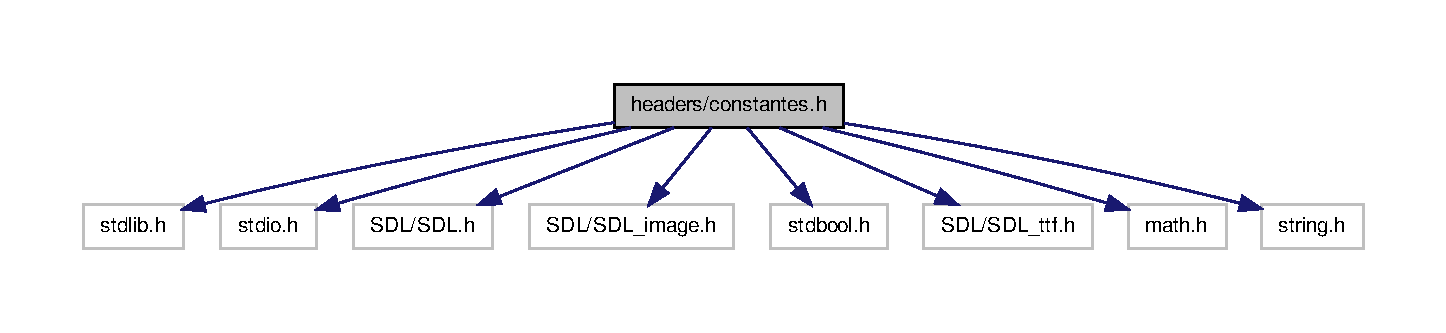
\includegraphics[width=350pt]{constantes_8h__incl}
\end{center}
\end{figure}
\-Ce graphe montre quels fichiers incluent directement ou indirectement ce fichier \-:
\nopagebreak
\begin{figure}[H]
\begin{center}
\leavevmode
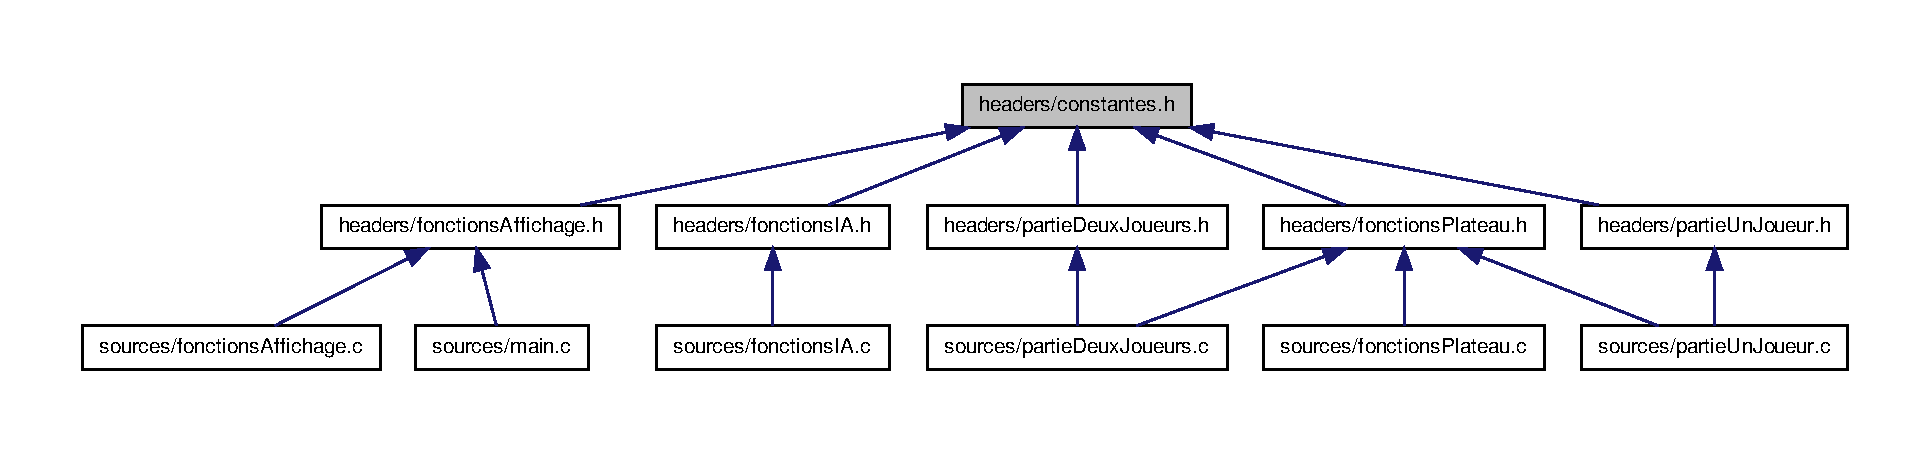
\includegraphics[width=350pt]{constantes_8h__dep__incl}
\end{center}
\end{figure}
\subsection*{\-Macros}
\begin{DoxyCompactItemize}
\item 
\#define \hyperlink{constantes_8h_a6068a247ff9ece1b0a9773c58144906c}{\-L\-A\-R\-G\-E\-U\-R\-\_\-\-F\-E\-N\-E\-T\-R\-E}~800
\item 
\#define \hyperlink{constantes_8h_afd1a1e285af564b849b17498e82e1a41}{\-H\-A\-U\-T\-E\-U\-R\-\_\-\-F\-E\-N\-E\-T\-R\-E}~500
\item 
\#define \hyperlink{constantes_8h_abff55699e9fdf03f67a0279aa5c84ebe}{\-D\-I\-M\-\_\-\-P\-L\-A\-T\-E\-A\-U}~6
\item 
\#define \hyperlink{constantes_8h_a256cf95d6901a0a5cb59dbfe010ea629}{\-T\-A\-I\-L\-L\-E\-\_\-\-E\-M\-P\-L\-A\-C\-E\-M\-E\-N\-T}~50
\item 
\#define \hyperlink{constantes_8h_a1ebe07e8d51bd8a62e93b465d5c1161c}{\-R\-A\-Y\-O\-N\-\_\-\-B\-I\-L\-L\-E}~17
\item 
\hypertarget{constantes_8h_a578685cf873cd8e2d73002c3cb9fbf7a}{\#define {\bfseries \-N\-B\-\_\-\-C\-O\-U\-P\-\_\-\-M\-A\-X}~(\hyperlink{constantes_8h_abff55699e9fdf03f67a0279aa5c84ebe}{\-D\-I\-M\-\_\-\-P\-L\-A\-T\-E\-A\-U}$\ast$\hyperlink{constantes_8h_abff55699e9fdf03f67a0279aa5c84ebe}{\-D\-I\-M\-\_\-\-P\-L\-A\-T\-E\-A\-U})}\label{constantes_8h_a578685cf873cd8e2d73002c3cb9fbf7a}

\item 
\#define \hyperlink{constantes_8h_a48f2466e604fccdb4211b8d5c7936077}{\-A\-B\-S\-\_\-\-P\-L\-A\-T\-E\-A\-U}~(\hyperlink{constantes_8h_a6068a247ff9ece1b0a9773c58144906c}{\-L\-A\-R\-G\-E\-U\-R\-\_\-\-F\-E\-N\-E\-T\-R\-E}/2 -\/ (\hyperlink{constantes_8h_abff55699e9fdf03f67a0279aa5c84ebe}{\-D\-I\-M\-\_\-\-P\-L\-A\-T\-E\-A\-U}$\ast$\hyperlink{constantes_8h_a256cf95d6901a0a5cb59dbfe010ea629}{\-T\-A\-I\-L\-L\-E\-\_\-\-E\-M\-P\-L\-A\-C\-E\-M\-E\-N\-T})/2)
\item 
\#define \hyperlink{constantes_8h_a7157aadd4e19b59cb629aea949da774b}{\-O\-R\-D\-\_\-\-P\-L\-A\-T\-E\-A\-U}~(\hyperlink{constantes_8h_afd1a1e285af564b849b17498e82e1a41}{\-H\-A\-U\-T\-E\-U\-R\-\_\-\-F\-E\-N\-E\-T\-R\-E}/2 -\/ (\hyperlink{constantes_8h_abff55699e9fdf03f67a0279aa5c84ebe}{\-D\-I\-M\-\_\-\-P\-L\-A\-T\-E\-A\-U}$\ast$\hyperlink{constantes_8h_a256cf95d6901a0a5cb59dbfe010ea629}{\-T\-A\-I\-L\-L\-E\-\_\-\-E\-M\-P\-L\-A\-C\-E\-M\-E\-N\-T})/2)
\item 
\#define \hyperlink{constantes_8h_a1aa17778f2187f12dea9306c3388cbf2}{\-B\-A\-S\-\_\-\-F\-E\-N\-E\-T\-R\-E}~(\hyperlink{constantes_8h_afd1a1e285af564b849b17498e82e1a41}{\-H\-A\-U\-T\-E\-U\-R\-\_\-\-F\-E\-N\-E\-T\-R\-E}-\/25)
\end{DoxyCompactItemize}
\subsection*{\-Définitions de type}
\begin{DoxyCompactItemize}
\item 
\hypertarget{constantes_8h_ac19c17e9f0f0eeec3f3c11b052cfeb47}{typedef int \hyperlink{constantes_8h_ac19c17e9f0f0eeec3f3c11b052cfeb47}{\-Plateau} \mbox{[}\hyperlink{constantes_8h_abff55699e9fdf03f67a0279aa5c84ebe}{\-D\-I\-M\-\_\-\-P\-L\-A\-T\-E\-A\-U}\mbox{]}\mbox{[}\hyperlink{constantes_8h_abff55699e9fdf03f67a0279aa5c84ebe}{\-D\-I\-M\-\_\-\-P\-L\-A\-T\-E\-A\-U}\mbox{]}}\label{constantes_8h_ac19c17e9f0f0eeec3f3c11b052cfeb47}

\begin{DoxyCompactList}\small\item\em \-Le \-Plateau du jeu est un tableau à deux dimensions de \-D\-I\-M\-\_\-\-P\-L\-A\-T\-E\-A\-U$\ast$\-D\-I\-M\-\_\-\-P\-L\-A\-T\-E\-A\-U cases. \end{DoxyCompactList}\end{DoxyCompactItemize}
\subsection*{Énumérations}
\begin{DoxyCompactItemize}
\item 
enum \hyperlink{constantes_8h_a50c2270bee9c93a5fee9353a453ade4d}{contenu\-Case} \{ \hyperlink{constantes_8h_a50c2270bee9c93a5fee9353a453ade4da59e3323a198f0162330111165caaf367}{\-N\-O\-I\-R}, 
\hyperlink{constantes_8h_a50c2270bee9c93a5fee9353a453ade4da35653913ced93d8199f0378ec538a0c7}{\-B\-L\-A\-N\-C}, 
\hyperlink{constantes_8h_a50c2270bee9c93a5fee9353a453ade4dad4686f4f969d0e851d9170c09a89a837}{\-V\-I\-D\-E}
 \}
\begin{DoxyCompactList}\small\item\em \-Représente le contenue d une case. \end{DoxyCompactList}\item 
enum \hyperlink{constantes_8h_a957d49625acff3240684bc203fdb2be9}{partie\-Plateau} \{ \hyperlink{constantes_8h_a957d49625acff3240684bc203fdb2be9a4dd42713302f94f70f81a7fc5ea8d471}{\-H\-A\-U\-T\-\_\-\-G\-A\-U\-C\-H\-E}, 
\hyperlink{constantes_8h_a957d49625acff3240684bc203fdb2be9ae03ba231106011b859289ef76eb6fb4c}{\-H\-A\-U\-T\-\_\-\-D\-R\-O\-I\-T\-E}, 
\hyperlink{constantes_8h_a957d49625acff3240684bc203fdb2be9a5ec7ee2eeade21efcc17a56557f9eec8}{\-B\-A\-S\-\_\-\-G\-A\-U\-C\-H\-E}, 
\hyperlink{constantes_8h_a957d49625acff3240684bc203fdb2be9a5abf263122ab0d263c9ec808386960f8}{\-B\-A\-S\-\_\-\-D\-R\-O\-I\-T\-E}
 \}
\item 
enum \hyperlink{constantes_8h_adfeae4fcbc73ce28fdbb0b2e9e0aa5dd}{gagnant} \{ \hyperlink{constantes_8h_adfeae4fcbc73ce28fdbb0b2e9e0aa5dda7a14fc427a3e7002251f769b8e99c031}{\-N\-O\-I\-R\-\_\-\-G\-A\-G\-N\-A\-N\-T}, 
\hyperlink{constantes_8h_adfeae4fcbc73ce28fdbb0b2e9e0aa5ddafa740ceaf24189b31027f49c3ff00bd7}{\-B\-L\-A\-N\-C\-\_\-\-G\-A\-G\-N\-A\-N\-T}, 
\hyperlink{constantes_8h_adfeae4fcbc73ce28fdbb0b2e9e0aa5ddafd9621762996b1efb156550dc37b2be4}{\-P\-E\-R\-S\-O\-N\-N\-E}, 
\hyperlink{constantes_8h_adfeae4fcbc73ce28fdbb0b2e9e0aa5dda5ce063289dc687d6c5ea8cddc448f583}{\-E\-G\-A\-L\-I\-T\-E}
 \}
\begin{DoxyCompactList}\small\item\em \-Représente le gagnant. \end{DoxyCompactList}\item 
enum \hyperlink{constantes_8h_aa65e3b592c27609a542733310b34f5d9}{sens} \{ \hyperlink{constantes_8h_aa65e3b592c27609a542733310b34f5d9a256d855045cd690afdadf5fd09db25cb}{\-S\-E\-N\-S\-\_\-\-H\-O\-R\-A\-I\-R\-E}, 
\hyperlink{constantes_8h_aa65e3b592c27609a542733310b34f5d9ad231635c9a6617d63f6e644ffba30370}{\-S\-E\-N\-S\-\_\-\-T\-R\-I\-G\-O\-N\-O\-M\-E\-T\-R\-I\-Q\-U\-E}
 \}
\begin{DoxyCompactList}\small\item\em \-Représente le sens de la rotation. \end{DoxyCompactList}\item 
enum \hyperlink{constantes_8h_a905479d79c2aa8410d2fc374bc75cc5b}{menu} \{ \*
\hyperlink{constantes_8h_a905479d79c2aa8410d2fc374bc75cc5ba70b100093f9f5e4ec3406859cc808132}{\-R\-I\-E\-N}, 
\hyperlink{constantes_8h_a905479d79c2aa8410d2fc374bc75cc5bab5ff09f1f071ccf03e71e867b696f7a0}{\-M\-O\-D\-E\-\_\-\-U\-N\-\_\-\-J\-O\-U\-E\-U\-R}, 
\hyperlink{constantes_8h_a905479d79c2aa8410d2fc374bc75cc5babf4d263385fdac45dc9057141dfc05f1}{\-M\-O\-D\-E\-\_\-\-D\-E\-U\-X\-\_\-\-J\-O\-U\-E\-U\-R}, 
\hyperlink{constantes_8h_a905479d79c2aa8410d2fc374bc75cc5ba34fee33b89d4454c2a79b0ee5f84b2a3}{\-R\-E\-G\-L\-E}, 
\*
\hyperlink{constantes_8h_a905479d79c2aa8410d2fc374bc75cc5ba823bd8d0ae9f7847c8e13b3d6fdb0d4b}{\-P\-R\-O\-P\-O\-S}, 
\hyperlink{constantes_8h_a905479d79c2aa8410d2fc374bc75cc5ba8e639928892ca56805cccf6606dcff63}{\-Q\-U\-I\-T\-T\-E\-R}
 \}
\begin{DoxyCompactList}\small\item\em \-Représente un item du menu. \end{DoxyCompactList}\end{DoxyCompactItemize}


\subsection{\-Description détaillée}
définitions de constantes 

\subsection{\-Documentation des macros}
\hypertarget{constantes_8h_a48f2466e604fccdb4211b8d5c7936077}{\index{constantes.\-h@{constantes.\-h}!\-A\-B\-S\-\_\-\-P\-L\-A\-T\-E\-A\-U@{\-A\-B\-S\-\_\-\-P\-L\-A\-T\-E\-A\-U}}
\index{\-A\-B\-S\-\_\-\-P\-L\-A\-T\-E\-A\-U@{\-A\-B\-S\-\_\-\-P\-L\-A\-T\-E\-A\-U}!constantes.h@{constantes.\-h}}
\subsubsection[{\-A\-B\-S\-\_\-\-P\-L\-A\-T\-E\-A\-U}]{\setlength{\rightskip}{0pt plus 5cm}\#define {\bf \-A\-B\-S\-\_\-\-P\-L\-A\-T\-E\-A\-U}~({\bf \-L\-A\-R\-G\-E\-U\-R\-\_\-\-F\-E\-N\-E\-T\-R\-E}/2 -\/ ({\bf \-D\-I\-M\-\_\-\-P\-L\-A\-T\-E\-A\-U}$\ast${\bf \-T\-A\-I\-L\-L\-E\-\_\-\-E\-M\-P\-L\-A\-C\-E\-M\-E\-N\-T})/2)}}\label{constantes_8h_a48f2466e604fccdb4211b8d5c7936077}
definition d'un nouvel abscice où l'origine est le début du plateau \hypertarget{constantes_8h_a1aa17778f2187f12dea9306c3388cbf2}{\index{constantes.\-h@{constantes.\-h}!\-B\-A\-S\-\_\-\-F\-E\-N\-E\-T\-R\-E@{\-B\-A\-S\-\_\-\-F\-E\-N\-E\-T\-R\-E}}
\index{\-B\-A\-S\-\_\-\-F\-E\-N\-E\-T\-R\-E@{\-B\-A\-S\-\_\-\-F\-E\-N\-E\-T\-R\-E}!constantes.h@{constantes.\-h}}
\subsubsection[{\-B\-A\-S\-\_\-\-F\-E\-N\-E\-T\-R\-E}]{\setlength{\rightskip}{0pt plus 5cm}\#define {\bf \-B\-A\-S\-\_\-\-F\-E\-N\-E\-T\-R\-E}~({\bf \-H\-A\-U\-T\-E\-U\-R\-\_\-\-F\-E\-N\-E\-T\-R\-E}-\/25)}}\label{constantes_8h_a1aa17778f2187f12dea9306c3388cbf2}
definition du bas de la fenètre pour le menu miniature \hypertarget{constantes_8h_abff55699e9fdf03f67a0279aa5c84ebe}{\index{constantes.\-h@{constantes.\-h}!\-D\-I\-M\-\_\-\-P\-L\-A\-T\-E\-A\-U@{\-D\-I\-M\-\_\-\-P\-L\-A\-T\-E\-A\-U}}
\index{\-D\-I\-M\-\_\-\-P\-L\-A\-T\-E\-A\-U@{\-D\-I\-M\-\_\-\-P\-L\-A\-T\-E\-A\-U}!constantes.h@{constantes.\-h}}
\subsubsection[{\-D\-I\-M\-\_\-\-P\-L\-A\-T\-E\-A\-U}]{\setlength{\rightskip}{0pt plus 5cm}\#define {\bf \-D\-I\-M\-\_\-\-P\-L\-A\-T\-E\-A\-U}~6}}\label{constantes_8h_abff55699e9fdf03f67a0279aa5c84ebe}
definition du plateau de \-D\-I\-M\-\_\-\-P\-L\-A\-T\-E\-U$\ast$\-D\-I\-M\-\_\-\-P\-L\-A\-T\-E\-A\-U emplacement \hypertarget{constantes_8h_afd1a1e285af564b849b17498e82e1a41}{\index{constantes.\-h@{constantes.\-h}!\-H\-A\-U\-T\-E\-U\-R\-\_\-\-F\-E\-N\-E\-T\-R\-E@{\-H\-A\-U\-T\-E\-U\-R\-\_\-\-F\-E\-N\-E\-T\-R\-E}}
\index{\-H\-A\-U\-T\-E\-U\-R\-\_\-\-F\-E\-N\-E\-T\-R\-E@{\-H\-A\-U\-T\-E\-U\-R\-\_\-\-F\-E\-N\-E\-T\-R\-E}!constantes.h@{constantes.\-h}}
\subsubsection[{\-H\-A\-U\-T\-E\-U\-R\-\_\-\-F\-E\-N\-E\-T\-R\-E}]{\setlength{\rightskip}{0pt plus 5cm}\#define {\bf \-H\-A\-U\-T\-E\-U\-R\-\_\-\-F\-E\-N\-E\-T\-R\-E}~500}}\label{constantes_8h_afd1a1e285af564b849b17498e82e1a41}
\-La hauteur de notre fenetre de jeu \hypertarget{constantes_8h_a6068a247ff9ece1b0a9773c58144906c}{\index{constantes.\-h@{constantes.\-h}!\-L\-A\-R\-G\-E\-U\-R\-\_\-\-F\-E\-N\-E\-T\-R\-E@{\-L\-A\-R\-G\-E\-U\-R\-\_\-\-F\-E\-N\-E\-T\-R\-E}}
\index{\-L\-A\-R\-G\-E\-U\-R\-\_\-\-F\-E\-N\-E\-T\-R\-E@{\-L\-A\-R\-G\-E\-U\-R\-\_\-\-F\-E\-N\-E\-T\-R\-E}!constantes.h@{constantes.\-h}}
\subsubsection[{\-L\-A\-R\-G\-E\-U\-R\-\_\-\-F\-E\-N\-E\-T\-R\-E}]{\setlength{\rightskip}{0pt plus 5cm}\#define {\bf \-L\-A\-R\-G\-E\-U\-R\-\_\-\-F\-E\-N\-E\-T\-R\-E}~800}}\label{constantes_8h_a6068a247ff9ece1b0a9773c58144906c}
\-La largeur de notre fenetre de jeu \hypertarget{constantes_8h_a7157aadd4e19b59cb629aea949da774b}{\index{constantes.\-h@{constantes.\-h}!\-O\-R\-D\-\_\-\-P\-L\-A\-T\-E\-A\-U@{\-O\-R\-D\-\_\-\-P\-L\-A\-T\-E\-A\-U}}
\index{\-O\-R\-D\-\_\-\-P\-L\-A\-T\-E\-A\-U@{\-O\-R\-D\-\_\-\-P\-L\-A\-T\-E\-A\-U}!constantes.h@{constantes.\-h}}
\subsubsection[{\-O\-R\-D\-\_\-\-P\-L\-A\-T\-E\-A\-U}]{\setlength{\rightskip}{0pt plus 5cm}\#define {\bf \-O\-R\-D\-\_\-\-P\-L\-A\-T\-E\-A\-U}~({\bf \-H\-A\-U\-T\-E\-U\-R\-\_\-\-F\-E\-N\-E\-T\-R\-E}/2 -\/ ({\bf \-D\-I\-M\-\_\-\-P\-L\-A\-T\-E\-A\-U}$\ast${\bf \-T\-A\-I\-L\-L\-E\-\_\-\-E\-M\-P\-L\-A\-C\-E\-M\-E\-N\-T})/2)}}\label{constantes_8h_a7157aadd4e19b59cb629aea949da774b}
definition d'un nouvel ordonnée où l'origine est le début du plateau \hypertarget{constantes_8h_a1ebe07e8d51bd8a62e93b465d5c1161c}{\index{constantes.\-h@{constantes.\-h}!\-R\-A\-Y\-O\-N\-\_\-\-B\-I\-L\-L\-E@{\-R\-A\-Y\-O\-N\-\_\-\-B\-I\-L\-L\-E}}
\index{\-R\-A\-Y\-O\-N\-\_\-\-B\-I\-L\-L\-E@{\-R\-A\-Y\-O\-N\-\_\-\-B\-I\-L\-L\-E}!constantes.h@{constantes.\-h}}
\subsubsection[{\-R\-A\-Y\-O\-N\-\_\-\-B\-I\-L\-L\-E}]{\setlength{\rightskip}{0pt plus 5cm}\#define {\bf \-R\-A\-Y\-O\-N\-\_\-\-B\-I\-L\-L\-E}~17}}\label{constantes_8h_a1ebe07e8d51bd8a62e93b465d5c1161c}
definition de la taille d'un compartiment pour une bille \hypertarget{constantes_8h_a256cf95d6901a0a5cb59dbfe010ea629}{\index{constantes.\-h@{constantes.\-h}!\-T\-A\-I\-L\-L\-E\-\_\-\-E\-M\-P\-L\-A\-C\-E\-M\-E\-N\-T@{\-T\-A\-I\-L\-L\-E\-\_\-\-E\-M\-P\-L\-A\-C\-E\-M\-E\-N\-T}}
\index{\-T\-A\-I\-L\-L\-E\-\_\-\-E\-M\-P\-L\-A\-C\-E\-M\-E\-N\-T@{\-T\-A\-I\-L\-L\-E\-\_\-\-E\-M\-P\-L\-A\-C\-E\-M\-E\-N\-T}!constantes.h@{constantes.\-h}}
\subsubsection[{\-T\-A\-I\-L\-L\-E\-\_\-\-E\-M\-P\-L\-A\-C\-E\-M\-E\-N\-T}]{\setlength{\rightskip}{0pt plus 5cm}\#define {\bf \-T\-A\-I\-L\-L\-E\-\_\-\-E\-M\-P\-L\-A\-C\-E\-M\-E\-N\-T}~50}}\label{constantes_8h_a256cf95d6901a0a5cb59dbfe010ea629}
definition de la taille d'un emplacement pour une bille 

\subsection{\-Documentation du type de l'énumération}
\hypertarget{constantes_8h_a50c2270bee9c93a5fee9353a453ade4d}{\index{constantes.\-h@{constantes.\-h}!contenu\-Case@{contenu\-Case}}
\index{contenu\-Case@{contenu\-Case}!constantes.h@{constantes.\-h}}
\subsubsection[{contenu\-Case}]{\setlength{\rightskip}{0pt plus 5cm}enum {\bf contenu\-Case}}}\label{constantes_8h_a50c2270bee9c93a5fee9353a453ade4d}


\-Représente le contenue d une case. 

\begin{Desc}
\item[\-Valeurs énumérées\-: ]\par
\begin{description}
\index{\-N\-O\-I\-R@{\-N\-O\-I\-R}!constantes.\-h@{constantes.\-h}}\index{constantes.\-h@{constantes.\-h}!\-N\-O\-I\-R@{\-N\-O\-I\-R}}\item[{\em 
\hypertarget{constantes_8h_a50c2270bee9c93a5fee9353a453ade4da59e3323a198f0162330111165caaf367}{\-N\-O\-I\-R}\label{constantes_8h_a50c2270bee9c93a5fee9353a453ade4da59e3323a198f0162330111165caaf367}
}]case avec une bille noire \index{\-B\-L\-A\-N\-C@{\-B\-L\-A\-N\-C}!constantes.\-h@{constantes.\-h}}\index{constantes.\-h@{constantes.\-h}!\-B\-L\-A\-N\-C@{\-B\-L\-A\-N\-C}}\item[{\em 
\hypertarget{constantes_8h_a50c2270bee9c93a5fee9353a453ade4da35653913ced93d8199f0378ec538a0c7}{\-B\-L\-A\-N\-C}\label{constantes_8h_a50c2270bee9c93a5fee9353a453ade4da35653913ced93d8199f0378ec538a0c7}
}]case avec une bille blanche \index{\-V\-I\-D\-E@{\-V\-I\-D\-E}!constantes.\-h@{constantes.\-h}}\index{constantes.\-h@{constantes.\-h}!\-V\-I\-D\-E@{\-V\-I\-D\-E}}\item[{\em 
\hypertarget{constantes_8h_a50c2270bee9c93a5fee9353a453ade4dad4686f4f969d0e851d9170c09a89a837}{\-V\-I\-D\-E}\label{constantes_8h_a50c2270bee9c93a5fee9353a453ade4dad4686f4f969d0e851d9170c09a89a837}
}]case vide \end{description}
\end{Desc}

\hypertarget{constantes_8h_adfeae4fcbc73ce28fdbb0b2e9e0aa5dd}{\index{constantes.\-h@{constantes.\-h}!gagnant@{gagnant}}
\index{gagnant@{gagnant}!constantes.h@{constantes.\-h}}
\subsubsection[{gagnant}]{\setlength{\rightskip}{0pt plus 5cm}enum {\bf gagnant}}}\label{constantes_8h_adfeae4fcbc73ce28fdbb0b2e9e0aa5dd}


\-Représente le gagnant. 

\begin{Desc}
\item[\-Valeurs énumérées\-: ]\par
\begin{description}
\index{\-N\-O\-I\-R\-\_\-\-G\-A\-G\-N\-A\-N\-T@{\-N\-O\-I\-R\-\_\-\-G\-A\-G\-N\-A\-N\-T}!constantes.\-h@{constantes.\-h}}\index{constantes.\-h@{constantes.\-h}!\-N\-O\-I\-R\-\_\-\-G\-A\-G\-N\-A\-N\-T@{\-N\-O\-I\-R\-\_\-\-G\-A\-G\-N\-A\-N\-T}}\item[{\em 
\hypertarget{constantes_8h_adfeae4fcbc73ce28fdbb0b2e9e0aa5dda7a14fc427a3e7002251f769b8e99c031}{\-N\-O\-I\-R\-\_\-\-G\-A\-G\-N\-A\-N\-T}\label{constantes_8h_adfeae4fcbc73ce28fdbb0b2e9e0aa5dda7a14fc427a3e7002251f769b8e99c031}
}]\-Represente le cas où le joueur noir gagne \index{\-B\-L\-A\-N\-C\-\_\-\-G\-A\-G\-N\-A\-N\-T@{\-B\-L\-A\-N\-C\-\_\-\-G\-A\-G\-N\-A\-N\-T}!constantes.\-h@{constantes.\-h}}\index{constantes.\-h@{constantes.\-h}!\-B\-L\-A\-N\-C\-\_\-\-G\-A\-G\-N\-A\-N\-T@{\-B\-L\-A\-N\-C\-\_\-\-G\-A\-G\-N\-A\-N\-T}}\item[{\em 
\hypertarget{constantes_8h_adfeae4fcbc73ce28fdbb0b2e9e0aa5ddafa740ceaf24189b31027f49c3ff00bd7}{\-B\-L\-A\-N\-C\-\_\-\-G\-A\-G\-N\-A\-N\-T}\label{constantes_8h_adfeae4fcbc73ce28fdbb0b2e9e0aa5ddafa740ceaf24189b31027f49c3ff00bd7}
}]\-Represente le cas où le joueur blanc gagne \index{\-P\-E\-R\-S\-O\-N\-N\-E@{\-P\-E\-R\-S\-O\-N\-N\-E}!constantes.\-h@{constantes.\-h}}\index{constantes.\-h@{constantes.\-h}!\-P\-E\-R\-S\-O\-N\-N\-E@{\-P\-E\-R\-S\-O\-N\-N\-E}}\item[{\em 
\hypertarget{constantes_8h_adfeae4fcbc73ce28fdbb0b2e9e0aa5ddafd9621762996b1efb156550dc37b2be4}{\-P\-E\-R\-S\-O\-N\-N\-E}\label{constantes_8h_adfeae4fcbc73ce28fdbb0b2e9e0aa5ddafd9621762996b1efb156550dc37b2be4}
}]\-Represente le cas où personne gagne \index{\-E\-G\-A\-L\-I\-T\-E@{\-E\-G\-A\-L\-I\-T\-E}!constantes.\-h@{constantes.\-h}}\index{constantes.\-h@{constantes.\-h}!\-E\-G\-A\-L\-I\-T\-E@{\-E\-G\-A\-L\-I\-T\-E}}\item[{\em 
\hypertarget{constantes_8h_adfeae4fcbc73ce28fdbb0b2e9e0aa5dda5ce063289dc687d6c5ea8cddc448f583}{\-E\-G\-A\-L\-I\-T\-E}\label{constantes_8h_adfeae4fcbc73ce28fdbb0b2e9e0aa5dda5ce063289dc687d6c5ea8cddc448f583}
}]\-Represente l'égalité \end{description}
\end{Desc}

\hypertarget{constantes_8h_a905479d79c2aa8410d2fc374bc75cc5b}{\index{constantes.\-h@{constantes.\-h}!menu@{menu}}
\index{menu@{menu}!constantes.h@{constantes.\-h}}
\subsubsection[{menu}]{\setlength{\rightskip}{0pt plus 5cm}enum {\bf menu}}}\label{constantes_8h_a905479d79c2aa8410d2fc374bc75cc5b}


\-Représente un item du menu. 

\begin{Desc}
\item[\-Valeurs énumérées\-: ]\par
\begin{description}
\index{\-R\-I\-E\-N@{\-R\-I\-E\-N}!constantes.\-h@{constantes.\-h}}\index{constantes.\-h@{constantes.\-h}!\-R\-I\-E\-N@{\-R\-I\-E\-N}}\item[{\em 
\hypertarget{constantes_8h_a905479d79c2aa8410d2fc374bc75cc5ba70b100093f9f5e4ec3406859cc808132}{\-R\-I\-E\-N}\label{constantes_8h_a905479d79c2aa8410d2fc374bc75cc5ba70b100093f9f5e4ec3406859cc808132}
}]\-Represente le cas où on reste dans le menu \index{\-M\-O\-D\-E\-\_\-\-U\-N\-\_\-\-J\-O\-U\-E\-U\-R@{\-M\-O\-D\-E\-\_\-\-U\-N\-\_\-\-J\-O\-U\-E\-U\-R}!constantes.\-h@{constantes.\-h}}\index{constantes.\-h@{constantes.\-h}!\-M\-O\-D\-E\-\_\-\-U\-N\-\_\-\-J\-O\-U\-E\-U\-R@{\-M\-O\-D\-E\-\_\-\-U\-N\-\_\-\-J\-O\-U\-E\-U\-R}}\item[{\em 
\hypertarget{constantes_8h_a905479d79c2aa8410d2fc374bc75cc5bab5ff09f1f071ccf03e71e867b696f7a0}{\-M\-O\-D\-E\-\_\-\-U\-N\-\_\-\-J\-O\-U\-E\-U\-R}\label{constantes_8h_a905479d79c2aa8410d2fc374bc75cc5bab5ff09f1f071ccf03e71e867b696f7a0}
}]\-Represente le cas où on lance une partie contre l'ia \index{\-M\-O\-D\-E\-\_\-\-D\-E\-U\-X\-\_\-\-J\-O\-U\-E\-U\-R@{\-M\-O\-D\-E\-\_\-\-D\-E\-U\-X\-\_\-\-J\-O\-U\-E\-U\-R}!constantes.\-h@{constantes.\-h}}\index{constantes.\-h@{constantes.\-h}!\-M\-O\-D\-E\-\_\-\-D\-E\-U\-X\-\_\-\-J\-O\-U\-E\-U\-R@{\-M\-O\-D\-E\-\_\-\-D\-E\-U\-X\-\_\-\-J\-O\-U\-E\-U\-R}}\item[{\em 
\hypertarget{constantes_8h_a905479d79c2aa8410d2fc374bc75cc5babf4d263385fdac45dc9057141dfc05f1}{\-M\-O\-D\-E\-\_\-\-D\-E\-U\-X\-\_\-\-J\-O\-U\-E\-U\-R}\label{constantes_8h_a905479d79c2aa8410d2fc374bc75cc5babf4d263385fdac45dc9057141dfc05f1}
}]\-Represente le cas où on lance une partie contre un autre joueur \index{\-R\-E\-G\-L\-E@{\-R\-E\-G\-L\-E}!constantes.\-h@{constantes.\-h}}\index{constantes.\-h@{constantes.\-h}!\-R\-E\-G\-L\-E@{\-R\-E\-G\-L\-E}}\item[{\em 
\hypertarget{constantes_8h_a905479d79c2aa8410d2fc374bc75cc5ba34fee33b89d4454c2a79b0ee5f84b2a3}{\-R\-E\-G\-L\-E}\label{constantes_8h_a905479d79c2aa8410d2fc374bc75cc5ba34fee33b89d4454c2a79b0ee5f84b2a3}
}]\-Represente le cas où on choisit de regarder les règles du jeu \index{\-P\-R\-O\-P\-O\-S@{\-P\-R\-O\-P\-O\-S}!constantes.\-h@{constantes.\-h}}\index{constantes.\-h@{constantes.\-h}!\-P\-R\-O\-P\-O\-S@{\-P\-R\-O\-P\-O\-S}}\item[{\em 
\hypertarget{constantes_8h_a905479d79c2aa8410d2fc374bc75cc5ba823bd8d0ae9f7847c8e13b3d6fdb0d4b}{\-P\-R\-O\-P\-O\-S}\label{constantes_8h_a905479d79c2aa8410d2fc374bc75cc5ba823bd8d0ae9f7847c8e13b3d6fdb0d4b}
}]\-Represente le cas ou on choisi de regarder les information sur le jeu \index{\-Q\-U\-I\-T\-T\-E\-R@{\-Q\-U\-I\-T\-T\-E\-R}!constantes.\-h@{constantes.\-h}}\index{constantes.\-h@{constantes.\-h}!\-Q\-U\-I\-T\-T\-E\-R@{\-Q\-U\-I\-T\-T\-E\-R}}\item[{\em 
\hypertarget{constantes_8h_a905479d79c2aa8410d2fc374bc75cc5ba8e639928892ca56805cccf6606dcff63}{\-Q\-U\-I\-T\-T\-E\-R}\label{constantes_8h_a905479d79c2aa8410d2fc374bc75cc5ba8e639928892ca56805cccf6606dcff63}
}]\-Represente le cas où on choisit de quitter le jeu \end{description}
\end{Desc}

\hypertarget{constantes_8h_a957d49625acff3240684bc203fdb2be9}{\index{constantes.\-h@{constantes.\-h}!partie\-Plateau@{partie\-Plateau}}
\index{partie\-Plateau@{partie\-Plateau}!constantes.h@{constantes.\-h}}
\subsubsection[{partie\-Plateau}]{\setlength{\rightskip}{0pt plus 5cm}enum {\bf partie\-Plateau}}}\label{constantes_8h_a957d49625acff3240684bc203fdb2be9}
\begin{Desc}
\item[\-Valeurs énumérées\-: ]\par
\begin{description}
\index{\-H\-A\-U\-T\-\_\-\-G\-A\-U\-C\-H\-E@{\-H\-A\-U\-T\-\_\-\-G\-A\-U\-C\-H\-E}!constantes.\-h@{constantes.\-h}}\index{constantes.\-h@{constantes.\-h}!\-H\-A\-U\-T\-\_\-\-G\-A\-U\-C\-H\-E@{\-H\-A\-U\-T\-\_\-\-G\-A\-U\-C\-H\-E}}\item[{\em 
\hypertarget{constantes_8h_a957d49625acff3240684bc203fdb2be9a4dd42713302f94f70f81a7fc5ea8d471}{\-H\-A\-U\-T\-\_\-\-G\-A\-U\-C\-H\-E}\label{constantes_8h_a957d49625acff3240684bc203fdb2be9a4dd42713302f94f70f81a7fc5ea8d471}
}]\-Partie située en haut à gauche du plateau \index{\-H\-A\-U\-T\-\_\-\-D\-R\-O\-I\-T\-E@{\-H\-A\-U\-T\-\_\-\-D\-R\-O\-I\-T\-E}!constantes.\-h@{constantes.\-h}}\index{constantes.\-h@{constantes.\-h}!\-H\-A\-U\-T\-\_\-\-D\-R\-O\-I\-T\-E@{\-H\-A\-U\-T\-\_\-\-D\-R\-O\-I\-T\-E}}\item[{\em 
\hypertarget{constantes_8h_a957d49625acff3240684bc203fdb2be9ae03ba231106011b859289ef76eb6fb4c}{\-H\-A\-U\-T\-\_\-\-D\-R\-O\-I\-T\-E}\label{constantes_8h_a957d49625acff3240684bc203fdb2be9ae03ba231106011b859289ef76eb6fb4c}
}]\-Partie située en haut à droite du plateau \index{\-B\-A\-S\-\_\-\-G\-A\-U\-C\-H\-E@{\-B\-A\-S\-\_\-\-G\-A\-U\-C\-H\-E}!constantes.\-h@{constantes.\-h}}\index{constantes.\-h@{constantes.\-h}!\-B\-A\-S\-\_\-\-G\-A\-U\-C\-H\-E@{\-B\-A\-S\-\_\-\-G\-A\-U\-C\-H\-E}}\item[{\em 
\hypertarget{constantes_8h_a957d49625acff3240684bc203fdb2be9a5ec7ee2eeade21efcc17a56557f9eec8}{\-B\-A\-S\-\_\-\-G\-A\-U\-C\-H\-E}\label{constantes_8h_a957d49625acff3240684bc203fdb2be9a5ec7ee2eeade21efcc17a56557f9eec8}
}]\-Partie située en bas à gauche du plateau \index{\-B\-A\-S\-\_\-\-D\-R\-O\-I\-T\-E@{\-B\-A\-S\-\_\-\-D\-R\-O\-I\-T\-E}!constantes.\-h@{constantes.\-h}}\index{constantes.\-h@{constantes.\-h}!\-B\-A\-S\-\_\-\-D\-R\-O\-I\-T\-E@{\-B\-A\-S\-\_\-\-D\-R\-O\-I\-T\-E}}\item[{\em 
\hypertarget{constantes_8h_a957d49625acff3240684bc203fdb2be9a5abf263122ab0d263c9ec808386960f8}{\-B\-A\-S\-\_\-\-D\-R\-O\-I\-T\-E}\label{constantes_8h_a957d49625acff3240684bc203fdb2be9a5abf263122ab0d263c9ec808386960f8}
}]\-Partie située en bas à droite du plateau \end{description}
\end{Desc}

\hypertarget{constantes_8h_aa65e3b592c27609a542733310b34f5d9}{\index{constantes.\-h@{constantes.\-h}!sens@{sens}}
\index{sens@{sens}!constantes.h@{constantes.\-h}}
\subsubsection[{sens}]{\setlength{\rightskip}{0pt plus 5cm}enum {\bf sens}}}\label{constantes_8h_aa65e3b592c27609a542733310b34f5d9}


\-Représente le sens de la rotation. 

\begin{Desc}
\item[\-Valeurs énumérées\-: ]\par
\begin{description}
\index{\-S\-E\-N\-S\-\_\-\-H\-O\-R\-A\-I\-R\-E@{\-S\-E\-N\-S\-\_\-\-H\-O\-R\-A\-I\-R\-E}!constantes.\-h@{constantes.\-h}}\index{constantes.\-h@{constantes.\-h}!\-S\-E\-N\-S\-\_\-\-H\-O\-R\-A\-I\-R\-E@{\-S\-E\-N\-S\-\_\-\-H\-O\-R\-A\-I\-R\-E}}\item[{\em 
\hypertarget{constantes_8h_aa65e3b592c27609a542733310b34f5d9a256d855045cd690afdadf5fd09db25cb}{\-S\-E\-N\-S\-\_\-\-H\-O\-R\-A\-I\-R\-E}\label{constantes_8h_aa65e3b592c27609a542733310b34f5d9a256d855045cd690afdadf5fd09db25cb}
}]\-Represente le cas où on tourne un plateau dans le sens horaire \index{\-S\-E\-N\-S\-\_\-\-T\-R\-I\-G\-O\-N\-O\-M\-E\-T\-R\-I\-Q\-U\-E@{\-S\-E\-N\-S\-\_\-\-T\-R\-I\-G\-O\-N\-O\-M\-E\-T\-R\-I\-Q\-U\-E}!constantes.\-h@{constantes.\-h}}\index{constantes.\-h@{constantes.\-h}!\-S\-E\-N\-S\-\_\-\-T\-R\-I\-G\-O\-N\-O\-M\-E\-T\-R\-I\-Q\-U\-E@{\-S\-E\-N\-S\-\_\-\-T\-R\-I\-G\-O\-N\-O\-M\-E\-T\-R\-I\-Q\-U\-E}}\item[{\em 
\hypertarget{constantes_8h_aa65e3b592c27609a542733310b34f5d9ad231635c9a6617d63f6e644ffba30370}{\-S\-E\-N\-S\-\_\-\-T\-R\-I\-G\-O\-N\-O\-M\-E\-T\-R\-I\-Q\-U\-E}\label{constantes_8h_aa65e3b592c27609a542733310b34f5d9ad231635c9a6617d63f6e644ffba30370}
}]\-Represente le cas où on tourne un plateau dans le sens trigonometrique \end{description}
\end{Desc}


\hypertarget{fonctions_affichage_8h}{\section{\-Référence du fichier headers/fonctions\-Affichage.h}
\label{fonctions_affichage_8h}\index{headers/fonctions\-Affichage.\-h@{headers/fonctions\-Affichage.\-h}}
}


définitions des prototypes des fonctions relatives à l'affichage et aux traitement des menus  


{\ttfamily \#include \char`\"{}constantes.\-h\char`\"{}}\*
\-Graphe des dépendances par inclusion de fonctions\-Affichage.\-h\-:
\nopagebreak
\begin{figure}[H]
\begin{center}
\leavevmode
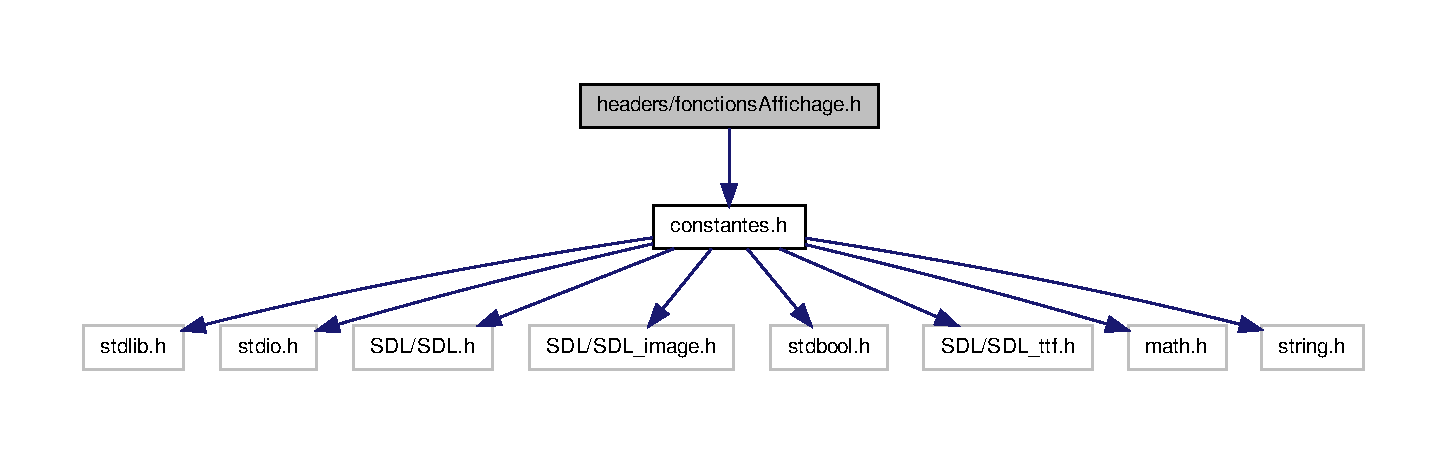
\includegraphics[width=350pt]{fonctions_affichage_8h__incl}
\end{center}
\end{figure}
\-Ce graphe montre quels fichiers incluent directement ou indirectement ce fichier \-:
\nopagebreak
\begin{figure}[H]
\begin{center}
\leavevmode
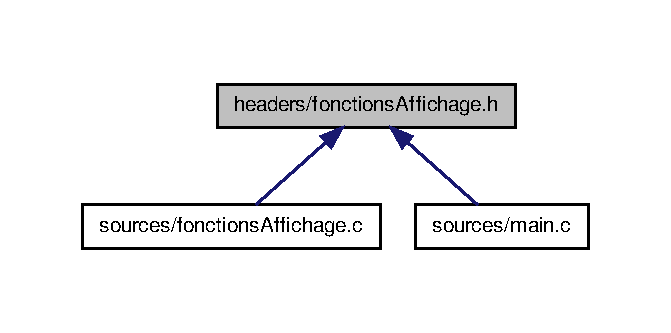
\includegraphics[width=322pt]{fonctions_affichage_8h__dep__incl}
\end{center}
\end{figure}
\subsection*{\-Fonctions}
\begin{DoxyCompactItemize}
\item 
short \hyperlink{fonctions_affichage_8h_aefaab0a4a9e4ccb284e6ce210fb6973b}{choix\-Menu} (int abs\-Clic, int ord\-Clic, \-S\-D\-L\-\_\-\-Rect pos\-Tab\-Choix\-Menu\mbox{[}$\,$\mbox{]})
\begin{DoxyCompactList}\small\item\em détermine si le joueur clique sur un des choix du menu \end{DoxyCompactList}\item 
short \hyperlink{fonctions_affichage_8h_ad5c598ce2c6742ec4c3e771488987abe}{affiche\-Regles} (\-S\-D\-L\-\_\-\-Surface $\ast$ecran)
\begin{DoxyCompactList}\small\item\em \-Affiche les rêgles du jeu. \end{DoxyCompactList}\item 
short \hyperlink{fonctions_affichage_8h_a830a6d65d1a989f174c3bcde5ae69151}{affiche\-Propos} (\-S\-D\-L\-\_\-\-Surface $\ast$ecran)
\begin{DoxyCompactList}\small\item\em \-Affiche les information sur le jeu. \end{DoxyCompactList}\item 
void \hyperlink{fonctions_affichage_8h_a6de5a4b9281294c56a4bd7254cdb481d}{affiche\-Fin} (int nom\-\_\-gagnant, int nombre\-\_\-coups, \-T\-T\-F\-\_\-\-Font $\ast$police, \-S\-D\-L\-\_\-\-Surface $\ast$texte, \-S\-D\-L\-\_\-\-Color couleur, \-S\-D\-L\-\_\-\-Surface $\ast$ecran)
\begin{DoxyCompactList}\small\item\em affiche quand une partie est terminée le nom du gagnant et le nombre de coup joué par celui ci \end{DoxyCompactList}\item 
void \hyperlink{fonctions_affichage_8h_a805c8a6f72037e8a2d3649e1ff874fa0}{affiche\-Menu\-Miniature} (\-S\-D\-L\-\_\-\-Surface $\ast$ecran, \-S\-D\-L\-\_\-\-Surface $\ast$tab\-Menu\-Miniature\mbox{[}$\,$\mbox{]}, \-S\-D\-L\-\_\-\-Rect pos\-Tab\-Menu\-Miniature\mbox{[}$\,$\mbox{]})
\begin{DoxyCompactList}\small\item\em affiche le menu miniature situé en bas de la fenêtre \end{DoxyCompactList}\item 
short \hyperlink{fonctions_affichage_8h_a48262da5b852d7d777c20285f2f0b99a}{traite\-Menu\-Miniature} (int abs\-Clic, int ord\-Clic, \-S\-D\-L\-\_\-\-Surface $\ast$ecran, int partie)
\begin{DoxyCompactList}\small\item\em détermine si le joueur clique sur un des item du menu miniature \end{DoxyCompactList}\item 
void \hyperlink{fonctions_affichage_8h_aa0b97452ac0e386637b196b6b8105c7d}{init\-Menu\-Miniature} (int partie, \-S\-D\-L\-\_\-\-Surface $\ast$tab\-Menu\-Miniature\mbox{[}$\,$\mbox{]}, \-T\-T\-F\-\_\-\-Font $\ast$police, \-S\-D\-L\-\_\-\-Color couleur)
\begin{DoxyCompactList}\small\item\em initialise le menu miniature selon la partie joué \end{DoxyCompactList}\item 
void \hyperlink{fonctions_affichage_8h_a6cede375026585c570c284965c06f83a}{affiche\-Joueur} (\-S\-D\-L\-\_\-\-Surface $\ast$ecran, int nb\-\_\-coups, \-T\-T\-F\-\_\-\-Font $\ast$police, \-S\-D\-L\-\_\-\-Color couleur)
\begin{DoxyCompactList}\small\item\em fonction affichant le joueur qui est en train de jouer \end{DoxyCompactList}\end{DoxyCompactItemize}


\subsection{\-Description détaillée}
définitions des prototypes des fonctions relatives à l'affichage et aux traitement des menus 

\subsection{\-Documentation des fonctions}
\hypertarget{fonctions_affichage_8h_a6de5a4b9281294c56a4bd7254cdb481d}{\index{fonctions\-Affichage.\-h@{fonctions\-Affichage.\-h}!affiche\-Fin@{affiche\-Fin}}
\index{affiche\-Fin@{affiche\-Fin}!fonctionsAffichage.h@{fonctions\-Affichage.\-h}}
\subsubsection[{affiche\-Fin}]{\setlength{\rightskip}{0pt plus 5cm}void {\bf affiche\-Fin} (
\begin{DoxyParamCaption}
\item[{int}]{nom\-\_\-gagnant, }
\item[{int}]{nombre\-\_\-coups, }
\item[{\-T\-T\-F\-\_\-\-Font $\ast$}]{police, }
\item[{\-S\-D\-L\-\_\-\-Surface $\ast$}]{texte, }
\item[{\-S\-D\-L\-\_\-\-Color}]{couleur, }
\item[{\-S\-D\-L\-\_\-\-Surface $\ast$}]{ecran}
\end{DoxyParamCaption}
)}}\label{fonctions_affichage_8h_a6de5a4b9281294c56a4bd7254cdb481d}


affiche quand une partie est terminée le nom du gagnant et le nombre de coup joué par celui ci 


\begin{DoxyParams}{\-Paramètres}
{\em nom\-\_\-gagnant} & le nom du gagnant conforme à l'énumération gagnant \\
\hline
{\em nombre\-\_\-coups} & le nombre de coups joué par un joueur \\
\hline
{\em police} & la police qui sert à écrire les informations \\
\hline
{\em texte} & la \-S\-D\-L\-\_\-\-Surface sur laquelle on affiche les informations \\
\hline
{\em couleur} & la couleur de la police \\
\hline
{\em ecran} & la surface \-S\-D\-L où afficher la fin \\
\hline
\end{DoxyParams}


\-Voici le graphe des appelants de cette fonction \-:
\nopagebreak
\begin{figure}[H]
\begin{center}
\leavevmode
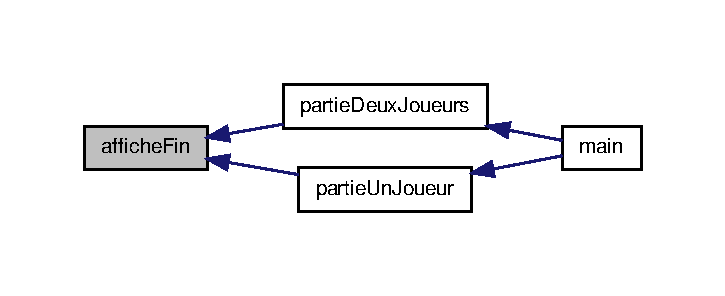
\includegraphics[width=348pt]{fonctions_affichage_8h_a6de5a4b9281294c56a4bd7254cdb481d_icgraph}
\end{center}
\end{figure}


\hypertarget{fonctions_affichage_8h_a6cede375026585c570c284965c06f83a}{\index{fonctions\-Affichage.\-h@{fonctions\-Affichage.\-h}!affiche\-Joueur@{affiche\-Joueur}}
\index{affiche\-Joueur@{affiche\-Joueur}!fonctionsAffichage.h@{fonctions\-Affichage.\-h}}
\subsubsection[{affiche\-Joueur}]{\setlength{\rightskip}{0pt plus 5cm}void {\bf affiche\-Joueur} (
\begin{DoxyParamCaption}
\item[{\-S\-D\-L\-\_\-\-Surface $\ast$}]{ecran, }
\item[{int}]{nb\-\_\-coups, }
\item[{\-T\-T\-F\-\_\-\-Font $\ast$}]{police, }
\item[{\-S\-D\-L\-\_\-\-Color}]{couleur}
\end{DoxyParamCaption}
)}}\label{fonctions_affichage_8h_a6cede375026585c570c284965c06f83a}


fonction affichant le joueur qui est en train de jouer 


\begin{DoxyParams}{\-Paramètres}
{\em ecran} & la surface \-S\-D\-L où afficher le joueur \\
\hline
{\em nb\-\_\-coups} & nombre qui nous sert a determiner le joueur courant selon le nombre de coups joué \\
\hline
{\em police} & la police utilisé \\
\hline
{\em couleur} & la couleur de la police \\
\hline
\end{DoxyParams}


\-Voici le graphe des appelants de cette fonction \-:
\nopagebreak
\begin{figure}[H]
\begin{center}
\leavevmode
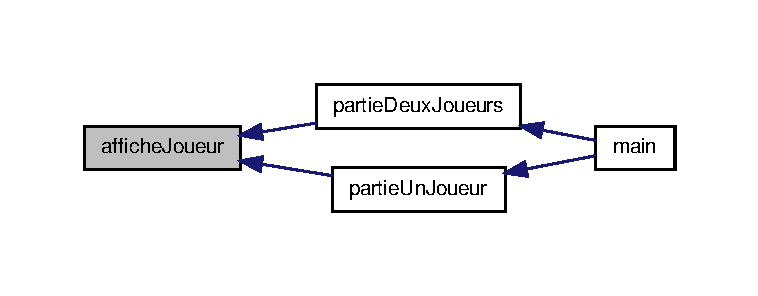
\includegraphics[width=350pt]{fonctions_affichage_8h_a6cede375026585c570c284965c06f83a_icgraph}
\end{center}
\end{figure}


\hypertarget{fonctions_affichage_8h_a805c8a6f72037e8a2d3649e1ff874fa0}{\index{fonctions\-Affichage.\-h@{fonctions\-Affichage.\-h}!affiche\-Menu\-Miniature@{affiche\-Menu\-Miniature}}
\index{affiche\-Menu\-Miniature@{affiche\-Menu\-Miniature}!fonctionsAffichage.h@{fonctions\-Affichage.\-h}}
\subsubsection[{affiche\-Menu\-Miniature}]{\setlength{\rightskip}{0pt plus 5cm}void {\bf affiche\-Menu\-Miniature} (
\begin{DoxyParamCaption}
\item[{\-S\-D\-L\-\_\-\-Surface $\ast$}]{ecran, }
\item[{\-S\-D\-L\-\_\-\-Surface $\ast$}]{tab\-Menu\-Miniature\mbox{[}$\,$\mbox{]}, }
\item[{\-S\-D\-L\-\_\-\-Rect}]{pos\-Tab\-Menu\-Miniature\mbox{[}$\,$\mbox{]}}
\end{DoxyParamCaption}
)}}\label{fonctions_affichage_8h_a805c8a6f72037e8a2d3649e1ff874fa0}


affiche le menu miniature situé en bas de la fenêtre 


\begin{DoxyParams}{\-Paramètres}
{\em ecran} & la surface \-S\-D\-L où afficher le menu miniature \\
\hline
{\em tab\-Menu\-Miniature\mbox{[}$\,$\mbox{]}} & tableau contenant les élément du menu miniature \\
\hline
{\em postab\-Menu\-Miniature\mbox{[}$\,$\mbox{]}} & tableau contenant la position des élément du menu miniature \\
\hline
\end{DoxyParams}


\-Voici le graphe des appelants de cette fonction \-:
\nopagebreak
\begin{figure}[H]
\begin{center}
\leavevmode
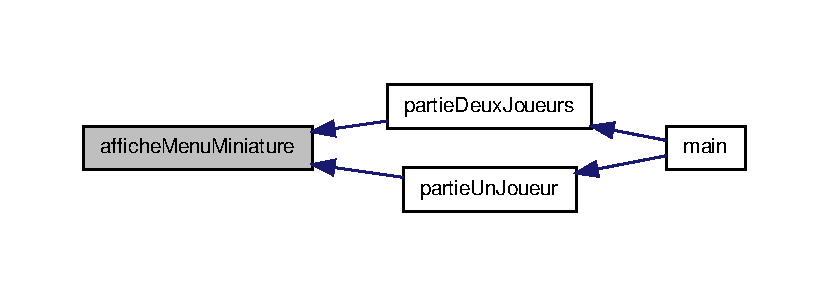
\includegraphics[width=350pt]{fonctions_affichage_8h_a805c8a6f72037e8a2d3649e1ff874fa0_icgraph}
\end{center}
\end{figure}


\hypertarget{fonctions_affichage_8h_a830a6d65d1a989f174c3bcde5ae69151}{\index{fonctions\-Affichage.\-h@{fonctions\-Affichage.\-h}!affiche\-Propos@{affiche\-Propos}}
\index{affiche\-Propos@{affiche\-Propos}!fonctionsAffichage.h@{fonctions\-Affichage.\-h}}
\subsubsection[{affiche\-Propos}]{\setlength{\rightskip}{0pt plus 5cm}short {\bf affiche\-Propos} (
\begin{DoxyParamCaption}
\item[{\-S\-D\-L\-\_\-\-Surface $\ast$}]{ecran}
\end{DoxyParamCaption}
)}}\label{fonctions_affichage_8h_a830a6d65d1a989f174c3bcde5ae69151}


\-Affiche les information sur le jeu. 


\begin{DoxyParams}{\-Paramètres}
{\em ecran} & la surface \-S\-D\-L où afficher les informations\\
\hline
\end{DoxyParams}
\begin{DoxyReturn}{\-Renvoie}
retourne \-E\-X\-I\-T\-\_\-\-S\-U\-C\-C\-E\-S\-S pour verifier si la fonction c'est exécuté normalement 
\end{DoxyReturn}


\-Voici le graphe d'appel pour cette fonction \-:
\nopagebreak
\begin{figure}[H]
\begin{center}
\leavevmode
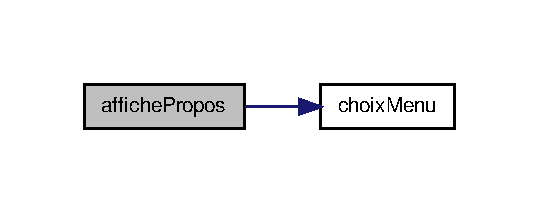
\includegraphics[width=258pt]{fonctions_affichage_8h_a830a6d65d1a989f174c3bcde5ae69151_cgraph}
\end{center}
\end{figure}




\-Voici le graphe des appelants de cette fonction \-:
\nopagebreak
\begin{figure}[H]
\begin{center}
\leavevmode
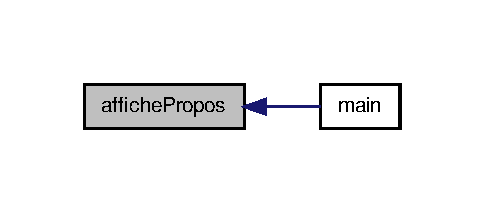
\includegraphics[width=232pt]{fonctions_affichage_8h_a830a6d65d1a989f174c3bcde5ae69151_icgraph}
\end{center}
\end{figure}


\hypertarget{fonctions_affichage_8h_ad5c598ce2c6742ec4c3e771488987abe}{\index{fonctions\-Affichage.\-h@{fonctions\-Affichage.\-h}!affiche\-Regles@{affiche\-Regles}}
\index{affiche\-Regles@{affiche\-Regles}!fonctionsAffichage.h@{fonctions\-Affichage.\-h}}
\subsubsection[{affiche\-Regles}]{\setlength{\rightskip}{0pt plus 5cm}short {\bf affiche\-Regles} (
\begin{DoxyParamCaption}
\item[{\-S\-D\-L\-\_\-\-Surface $\ast$}]{ecran}
\end{DoxyParamCaption}
)}}\label{fonctions_affichage_8h_ad5c598ce2c6742ec4c3e771488987abe}


\-Affiche les rêgles du jeu. 


\begin{DoxyParams}{\-Paramètres}
{\em ecran} & la surface \-S\-D\-L où afficher les règles\\
\hline
\end{DoxyParams}
\begin{DoxyReturn}{\-Renvoie}
retourne \-E\-X\-I\-T\-\_\-\-S\-U\-C\-C\-E\-S\-S pour verifier si la fonction c'est exécuté normalement 
\end{DoxyReturn}


\-Voici le graphe d'appel pour cette fonction \-:
\nopagebreak
\begin{figure}[H]
\begin{center}
\leavevmode
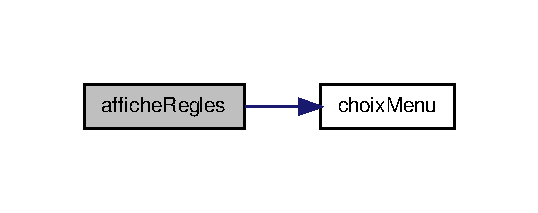
\includegraphics[width=258pt]{fonctions_affichage_8h_ad5c598ce2c6742ec4c3e771488987abe_cgraph}
\end{center}
\end{figure}




\-Voici le graphe des appelants de cette fonction \-:
\nopagebreak
\begin{figure}[H]
\begin{center}
\leavevmode
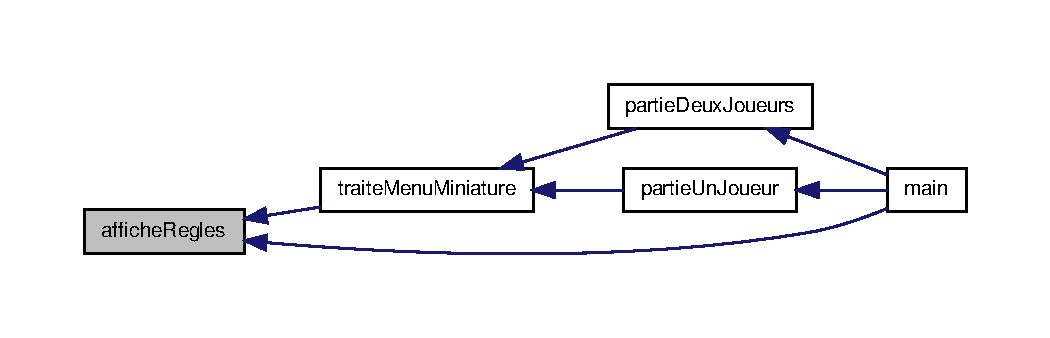
\includegraphics[width=350pt]{fonctions_affichage_8h_ad5c598ce2c6742ec4c3e771488987abe_icgraph}
\end{center}
\end{figure}


\hypertarget{fonctions_affichage_8h_aefaab0a4a9e4ccb284e6ce210fb6973b}{\index{fonctions\-Affichage.\-h@{fonctions\-Affichage.\-h}!choix\-Menu@{choix\-Menu}}
\index{choix\-Menu@{choix\-Menu}!fonctionsAffichage.h@{fonctions\-Affichage.\-h}}
\subsubsection[{choix\-Menu}]{\setlength{\rightskip}{0pt plus 5cm}short {\bf choix\-Menu} (
\begin{DoxyParamCaption}
\item[{int}]{abs\-Clic, }
\item[{int}]{ord\-Clic, }
\item[{\-S\-D\-L\-\_\-\-Rect}]{pos\-Tab\-Choix\-Menu\mbox{[}$\,$\mbox{]}}
\end{DoxyParamCaption}
)}}\label{fonctions_affichage_8h_aefaab0a4a9e4ccb284e6ce210fb6973b}


détermine si le joueur clique sur un des choix du menu 


\begin{DoxyParams}{\-Paramètres}
{\em abs\-Clic} & l'abscice du clic à traiter \\
\hline
{\em ord\-Clic} & l'ordonee du clic à traiter \\
\hline
{\em pos\-Tab\-Choix\-Menu} & \-Le tableau des position des item à traiter\\
\hline
\end{DoxyParams}
\begin{DoxyReturn}{\-Renvoie}
un nombre qui determnie un choix du menu 
\end{DoxyReturn}


\-Voici le graphe des appelants de cette fonction \-:
\nopagebreak
\begin{figure}[H]
\begin{center}
\leavevmode
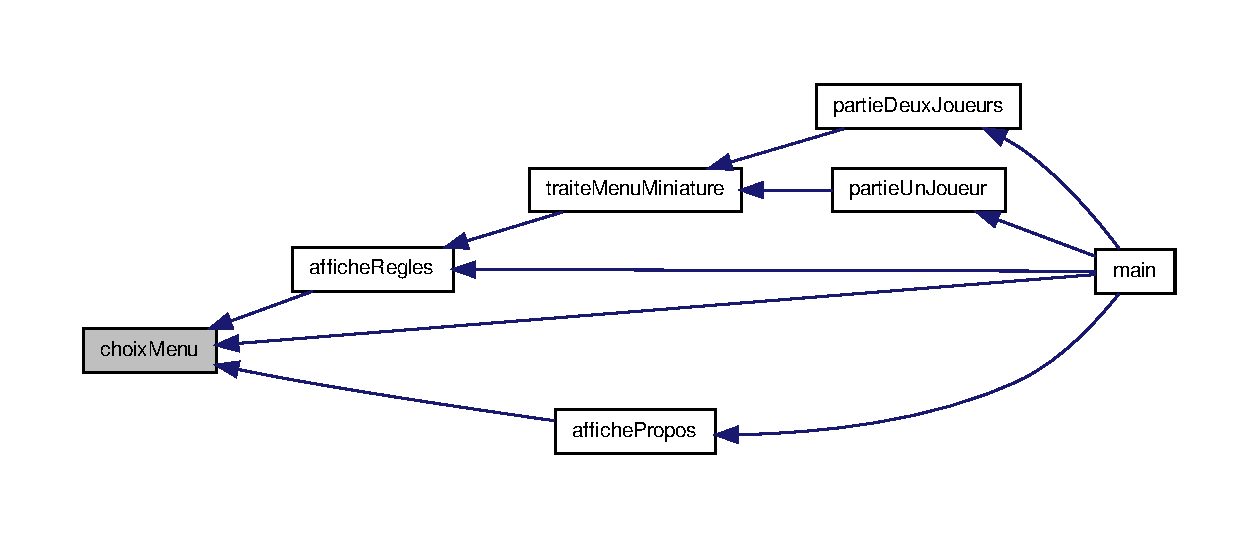
\includegraphics[width=350pt]{fonctions_affichage_8h_aefaab0a4a9e4ccb284e6ce210fb6973b_icgraph}
\end{center}
\end{figure}


\hypertarget{fonctions_affichage_8h_aa0b97452ac0e386637b196b6b8105c7d}{\index{fonctions\-Affichage.\-h@{fonctions\-Affichage.\-h}!init\-Menu\-Miniature@{init\-Menu\-Miniature}}
\index{init\-Menu\-Miniature@{init\-Menu\-Miniature}!fonctionsAffichage.h@{fonctions\-Affichage.\-h}}
\subsubsection[{init\-Menu\-Miniature}]{\setlength{\rightskip}{0pt plus 5cm}void {\bf init\-Menu\-Miniature} (
\begin{DoxyParamCaption}
\item[{int}]{partie, }
\item[{\-S\-D\-L\-\_\-\-Surface $\ast$}]{tab\-Menu\-Miniature\mbox{[}$\,$\mbox{]}, }
\item[{\-T\-T\-F\-\_\-\-Font $\ast$}]{police, }
\item[{\-S\-D\-L\-\_\-\-Color}]{couleur}
\end{DoxyParamCaption}
)}}\label{fonctions_affichage_8h_aa0b97452ac0e386637b196b6b8105c7d}


initialise le menu miniature selon la partie joué 


\begin{DoxyParams}{\-Paramètres}
{\em partie} & nombre servant à savoir si on joue à 1 ou 2 joueurs \\
\hline
{\em tab\-Menu\-Miniature\mbox{[}$\,$\mbox{]}} & \-Surface contenant les item du menu \\
\hline
{\em police} & la police utilisé \\
\hline
{\em couleur} & la couleur de la police \\
\hline
\end{DoxyParams}


\-Voici le graphe des appelants de cette fonction \-:
\nopagebreak
\begin{figure}[H]
\begin{center}
\leavevmode
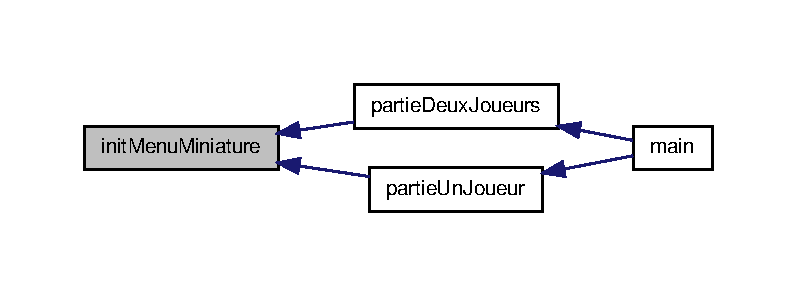
\includegraphics[width=350pt]{fonctions_affichage_8h_aa0b97452ac0e386637b196b6b8105c7d_icgraph}
\end{center}
\end{figure}


\hypertarget{fonctions_affichage_8h_a48262da5b852d7d777c20285f2f0b99a}{\index{fonctions\-Affichage.\-h@{fonctions\-Affichage.\-h}!traite\-Menu\-Miniature@{traite\-Menu\-Miniature}}
\index{traite\-Menu\-Miniature@{traite\-Menu\-Miniature}!fonctionsAffichage.h@{fonctions\-Affichage.\-h}}
\subsubsection[{traite\-Menu\-Miniature}]{\setlength{\rightskip}{0pt plus 5cm}short {\bf traite\-Menu\-Miniature} (
\begin{DoxyParamCaption}
\item[{int}]{abs\-Clic, }
\item[{int}]{ord\-Clic, }
\item[{\-S\-D\-L\-\_\-\-Surface $\ast$}]{ecran, }
\item[{int}]{partie}
\end{DoxyParamCaption}
)}}\label{fonctions_affichage_8h_a48262da5b852d7d777c20285f2f0b99a}


détermine si le joueur clique sur un des item du menu miniature 


\begin{DoxyParams}{\-Paramètres}
{\em abs\-Clic} & l'abscice du clic à traiter \\
\hline
{\em ord\-Clic} & l'ordonee du clic à traiter \\
\hline
{\em ecran} & la surface \-S\-D\-L où afficher les règles \\
\hline
{\em partie} & nombre servant à savoir si on joue à 1 ou 2 joueurs\\
\hline
\end{DoxyParams}
\begin{DoxyReturn}{\-Renvoie}
un nombre qui determine un choix du menu 
\end{DoxyReturn}


\-Voici le graphe d'appel pour cette fonction \-:
\nopagebreak
\begin{figure}[H]
\begin{center}
\leavevmode
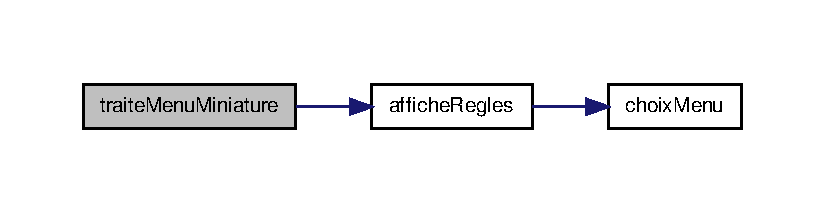
\includegraphics[width=350pt]{fonctions_affichage_8h_a48262da5b852d7d777c20285f2f0b99a_cgraph}
\end{center}
\end{figure}




\-Voici le graphe des appelants de cette fonction \-:
\nopagebreak
\begin{figure}[H]
\begin{center}
\leavevmode
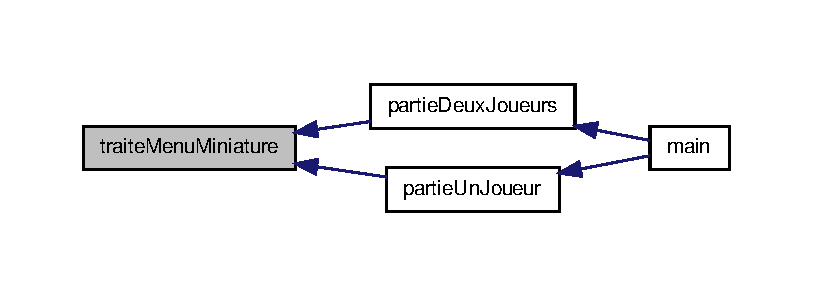
\includegraphics[width=350pt]{fonctions_affichage_8h_a48262da5b852d7d777c20285f2f0b99a_icgraph}
\end{center}
\end{figure}



\hypertarget{fonctions_i_a_8h}{\section{\-Référence du fichier headers/fonctions\-I\-A.h}
\label{fonctions_i_a_8h}\index{headers/fonctions\-I\-A.\-h@{headers/fonctions\-I\-A.\-h}}
}


définitions des prototypes des fonctions relatives à l'inteligence artificielle  


{\ttfamily \#include \char`\"{}constantes.\-h\char`\"{}}\*
\-Graphe des dépendances par inclusion de fonctions\-I\-A.\-h\-:
\nopagebreak
\begin{figure}[H]
\begin{center}
\leavevmode
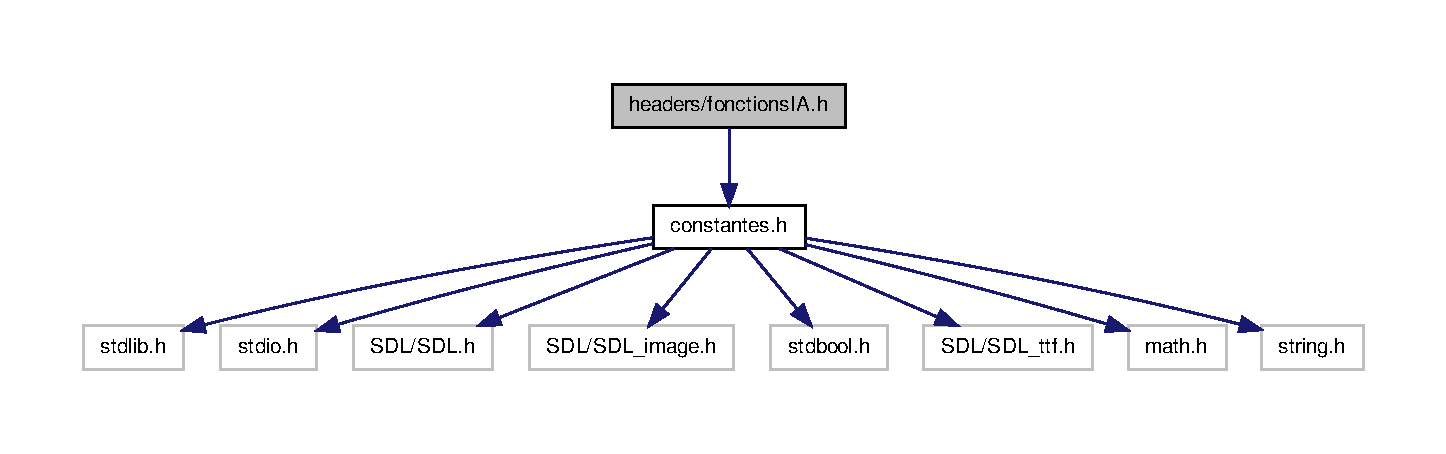
\includegraphics[width=350pt]{fonctions_i_a_8h__incl}
\end{center}
\end{figure}
\-Ce graphe montre quels fichiers incluent directement ou indirectement ce fichier \-:
\nopagebreak
\begin{figure}[H]
\begin{center}
\leavevmode
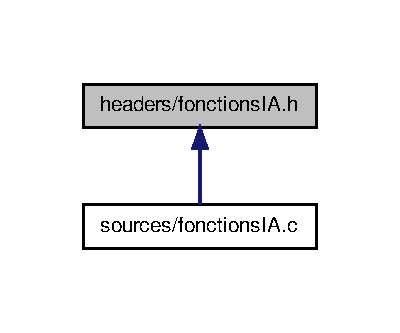
\includegraphics[width=192pt]{fonctions_i_a_8h__dep__incl}
\end{center}
\end{figure}
\subsection*{\-Structures de données}
\begin{DoxyCompactItemize}
\item 
struct \hyperlink{struct_coup}{\-Coup}
\begin{DoxyCompactList}\small\item\em indique un coup possible \end{DoxyCompactList}\end{DoxyCompactItemize}
\subsection*{\-Définitions de type}
\begin{DoxyCompactItemize}
\item 
\hypertarget{fonctions_i_a_8h_a9b046a9e4d0e97c49b4d51e7aa42fd66}{typedef struct \hyperlink{struct_coup}{\-Coup} {\bfseries \-Coup}}\label{fonctions_i_a_8h_a9b046a9e4d0e97c49b4d51e7aa42fd66}

\end{DoxyCompactItemize}
\subsection*{\-Fonctions}
\begin{DoxyCompactItemize}
\item 
short int \hyperlink{fonctions_i_a_8h_ae8b2b1efa750c376aeff3f38f665f76d}{evaluation\-Plateau} (\hyperlink{constantes_8h_ac19c17e9f0f0eeec3f3c11b052cfeb47}{\-Plateau} \-P)
\begin{DoxyCompactList}\small\item\em fonction evaluant si le plateau est plus ou moin favorable à l'ordi \end{DoxyCompactList}\item 
short int \hyperlink{fonctions_i_a_8h_a1416d179ad4f5765bbb790a77052b966}{alpha\-Beta} (\hyperlink{constantes_8h_ac19c17e9f0f0eeec3f3c11b052cfeb47}{\-Plateau} \-P, short int alpha, short int beta, short int profondeur)
\begin{DoxyCompactList}\small\item\em fonction recherchant le meilleur coup possible pour l'ordinateur en optimisant les passages dans l'arbre récursif \end{DoxyCompactList}\item 
short int \hyperlink{fonctions_i_a_8h_a8d45a9c590e7a75d0b34a4f61c4e9d0b}{calcul\-Gain} (\hyperlink{constantes_8h_ac19c17e9f0f0eeec3f3c11b052cfeb47}{\-Plateau} \-P, short int couleur\-Analyse)
\begin{DoxyCompactList}\small\item\em analyse le plateau pour une couleur \end{DoxyCompactList}\item 
bool \hyperlink{fonctions_i_a_8h_a395886ef8e187f1fcf83ec3dfba2caf9}{plateau\-Vide} (\hyperlink{constantes_8h_ac19c17e9f0f0eeec3f3c11b052cfeb47}{\-Plateau} \-P, int partie\-Tableau)
\begin{DoxyCompactList}\small\item\em determine si une partie de plateau est vide ou non \end{DoxyCompactList}\item 
void \hyperlink{fonctions_i_a_8h_a0e4cfe307082f42b29068d14fa592ccd}{meilleur\-Coup} (\hyperlink{constantes_8h_ac19c17e9f0f0eeec3f3c11b052cfeb47}{\-Plateau} \-P, short int couleur\-Analyse, \hyperlink{struct_coup}{\-Coup} $\ast$meilleur)
\begin{DoxyCompactList}\small\item\em détermine le meilleur coups potentiel à jouer par l'ia \end{DoxyCompactList}\end{DoxyCompactItemize}


\subsection{\-Description détaillée}
définitions des prototypes des fonctions relatives à l'inteligence artificielle 

\subsection{\-Documentation des fonctions}
\hypertarget{fonctions_i_a_8h_a1416d179ad4f5765bbb790a77052b966}{\index{fonctions\-I\-A.\-h@{fonctions\-I\-A.\-h}!alpha\-Beta@{alpha\-Beta}}
\index{alpha\-Beta@{alpha\-Beta}!fonctionsIA.h@{fonctions\-I\-A.\-h}}
\subsubsection[{alpha\-Beta}]{\setlength{\rightskip}{0pt plus 5cm}short int {\bf alpha\-Beta} (
\begin{DoxyParamCaption}
\item[{{\bf \-Plateau}}]{\-P, }
\item[{short int}]{alpha, }
\item[{short int}]{beta, }
\item[{short int}]{profondeur}
\end{DoxyParamCaption}
)}}\label{fonctions_i_a_8h_a1416d179ad4f5765bbb790a77052b966}


fonction recherchant le meilleur coup possible pour l'ordinateur en optimisant les passages dans l'arbre récursif 


\begin{DoxyParams}{\-Paramètres}
{\em \-P} & le plateau à évaluer \\
\hline
{\em alpha} & sert à la coupure dans les noeud max \\
\hline
{\em beta} & sert à la coupure dans les noeud min \\
\hline
{\em nombre\-\_\-coups} & pour la profondeur de l'arbre\\
\hline
\end{DoxyParams}
\begin{DoxyReturn}{\-Renvoie}
retourne le meilleur coup possible pour l'ordi 
\end{DoxyReturn}


\-Voici le graphe d'appel pour cette fonction \-:
\nopagebreak
\begin{figure}[H]
\begin{center}
\leavevmode
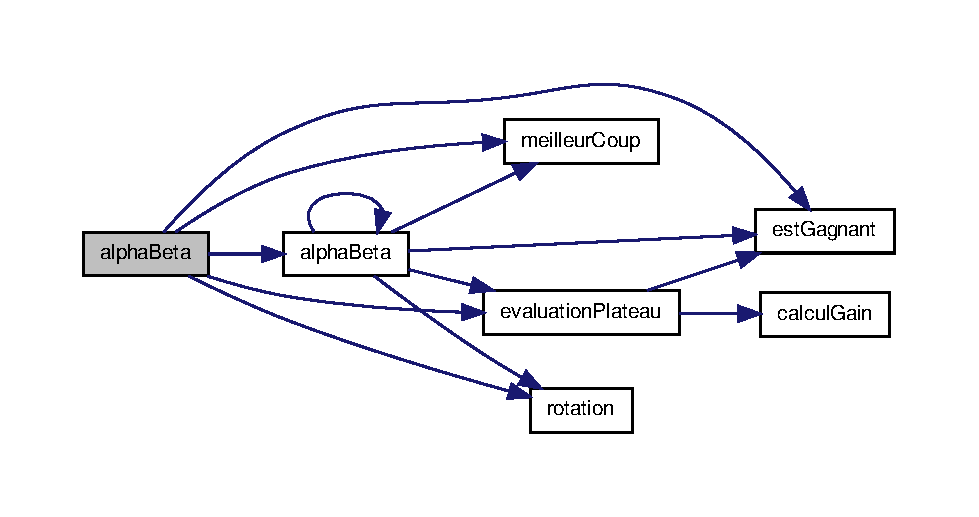
\includegraphics[width=350pt]{fonctions_i_a_8h_a1416d179ad4f5765bbb790a77052b966_cgraph}
\end{center}
\end{figure}




\-Voici le graphe des appelants de cette fonction \-:
\nopagebreak
\begin{figure}[H]
\begin{center}
\leavevmode
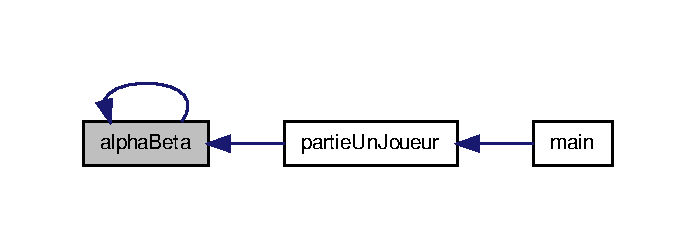
\includegraphics[width=334pt]{fonctions_i_a_8h_a1416d179ad4f5765bbb790a77052b966_icgraph}
\end{center}
\end{figure}


\hypertarget{fonctions_i_a_8h_a8d45a9c590e7a75d0b34a4f61c4e9d0b}{\index{fonctions\-I\-A.\-h@{fonctions\-I\-A.\-h}!calcul\-Gain@{calcul\-Gain}}
\index{calcul\-Gain@{calcul\-Gain}!fonctionsIA.h@{fonctions\-I\-A.\-h}}
\subsubsection[{calcul\-Gain}]{\setlength{\rightskip}{0pt plus 5cm}short int {\bf calcul\-Gain} (
\begin{DoxyParamCaption}
\item[{{\bf \-Plateau}}]{\-P, }
\item[{short int}]{couleur\-Analyse}
\end{DoxyParamCaption}
)}}\label{fonctions_i_a_8h_a8d45a9c590e7a75d0b34a4f61c4e9d0b}


analyse le plateau pour une couleur 

short int \hyperlink{fonctions_i_a_8h_a8d45a9c590e7a75d0b34a4f61c4e9d0b}{calcul\-Gain(\-Plateau P, short int couleur\-Analyse)} 
\begin{DoxyParams}{\-Paramètres}
{\em \-P} & le plateau à évaluer \\
\hline
{\em couleur\-Analyse} & represente la couleur à analyser \\
\hline
\end{DoxyParams}


\-Voici le graphe des appelants de cette fonction \-:
\nopagebreak
\begin{figure}[H]
\begin{center}
\leavevmode
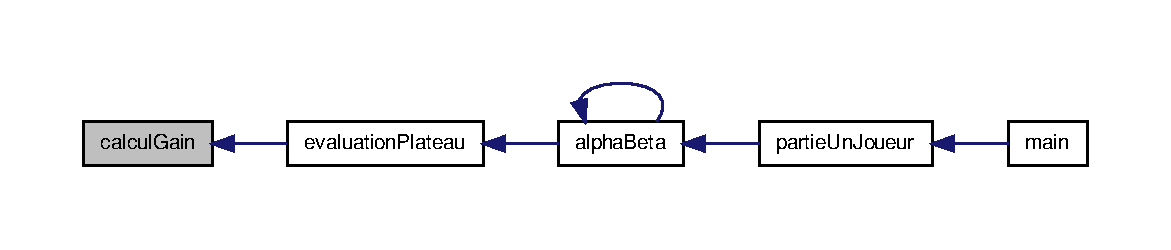
\includegraphics[width=350pt]{fonctions_i_a_8h_a8d45a9c590e7a75d0b34a4f61c4e9d0b_icgraph}
\end{center}
\end{figure}


\hypertarget{fonctions_i_a_8h_ae8b2b1efa750c376aeff3f38f665f76d}{\index{fonctions\-I\-A.\-h@{fonctions\-I\-A.\-h}!evaluation\-Plateau@{evaluation\-Plateau}}
\index{evaluation\-Plateau@{evaluation\-Plateau}!fonctionsIA.h@{fonctions\-I\-A.\-h}}
\subsubsection[{evaluation\-Plateau}]{\setlength{\rightskip}{0pt plus 5cm}short int {\bf evaluation\-Plateau} (
\begin{DoxyParamCaption}
\item[{{\bf \-Plateau}}]{\-P}
\end{DoxyParamCaption}
)}}\label{fonctions_i_a_8h_ae8b2b1efa750c376aeff3f38f665f76d}


fonction evaluant si le plateau est plus ou moin favorable à l'ordi 


\begin{DoxyParams}{\-Paramètres}
{\em \-P} & le plateau à évaluer\\
\hline
\end{DoxyParams}
\begin{DoxyReturn}{\-Renvoie}
un nombre qui représente le gain 
\end{DoxyReturn}


\-Voici le graphe d'appel pour cette fonction \-:
\nopagebreak
\begin{figure}[H]
\begin{center}
\leavevmode
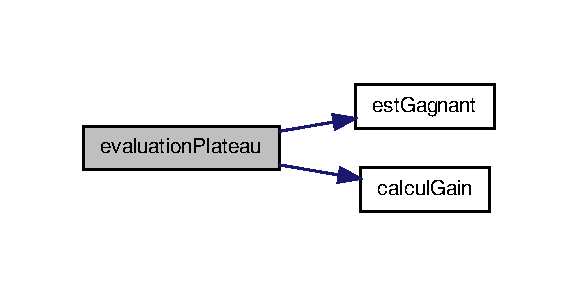
\includegraphics[width=278pt]{fonctions_i_a_8h_ae8b2b1efa750c376aeff3f38f665f76d_cgraph}
\end{center}
\end{figure}




\-Voici le graphe des appelants de cette fonction \-:
\nopagebreak
\begin{figure}[H]
\begin{center}
\leavevmode
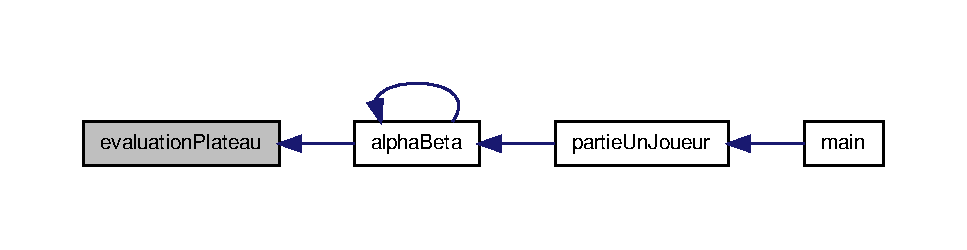
\includegraphics[width=350pt]{fonctions_i_a_8h_ae8b2b1efa750c376aeff3f38f665f76d_icgraph}
\end{center}
\end{figure}


\hypertarget{fonctions_i_a_8h_a0e4cfe307082f42b29068d14fa592ccd}{\index{fonctions\-I\-A.\-h@{fonctions\-I\-A.\-h}!meilleur\-Coup@{meilleur\-Coup}}
\index{meilleur\-Coup@{meilleur\-Coup}!fonctionsIA.h@{fonctions\-I\-A.\-h}}
\subsubsection[{meilleur\-Coup}]{\setlength{\rightskip}{0pt plus 5cm}void {\bf meilleur\-Coup} (
\begin{DoxyParamCaption}
\item[{{\bf \-Plateau}}]{\-P, }
\item[{short int}]{couleur\-Analyse, }
\item[{{\bf \-Coup} $\ast$}]{meilleur}
\end{DoxyParamCaption}
)}}\label{fonctions_i_a_8h_a0e4cfe307082f42b29068d14fa592ccd}


détermine le meilleur coups potentiel à jouer par l'ia 


\begin{DoxyParams}{\-Paramètres}
{\em \-P} & le plateau à évaluer \\
\hline
{\em couleur\-Analyse} & la couleur que l'on anamyse \\
\hline
{\em meilleur} & le meileur coup possible \\
\hline
\end{DoxyParams}


\-Voici le graphe des appelants de cette fonction \-:
\nopagebreak
\begin{figure}[H]
\begin{center}
\leavevmode
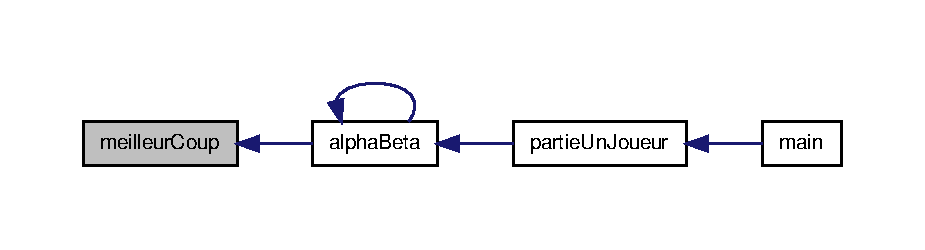
\includegraphics[width=350pt]{fonctions_i_a_8h_a0e4cfe307082f42b29068d14fa592ccd_icgraph}
\end{center}
\end{figure}


\hypertarget{fonctions_i_a_8h_a395886ef8e187f1fcf83ec3dfba2caf9}{\index{fonctions\-I\-A.\-h@{fonctions\-I\-A.\-h}!plateau\-Vide@{plateau\-Vide}}
\index{plateau\-Vide@{plateau\-Vide}!fonctionsIA.h@{fonctions\-I\-A.\-h}}
\subsubsection[{plateau\-Vide}]{\setlength{\rightskip}{0pt plus 5cm}bool {\bf plateau\-Vide} (
\begin{DoxyParamCaption}
\item[{{\bf \-Plateau}}]{\-P, }
\item[{int}]{partie\-Tableau}
\end{DoxyParamCaption}
)}}\label{fonctions_i_a_8h_a395886ef8e187f1fcf83ec3dfba2caf9}


determine si une partie de plateau est vide ou non 


\begin{DoxyParams}{\-Paramètres}
{\em \-P} & le plateau à évaluer \\
\hline
{\em partie\-Tableau} & nombre representant la partie du tablea \\
\hline
\end{DoxyParams}


\-Voici le graphe d'appel pour cette fonction \-:
\nopagebreak
\begin{figure}[H]
\begin{center}
\leavevmode
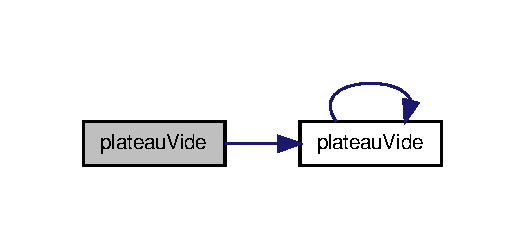
\includegraphics[width=252pt]{fonctions_i_a_8h_a395886ef8e187f1fcf83ec3dfba2caf9_cgraph}
\end{center}
\end{figure}




\-Voici le graphe des appelants de cette fonction \-:
\nopagebreak
\begin{figure}[H]
\begin{center}
\leavevmode
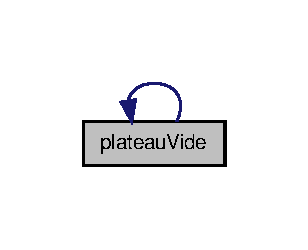
\includegraphics[width=148pt]{fonctions_i_a_8h_a395886ef8e187f1fcf83ec3dfba2caf9_icgraph}
\end{center}
\end{figure}



\hypertarget{fonctions_plateau_8h}{\section{\-Référence du fichier headers/fonctions\-Plateau.h}
\label{fonctions_plateau_8h}\index{headers/fonctions\-Plateau.\-h@{headers/fonctions\-Plateau.\-h}}
}


définitions des prototypes des fonctions relative au plateau  


{\ttfamily \#include \char`\"{}constantes.\-h\char`\"{}}\*
\-Graphe des dépendances par inclusion de fonctions\-Plateau.\-h\-:
\nopagebreak
\begin{figure}[H]
\begin{center}
\leavevmode
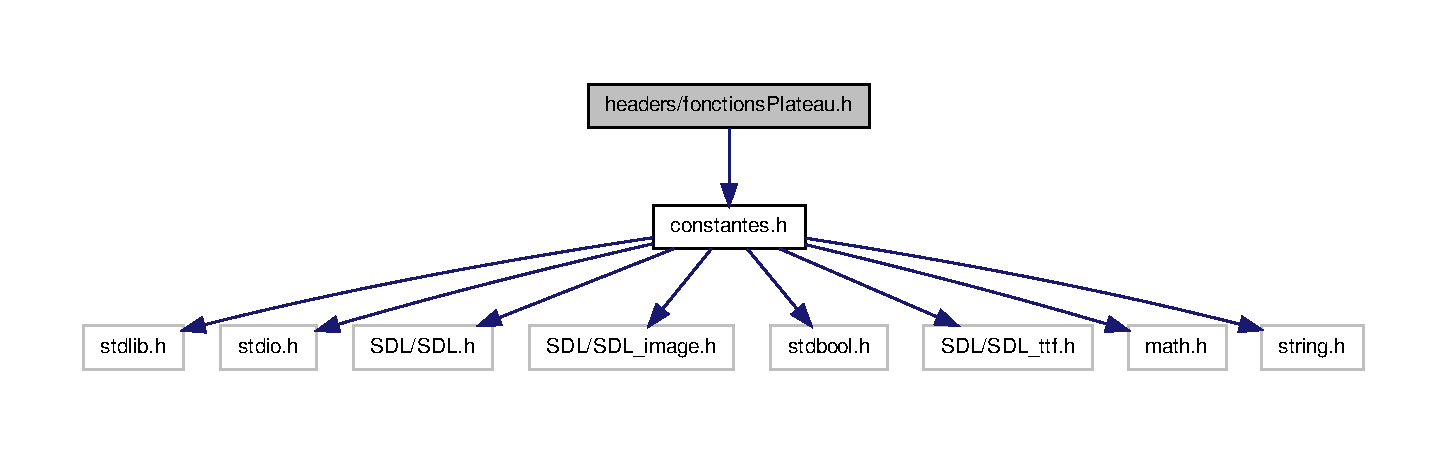
\includegraphics[width=350pt]{fonctions_plateau_8h__incl}
\end{center}
\end{figure}
\-Ce graphe montre quels fichiers incluent directement ou indirectement ce fichier \-:
\nopagebreak
\begin{figure}[H]
\begin{center}
\leavevmode
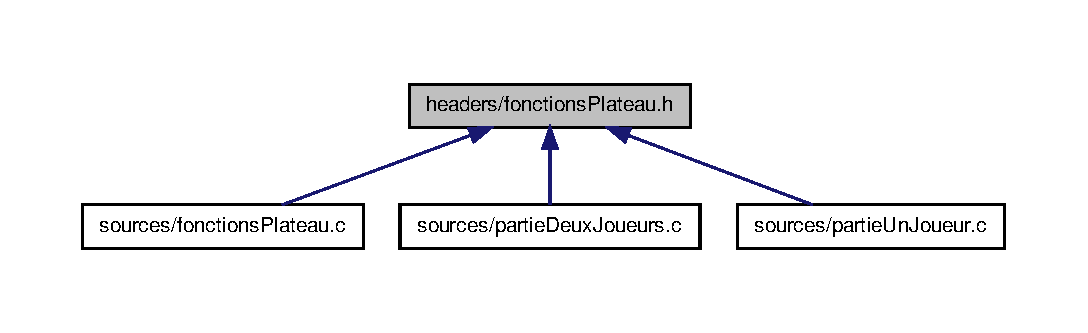
\includegraphics[width=350pt]{fonctions_plateau_8h__dep__incl}
\end{center}
\end{figure}
\subsection*{\-Structures de données}
\begin{DoxyCompactItemize}
\item 
struct \hyperlink{struct_input}{\-Input}
\begin{DoxyCompactList}\small\item\em sert à gerer les entréer saisis par le joueur \end{DoxyCompactList}\end{DoxyCompactItemize}
\subsection*{\-Fonctions}
\begin{DoxyCompactItemize}
\item 
void \hyperlink{fonctions_plateau_8h_aab348cdede8cfa4104aefc0dace18e05}{\-Update\-Events} (\hyperlink{struct_input}{\-Input} $\ast$in)
\begin{DoxyCompactList}\small\item\em gestion des events selon les entrées saisis \end{DoxyCompactList}\item 
void \hyperlink{fonctions_plateau_8h_af8c205efcbda1635fd2c62ce57b535b4}{init\-Plateau} (\hyperlink{constantes_8h_ac19c17e9f0f0eeec3f3c11b052cfeb47}{\-Plateau} \-P)
\begin{DoxyCompactList}\small\item\em initialisation du plateau de cases vides \end{DoxyCompactList}\item 
void \hyperlink{fonctions_plateau_8h_ae4dba04b9a0d5d145bafae6da91baca7}{affiche\-Plateau} (\-S\-D\-L\-\_\-\-Surface $\ast$ecran, \hyperlink{constantes_8h_ac19c17e9f0f0eeec3f3c11b052cfeb47}{\-Plateau} \-P, \-S\-D\-L\-\_\-\-Surface $\ast$tab\-Emplacement\-Bille\mbox{[}$\,$\mbox{]})
\begin{DoxyCompactList}\small\item\em affichage du plateau dans la fenetre \end{DoxyCompactList}\item 
bool \hyperlink{fonctions_plateau_8h_a95aaae34c0268305226854bb0ad1cff3}{placer\-Bille} (\hyperlink{constantes_8h_ac19c17e9f0f0eeec3f3c11b052cfeb47}{\-Plateau} \-P, int abs\-Clic, int ord\-Clic, int nombre\-\_\-coups)
\begin{DoxyCompactList}\small\item\em placement d'une bille sur un plateau \end{DoxyCompactList}\item 
bool \hyperlink{fonctions_plateau_8h_ac4c87ed6f29a02e05ccbc83097ff1f3c}{determiner\-Rotation} (int abs\-Clic, int ord\-Clic, \-S\-D\-L\-\_\-\-Rect tab\-Pos\-Fleche\-Rotation\mbox{[}$\,$\mbox{]}, int $\ast$\hyperlink{constantes_8h_aa65e3b592c27609a542733310b34f5d9}{sens}, int $\ast$partie\-Tableau)
\begin{DoxyCompactList}\small\item\em determiner quelle rotation il faut faire \end{DoxyCompactList}\item 
void \hyperlink{fonctions_plateau_8h_a8d7e72e320715fb45ec4e350b6d1f103}{rotation} (int \hyperlink{constantes_8h_ac19c17e9f0f0eeec3f3c11b052cfeb47}{\-Plateau}\mbox{[}$\,$\mbox{]}\mbox{[}\hyperlink{constantes_8h_abff55699e9fdf03f67a0279aa5c84ebe}{\-D\-I\-M\-\_\-\-P\-L\-A\-T\-E\-A\-U}\mbox{]}, int \hyperlink{constantes_8h_aa65e3b592c27609a542733310b34f5d9}{sens}, int partie\-Tableau)
\begin{DoxyCompactList}\small\item\em effectue une rotation sur un partie du plateau \end{DoxyCompactList}\item 
int \hyperlink{fonctions_plateau_8h_ab9d046b8743ee529bbeb780a0401241d}{est\-Gagnant} (int \hyperlink{constantes_8h_ac19c17e9f0f0eeec3f3c11b052cfeb47}{\-Plateau}\mbox{[}$\,$\mbox{]}\mbox{[}\hyperlink{constantes_8h_abff55699e9fdf03f67a0279aa5c84ebe}{\-D\-I\-M\-\_\-\-P\-L\-A\-T\-E\-A\-U}\mbox{]})
\begin{DoxyCompactList}\small\item\em determine si il y a un gagnant ou pas sur un plateau \end{DoxyCompactList}\end{DoxyCompactItemize}


\subsection{\-Description détaillée}
définitions des prototypes des fonctions relative au plateau 

\subsection{\-Documentation des fonctions}
\hypertarget{fonctions_plateau_8h_ae4dba04b9a0d5d145bafae6da91baca7}{\index{fonctions\-Plateau.\-h@{fonctions\-Plateau.\-h}!affiche\-Plateau@{affiche\-Plateau}}
\index{affiche\-Plateau@{affiche\-Plateau}!fonctionsPlateau.h@{fonctions\-Plateau.\-h}}
\subsubsection[{affiche\-Plateau}]{\setlength{\rightskip}{0pt plus 5cm}void {\bf affiche\-Plateau} (
\begin{DoxyParamCaption}
\item[{\-S\-D\-L\-\_\-\-Surface $\ast$}]{ecran, }
\item[{{\bf \-Plateau}}]{\-P, }
\item[{\-S\-D\-L\-\_\-\-Surface $\ast$}]{tab\-Emplacement\-Bille\mbox{[}$\,$\mbox{]}}
\end{DoxyParamCaption}
)}}\label{fonctions_plateau_8h_ae4dba04b9a0d5d145bafae6da91baca7}


affichage du plateau dans la fenetre 


\begin{DoxyParams}{\-Paramètres}
{\em ecran} & la surface \-S\-D\-L où afficher le plateau \\
\hline
{\em \-P} & le plateau à afficher \\
\hline
{\em tab\-Emplacement\-Bille\mbox{[}$\,$\mbox{]}} & tableau contenant les coordonnées de chaque bille \\
\hline
\end{DoxyParams}


\-Voici le graphe des appelants de cette fonction \-:
\nopagebreak
\begin{figure}[H]
\begin{center}
\leavevmode
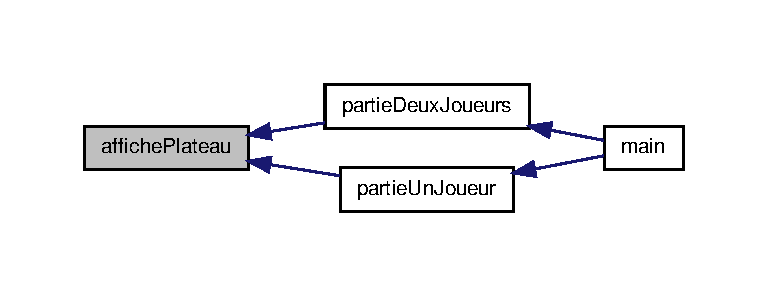
\includegraphics[width=350pt]{fonctions_plateau_8h_ae4dba04b9a0d5d145bafae6da91baca7_icgraph}
\end{center}
\end{figure}


\hypertarget{fonctions_plateau_8h_ac4c87ed6f29a02e05ccbc83097ff1f3c}{\index{fonctions\-Plateau.\-h@{fonctions\-Plateau.\-h}!determiner\-Rotation@{determiner\-Rotation}}
\index{determiner\-Rotation@{determiner\-Rotation}!fonctionsPlateau.h@{fonctions\-Plateau.\-h}}
\subsubsection[{determiner\-Rotation}]{\setlength{\rightskip}{0pt plus 5cm}bool {\bf determiner\-Rotation} (
\begin{DoxyParamCaption}
\item[{int}]{abs\-Clic, }
\item[{int}]{ord\-Clic, }
\item[{\-S\-D\-L\-\_\-\-Rect}]{tab\-Pos\-Fleche\-Rotation\mbox{[}$\,$\mbox{]}, }
\item[{int $\ast$}]{sens, }
\item[{int $\ast$}]{partie\-Tableau}
\end{DoxyParamCaption}
)}}\label{fonctions_plateau_8h_ac4c87ed6f29a02e05ccbc83097ff1f3c}


determiner quelle rotation il faut faire 


\begin{DoxyParams}{\-Paramètres}
{\em abs\-Clic} & abscice de la souris \\
\hline
{\em ord\-Clic} & ordonne de la souris \\
\hline
{\em tab\-Pos\-Fleche\-Rotation\mbox{[}$\,$\mbox{]}} & pour savoir la position des flèches a l'écran \\
\hline
{\em sens} & le sens de rotation a effectuer \\
\hline
{\em partie\-Tableau} & sur quelle partie du plateau on effectue la rotation\\
\hline
\end{DoxyParams}
\begin{DoxyReturn}{\-Renvoie}
vrais si on doit faire une rotation çàd si on a cliquer sur une flêche 
\end{DoxyReturn}


\-Voici le graphe des appelants de cette fonction \-:
\nopagebreak
\begin{figure}[H]
\begin{center}
\leavevmode
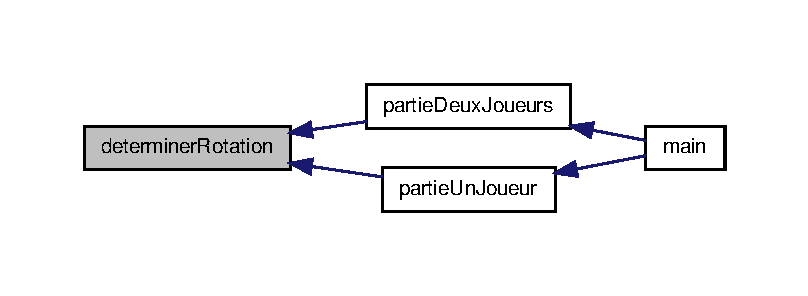
\includegraphics[width=350pt]{fonctions_plateau_8h_ac4c87ed6f29a02e05ccbc83097ff1f3c_icgraph}
\end{center}
\end{figure}


\hypertarget{fonctions_plateau_8h_ab9d046b8743ee529bbeb780a0401241d}{\index{fonctions\-Plateau.\-h@{fonctions\-Plateau.\-h}!est\-Gagnant@{est\-Gagnant}}
\index{est\-Gagnant@{est\-Gagnant}!fonctionsPlateau.h@{fonctions\-Plateau.\-h}}
\subsubsection[{est\-Gagnant}]{\setlength{\rightskip}{0pt plus 5cm}int {\bf est\-Gagnant} (
\begin{DoxyParamCaption}
\item[{int}]{\-Plateau\mbox{[}$\,$\mbox{]}\mbox{[}\-D\-I\-M\-\_\-\-P\-L\-A\-T\-E\-A\-U\mbox{]}}
\end{DoxyParamCaption}
)}}\label{fonctions_plateau_8h_ab9d046b8743ee529bbeb780a0401241d}


determine si il y a un gagnant ou pas sur un plateau 


\begin{DoxyParams}{\-Paramètres}
{\em le} & plateau analysé\\
\hline
\end{DoxyParams}
\begin{DoxyReturn}{\-Renvoie}
un nombre qui représente le gagnant 
\end{DoxyReturn}


\-Voici le graphe des appelants de cette fonction \-:
\nopagebreak
\begin{figure}[H]
\begin{center}
\leavevmode
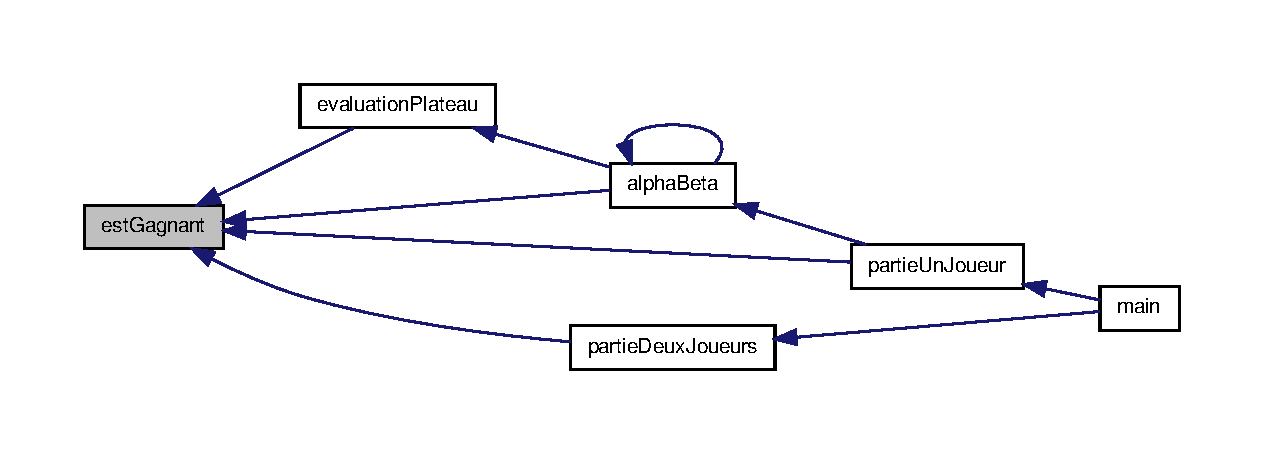
\includegraphics[width=350pt]{fonctions_plateau_8h_ab9d046b8743ee529bbeb780a0401241d_icgraph}
\end{center}
\end{figure}


\hypertarget{fonctions_plateau_8h_af8c205efcbda1635fd2c62ce57b535b4}{\index{fonctions\-Plateau.\-h@{fonctions\-Plateau.\-h}!init\-Plateau@{init\-Plateau}}
\index{init\-Plateau@{init\-Plateau}!fonctionsPlateau.h@{fonctions\-Plateau.\-h}}
\subsubsection[{init\-Plateau}]{\setlength{\rightskip}{0pt plus 5cm}void {\bf init\-Plateau} (
\begin{DoxyParamCaption}
\item[{{\bf \-Plateau}}]{\-P}
\end{DoxyParamCaption}
)}}\label{fonctions_plateau_8h_af8c205efcbda1635fd2c62ce57b535b4}


initialisation du plateau de cases vides 


\begin{DoxyParams}{\-Paramètres}
{\em \-P} & le plateau à initialiser \\
\hline
\end{DoxyParams}


\-Voici le graphe des appelants de cette fonction \-:
\nopagebreak
\begin{figure}[H]
\begin{center}
\leavevmode
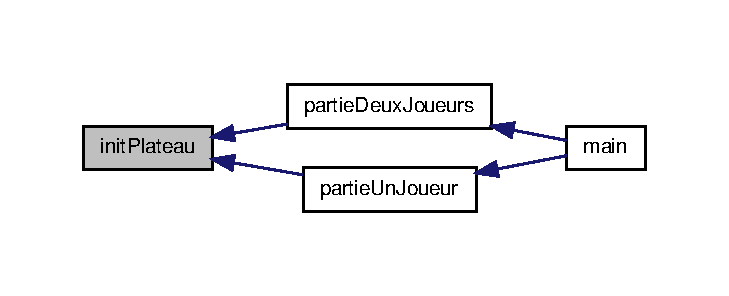
\includegraphics[width=350pt]{fonctions_plateau_8h_af8c205efcbda1635fd2c62ce57b535b4_icgraph}
\end{center}
\end{figure}


\hypertarget{fonctions_plateau_8h_a95aaae34c0268305226854bb0ad1cff3}{\index{fonctions\-Plateau.\-h@{fonctions\-Plateau.\-h}!placer\-Bille@{placer\-Bille}}
\index{placer\-Bille@{placer\-Bille}!fonctionsPlateau.h@{fonctions\-Plateau.\-h}}
\subsubsection[{placer\-Bille}]{\setlength{\rightskip}{0pt plus 5cm}bool {\bf placer\-Bille} (
\begin{DoxyParamCaption}
\item[{{\bf \-Plateau}}]{\-P, }
\item[{int}]{abs\-Clic, }
\item[{int}]{ord\-Clic, }
\item[{int}]{nbr\-\_\-coups}
\end{DoxyParamCaption}
)}}\label{fonctions_plateau_8h_a95aaae34c0268305226854bb0ad1cff3}


placement d'une bille sur un plateau 


\begin{DoxyParams}{\-Paramètres}
{\em \-P} & le plateau uitilisé \\
\hline
{\em abs\-Clic} & abscice de la souris \\
\hline
{\em ord\-Clic} & ordonne de la souris \\
\hline
{\em nombre\-\_\-coups} & nombre qui sert a determiner si on place une bille noire ou blanche\\
\hline
\end{DoxyParams}
\begin{DoxyReturn}{\-Renvoie}
vrais si une bille a été placée 
\end{DoxyReturn}


\-Voici le graphe des appelants de cette fonction \-:
\nopagebreak
\begin{figure}[H]
\begin{center}
\leavevmode
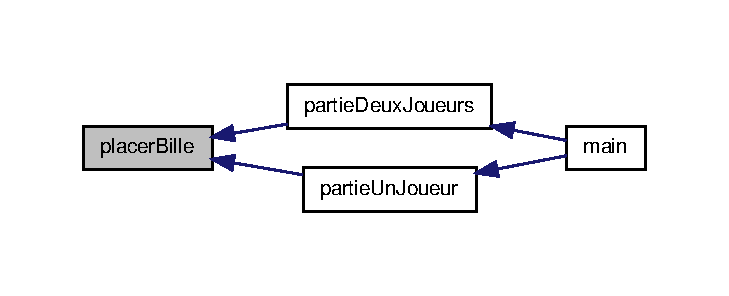
\includegraphics[width=350pt]{fonctions_plateau_8h_a95aaae34c0268305226854bb0ad1cff3_icgraph}
\end{center}
\end{figure}


\hypertarget{fonctions_plateau_8h_a8d7e72e320715fb45ec4e350b6d1f103}{\index{fonctions\-Plateau.\-h@{fonctions\-Plateau.\-h}!rotation@{rotation}}
\index{rotation@{rotation}!fonctionsPlateau.h@{fonctions\-Plateau.\-h}}
\subsubsection[{rotation}]{\setlength{\rightskip}{0pt plus 5cm}void {\bf rotation} (
\begin{DoxyParamCaption}
\item[{int}]{\-Plateau\mbox{[}$\,$\mbox{]}\mbox{[}\-D\-I\-M\-\_\-\-P\-L\-A\-T\-E\-A\-U\mbox{]}, }
\item[{int}]{sens, }
\item[{int}]{partie\-Tableau}
\end{DoxyParamCaption}
)}}\label{fonctions_plateau_8h_a8d7e72e320715fb45ec4e350b6d1f103}


effectue une rotation sur un partie du plateau 


\begin{DoxyParams}{\-Paramètres}
{\em \-Plateau} & le plateau utilisé \\
\hline
{\em sens} & le sens de la rotation \\
\hline
{\em partie\-Tableau} & la partie du plateau ou la rotation est effectuée \\
\hline
\end{DoxyParams}


\-Voici le graphe des appelants de cette fonction \-:
\nopagebreak
\begin{figure}[H]
\begin{center}
\leavevmode
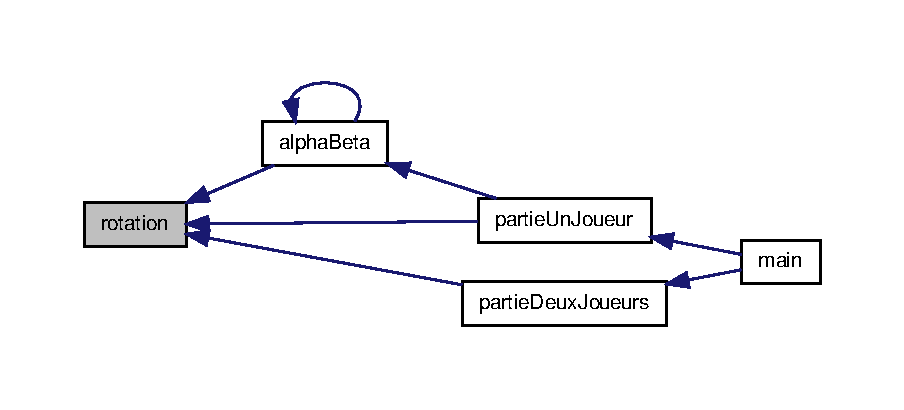
\includegraphics[width=350pt]{fonctions_plateau_8h_a8d7e72e320715fb45ec4e350b6d1f103_icgraph}
\end{center}
\end{figure}


\hypertarget{fonctions_plateau_8h_aab348cdede8cfa4104aefc0dace18e05}{\index{fonctions\-Plateau.\-h@{fonctions\-Plateau.\-h}!\-Update\-Events@{\-Update\-Events}}
\index{\-Update\-Events@{\-Update\-Events}!fonctionsPlateau.h@{fonctions\-Plateau.\-h}}
\subsubsection[{\-Update\-Events}]{\setlength{\rightskip}{0pt plus 5cm}void {\bf \-Update\-Events} (
\begin{DoxyParamCaption}
\item[{{\bf \-Input} $\ast$}]{in}
\end{DoxyParamCaption}
)}}\label{fonctions_plateau_8h_aab348cdede8cfa4104aefc0dace18e05}


gestion des events selon les entrées saisis 


\begin{DoxyParams}{\-Paramètres}
{\em in} & les entrées saisis \\
\hline
\end{DoxyParams}


\-Voici le graphe des appelants de cette fonction \-:
\nopagebreak
\begin{figure}[H]
\begin{center}
\leavevmode
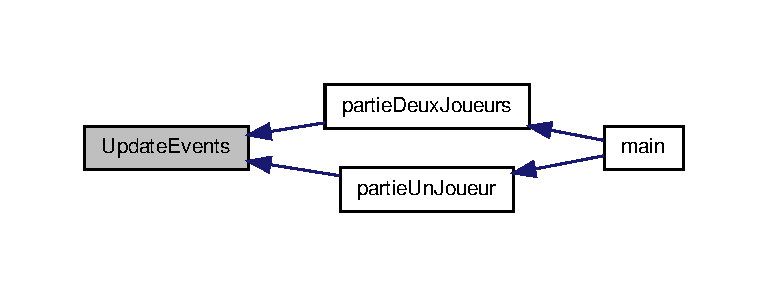
\includegraphics[width=350pt]{fonctions_plateau_8h_aab348cdede8cfa4104aefc0dace18e05_icgraph}
\end{center}
\end{figure}



\hypertarget{partie_deux_joueurs_8h}{\section{\-Référence du fichier headers/partie\-Deux\-Joueurs.h}
\label{partie_deux_joueurs_8h}\index{headers/partie\-Deux\-Joueurs.\-h@{headers/partie\-Deux\-Joueurs.\-h}}
}


définitions des prototypes des fonctions utilisé pour le mode 2 joueurs  


{\ttfamily \#include \char`\"{}constantes.\-h\char`\"{}}\*
\-Graphe des dépendances par inclusion de partie\-Deux\-Joueurs.\-h\-:
\nopagebreak
\begin{figure}[H]
\begin{center}
\leavevmode
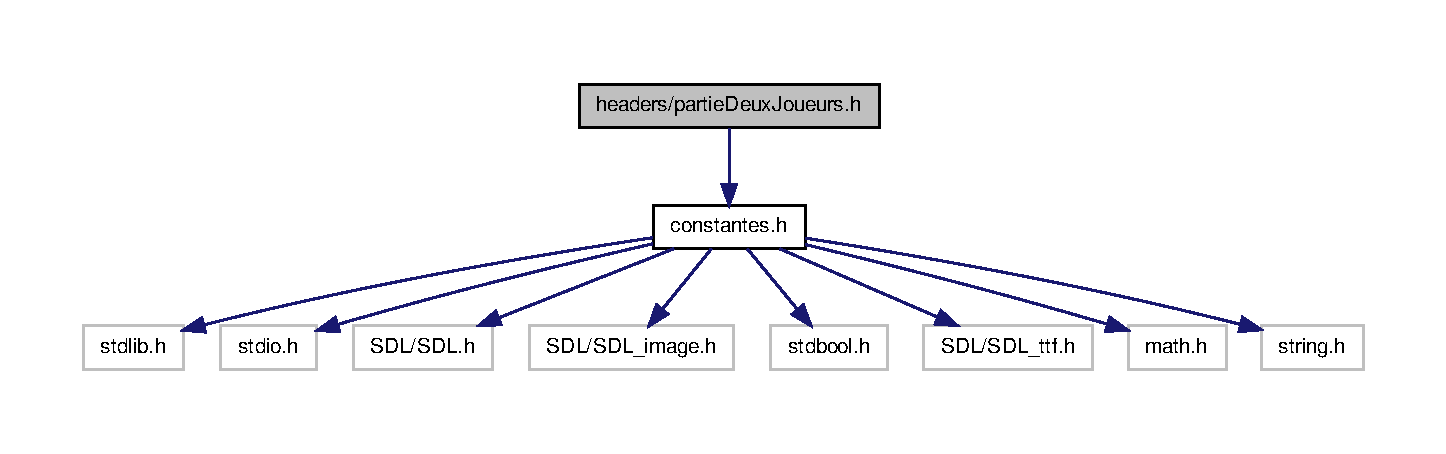
\includegraphics[width=350pt]{partie_deux_joueurs_8h__incl}
\end{center}
\end{figure}
\-Ce graphe montre quels fichiers incluent directement ou indirectement ce fichier \-:
\nopagebreak
\begin{figure}[H]
\begin{center}
\leavevmode
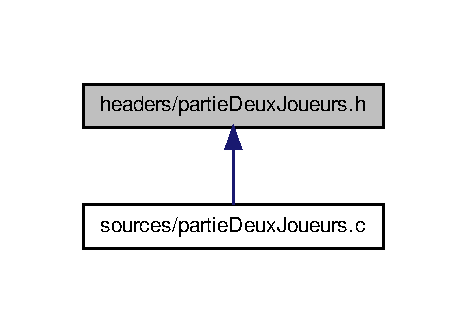
\includegraphics[width=224pt]{partie_deux_joueurs_8h__dep__incl}
\end{center}
\end{figure}
\subsection*{\-Fonctions}
\begin{DoxyCompactItemize}
\item 
int \hyperlink{partie_deux_joueurs_8h_a374909eadd0b6ee203667f93f32342ec}{partie\-Deux\-Joueurs} (\-S\-D\-L\-\_\-\-Surface $\ast$ecran)
\begin{DoxyCompactList}\small\item\em permet de jouer contre un joueur \end{DoxyCompactList}\end{DoxyCompactItemize}


\subsection{\-Description détaillée}
définitions des prototypes des fonctions utilisé pour le mode 2 joueurs 

\subsection{\-Documentation des fonctions}
\hypertarget{partie_deux_joueurs_8h_a374909eadd0b6ee203667f93f32342ec}{\index{partie\-Deux\-Joueurs.\-h@{partie\-Deux\-Joueurs.\-h}!partie\-Deux\-Joueurs@{partie\-Deux\-Joueurs}}
\index{partie\-Deux\-Joueurs@{partie\-Deux\-Joueurs}!partieDeuxJoueurs.h@{partie\-Deux\-Joueurs.\-h}}
\subsubsection[{partie\-Deux\-Joueurs}]{\setlength{\rightskip}{0pt plus 5cm}int {\bf partie\-Deux\-Joueurs} (
\begin{DoxyParamCaption}
\item[{\-S\-D\-L\-\_\-\-Surface $\ast$}]{ecran}
\end{DoxyParamCaption}
)}}\label{partie_deux_joueurs_8h_a374909eadd0b6ee203667f93f32342ec}


permet de jouer contre un joueur 


\begin{DoxyParams}{\-Paramètres}
{\em ecran} & affiche le jeu\\
\hline
\end{DoxyParams}
\begin{DoxyReturn}{\-Renvoie}
un nombre qui determine les actions de fin de jeu 
\end{DoxyReturn}


\-Voici le graphe d'appel pour cette fonction \-:
\nopagebreak
\begin{figure}[H]
\begin{center}
\leavevmode
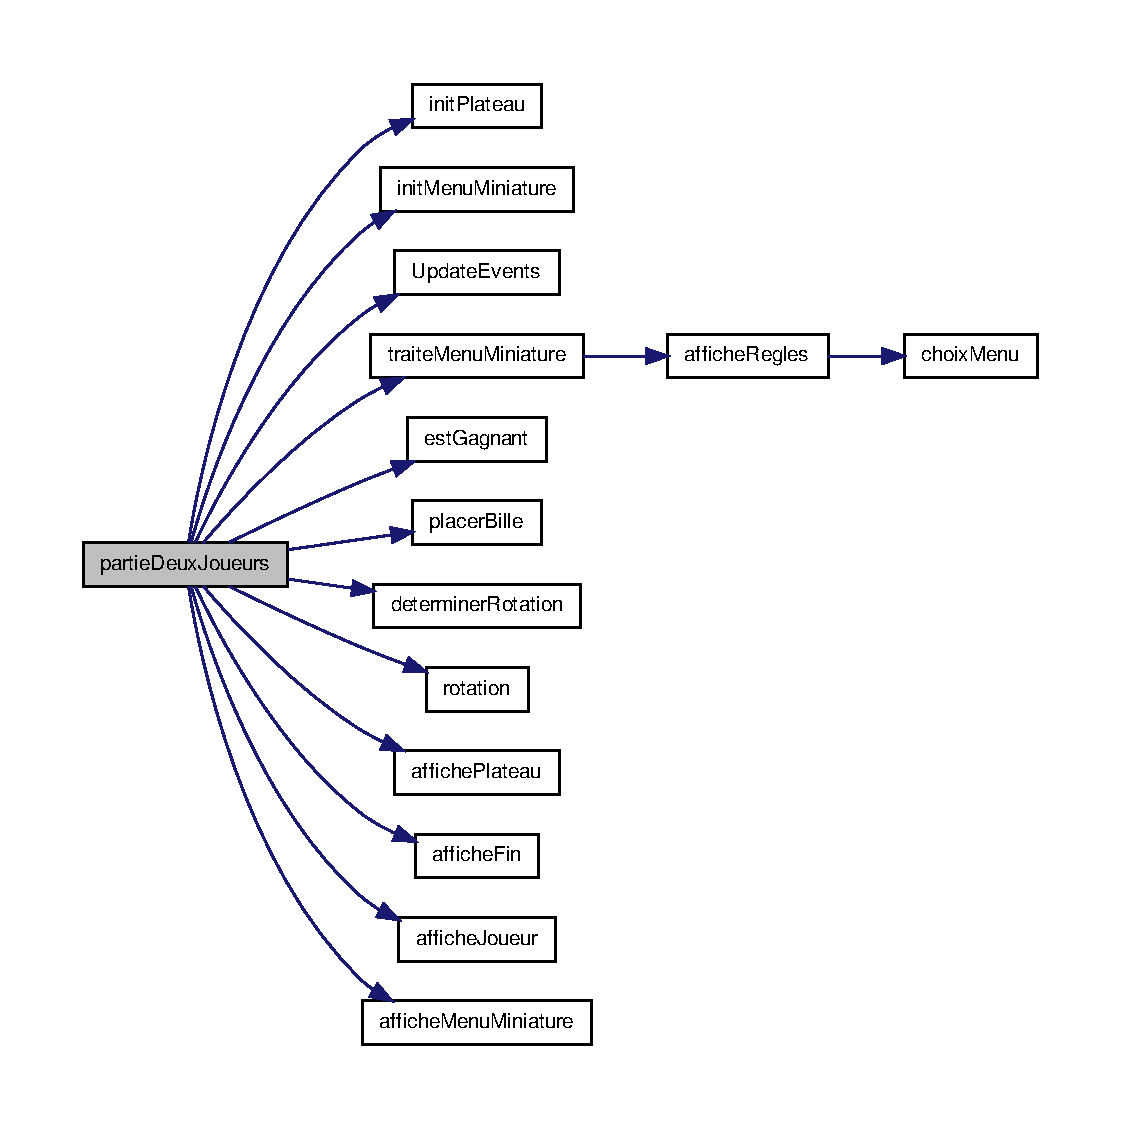
\includegraphics[width=350pt]{partie_deux_joueurs_8h_a374909eadd0b6ee203667f93f32342ec_cgraph}
\end{center}
\end{figure}




\-Voici le graphe des appelants de cette fonction \-:
\nopagebreak
\begin{figure}[H]
\begin{center}
\leavevmode
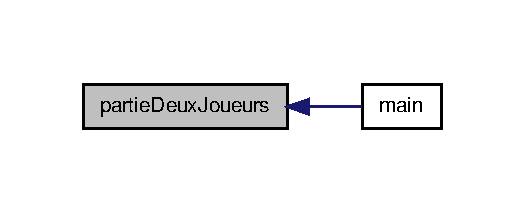
\includegraphics[width=252pt]{partie_deux_joueurs_8h_a374909eadd0b6ee203667f93f32342ec_icgraph}
\end{center}
\end{figure}



\hypertarget{partie_un_joueur_8h}{\section{\-Référence du fichier headers/partie\-Un\-Joueur.h}
\label{partie_un_joueur_8h}\index{headers/partie\-Un\-Joueur.\-h@{headers/partie\-Un\-Joueur.\-h}}
}


définitions des prototypes des fonctions utilisé pour le mode 1 joueurs  


{\ttfamily \#include \char`\"{}constantes.\-h\char`\"{}}\*
\-Graphe des dépendances par inclusion de partie\-Un\-Joueur.\-h\-:
\nopagebreak
\begin{figure}[H]
\begin{center}
\leavevmode
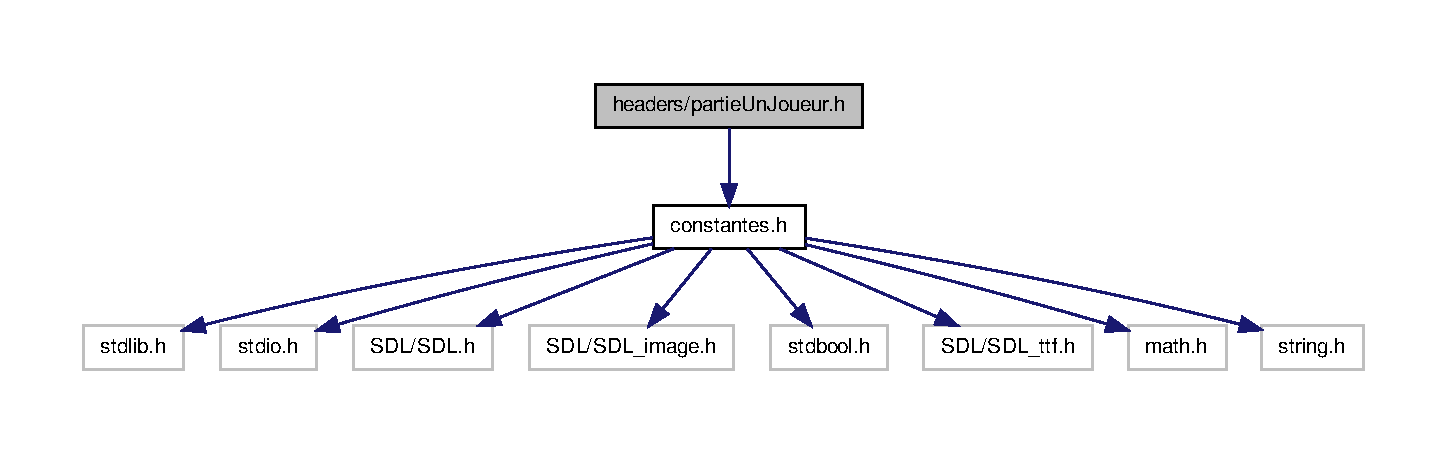
\includegraphics[width=350pt]{partie_un_joueur_8h__incl}
\end{center}
\end{figure}
\-Ce graphe montre quels fichiers incluent directement ou indirectement ce fichier \-:
\nopagebreak
\begin{figure}[H]
\begin{center}
\leavevmode
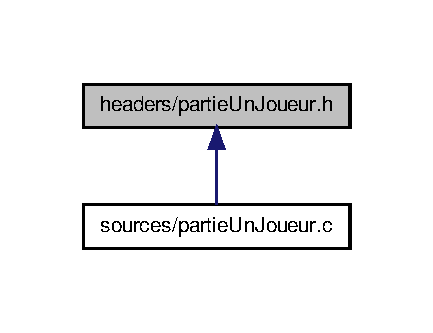
\includegraphics[width=208pt]{partie_un_joueur_8h__dep__incl}
\end{center}
\end{figure}
\subsection*{\-Fonctions}
\begin{DoxyCompactItemize}
\item 
int \hyperlink{partie_un_joueur_8h_a4abb180c273289e30fd8dd09696265f8}{partie\-Un\-Joueur} (\-S\-D\-L\-\_\-\-Surface $\ast$ecran)
\begin{DoxyCompactList}\small\item\em permet de jouer contre l'ordinateur \end{DoxyCompactList}\end{DoxyCompactItemize}


\subsection{\-Description détaillée}
définitions des prototypes des fonctions utilisé pour le mode 1 joueurs 

\subsection{\-Documentation des fonctions}
\hypertarget{partie_un_joueur_8h_a4abb180c273289e30fd8dd09696265f8}{\index{partie\-Un\-Joueur.\-h@{partie\-Un\-Joueur.\-h}!partie\-Un\-Joueur@{partie\-Un\-Joueur}}
\index{partie\-Un\-Joueur@{partie\-Un\-Joueur}!partieUnJoueur.h@{partie\-Un\-Joueur.\-h}}
\subsubsection[{partie\-Un\-Joueur}]{\setlength{\rightskip}{0pt plus 5cm}int {\bf partie\-Un\-Joueur} (
\begin{DoxyParamCaption}
\item[{\-S\-D\-L\-\_\-\-Surface $\ast$}]{ecran}
\end{DoxyParamCaption}
)}}\label{partie_un_joueur_8h_a4abb180c273289e30fd8dd09696265f8}


permet de jouer contre l'ordinateur 


\begin{DoxyParams}{\-Paramètres}
{\em ecran} & affiche le jeu\\
\hline
\end{DoxyParams}
\begin{DoxyReturn}{\-Renvoie}
un nombre qui determine les actions de fin de jeu 
\end{DoxyReturn}


\-Voici le graphe d'appel pour cette fonction \-:
\nopagebreak
\begin{figure}[H]
\begin{center}
\leavevmode
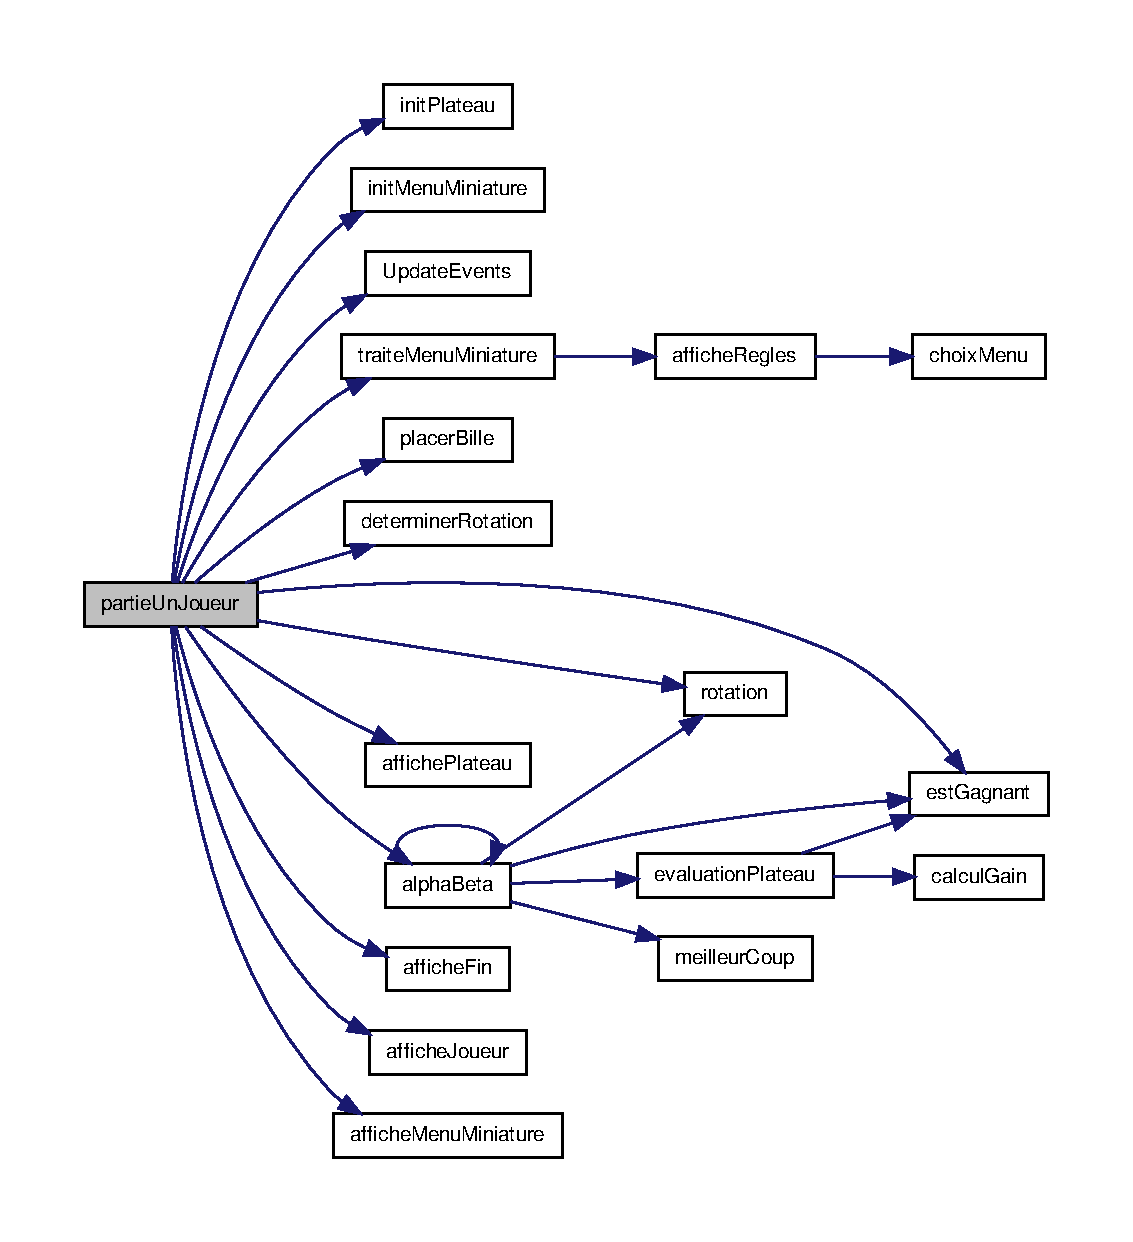
\includegraphics[width=350pt]{partie_un_joueur_8h_a4abb180c273289e30fd8dd09696265f8_cgraph}
\end{center}
\end{figure}




\-Voici le graphe des appelants de cette fonction \-:
\nopagebreak
\begin{figure}[H]
\begin{center}
\leavevmode
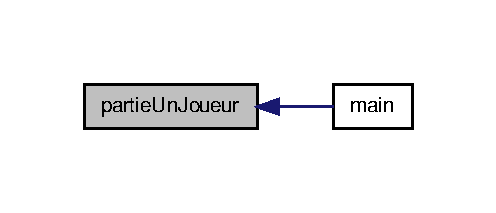
\includegraphics[width=238pt]{partie_un_joueur_8h_a4abb180c273289e30fd8dd09696265f8_icgraph}
\end{center}
\end{figure}



\hypertarget{fonctions_affichage_8c}{\section{\-Référence du fichier sources/fonctions\-Affichage.c}
\label{fonctions_affichage_8c}\index{sources/fonctions\-Affichage.\-c@{sources/fonctions\-Affichage.\-c}}
}


fonctions relatives à l'affichage et aux traitement des menus  


{\ttfamily \#include \char`\"{}../headers/fonctions\-Affichage.\-h\char`\"{}}\*
\-Graphe des dépendances par inclusion de fonctions\-Affichage.\-c\-:
\nopagebreak
\begin{figure}[H]
\begin{center}
\leavevmode
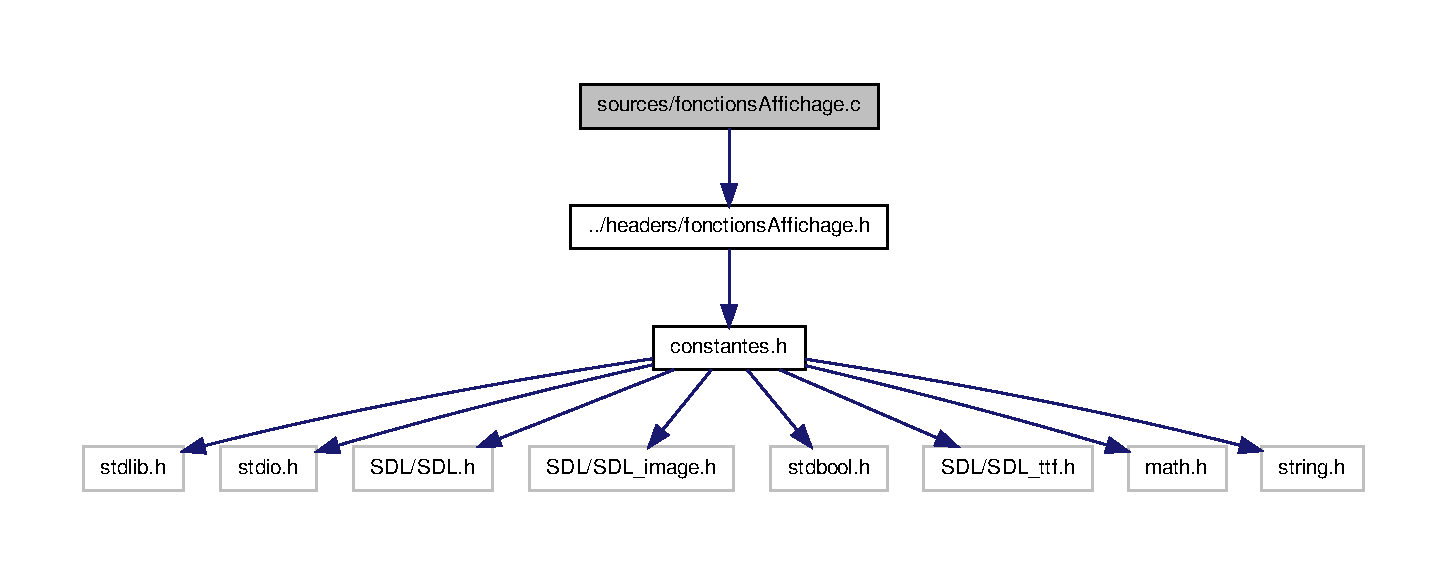
\includegraphics[width=350pt]{fonctions_affichage_8c__incl}
\end{center}
\end{figure}
\subsection*{\-Fonctions}
\begin{DoxyCompactItemize}
\item 
void \hyperlink{fonctions_affichage_8c_a6de5a4b9281294c56a4bd7254cdb481d}{affiche\-Fin} (int nom\-\_\-gagnant, int nombre\-\_\-coups, \-T\-T\-F\-\_\-\-Font $\ast$police, \-S\-D\-L\-\_\-\-Surface $\ast$texte, \-S\-D\-L\-\_\-\-Color couleur, \-S\-D\-L\-\_\-\-Surface $\ast$ecran)
\begin{DoxyCompactList}\small\item\em affiche quand une partie est terminée le nom du gagnant et le nombre de coup joué par celui ci \end{DoxyCompactList}\item 
short \hyperlink{fonctions_affichage_8c_a6a74e3ea603ed4022ce59f1e57dbb6dd}{affiche\-Regles} (\-S\-D\-L\-\_\-\-Surface $\ast$ecran)
\begin{DoxyCompactList}\small\item\em \-Affiche les rêgles du jeu. \end{DoxyCompactList}\item 
short \hyperlink{fonctions_affichage_8c_a830a6d65d1a989f174c3bcde5ae69151}{affiche\-Propos} (\-S\-D\-L\-\_\-\-Surface $\ast$ecran)
\begin{DoxyCompactList}\small\item\em \-Affiche les information sur le jeu. \end{DoxyCompactList}\item 
short \hyperlink{fonctions_affichage_8c_aefaab0a4a9e4ccb284e6ce210fb6973b}{choix\-Menu} (int abs\-Clic, int ord\-Clic, \-S\-D\-L\-\_\-\-Rect pos\-Tab\-Choix\-Menu\mbox{[}$\,$\mbox{]})
\begin{DoxyCompactList}\small\item\em détermine si le joueur clique sur un des choix du menu \end{DoxyCompactList}\item 
void \hyperlink{fonctions_affichage_8c_a805c8a6f72037e8a2d3649e1ff874fa0}{affiche\-Menu\-Miniature} (\-S\-D\-L\-\_\-\-Surface $\ast$ecran, \-S\-D\-L\-\_\-\-Surface $\ast$tab\-Menu\-Miniature\mbox{[}$\,$\mbox{]}, \-S\-D\-L\-\_\-\-Rect pos\-Tab\-Menu\-Miniature\mbox{[}$\,$\mbox{]})
\begin{DoxyCompactList}\small\item\em affiche le menu miniature situé en bas de la fenêtre \end{DoxyCompactList}\item 
short \hyperlink{fonctions_affichage_8c_a48262da5b852d7d777c20285f2f0b99a}{traite\-Menu\-Miniature} (int abs\-Clic, int ord\-Clic, \-S\-D\-L\-\_\-\-Surface $\ast$ecran, int partie)
\begin{DoxyCompactList}\small\item\em détermine si le joueur clique sur un des item du menu miniature \end{DoxyCompactList}\item 
void \hyperlink{fonctions_affichage_8c_aa0b97452ac0e386637b196b6b8105c7d}{init\-Menu\-Miniature} (int partie, \-S\-D\-L\-\_\-\-Surface $\ast$tab\-Menu\-Miniature\mbox{[}$\,$\mbox{]}, \-T\-T\-F\-\_\-\-Font $\ast$police, \-S\-D\-L\-\_\-\-Color couleur)
\begin{DoxyCompactList}\small\item\em initialise le menu miniature selon la partie joué \end{DoxyCompactList}\item 
void \hyperlink{fonctions_affichage_8c_a6cede375026585c570c284965c06f83a}{affiche\-Joueur} (\-S\-D\-L\-\_\-\-Surface $\ast$ecran, int nb\-\_\-coups, \-T\-T\-F\-\_\-\-Font $\ast$police, \-S\-D\-L\-\_\-\-Color couleur)
\begin{DoxyCompactList}\small\item\em fonction affichant le joueur qui est en train de jouer \end{DoxyCompactList}\end{DoxyCompactItemize}


\subsection{\-Description détaillée}
fonctions relatives à l'affichage et aux traitement des menus 

\subsection{\-Documentation des fonctions}
\hypertarget{fonctions_affichage_8c_a6de5a4b9281294c56a4bd7254cdb481d}{\index{fonctions\-Affichage.\-c@{fonctions\-Affichage.\-c}!affiche\-Fin@{affiche\-Fin}}
\index{affiche\-Fin@{affiche\-Fin}!fonctionsAffichage.c@{fonctions\-Affichage.\-c}}
\subsubsection[{affiche\-Fin}]{\setlength{\rightskip}{0pt plus 5cm}void {\bf affiche\-Fin} (
\begin{DoxyParamCaption}
\item[{int}]{nom\-\_\-gagnant, }
\item[{int}]{nombre\-\_\-coups, }
\item[{\-T\-T\-F\-\_\-\-Font $\ast$}]{police, }
\item[{\-S\-D\-L\-\_\-\-Surface $\ast$}]{texte, }
\item[{\-S\-D\-L\-\_\-\-Color}]{couleur, }
\item[{\-S\-D\-L\-\_\-\-Surface $\ast$}]{ecran}
\end{DoxyParamCaption}
)}}\label{fonctions_affichage_8c_a6de5a4b9281294c56a4bd7254cdb481d}


affiche quand une partie est terminée le nom du gagnant et le nombre de coup joué par celui ci 


\begin{DoxyParams}{\-Paramètres}
{\em nom\-\_\-gagnant} & le nom du gagnant conforme à l'énumération gagnant \\
\hline
{\em nombre\-\_\-coups} & le nombre de coups joué par un joueur \\
\hline
{\em police} & la police qui sert à écrire les informations \\
\hline
{\em texte} & la \-S\-D\-L\-\_\-\-Surface sur laquelle on affiche les informations \\
\hline
{\em couleur} & la couleur de la police \\
\hline
{\em ecran} & la surface \-S\-D\-L où afficher la fin \\
\hline
\end{DoxyParams}


\-Voici le graphe des appelants de cette fonction \-:
\nopagebreak
\begin{figure}[H]
\begin{center}
\leavevmode
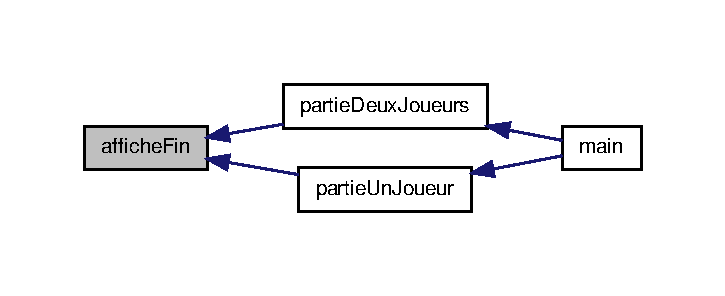
\includegraphics[width=348pt]{fonctions_affichage_8c_a6de5a4b9281294c56a4bd7254cdb481d_icgraph}
\end{center}
\end{figure}


\hypertarget{fonctions_affichage_8c_a6cede375026585c570c284965c06f83a}{\index{fonctions\-Affichage.\-c@{fonctions\-Affichage.\-c}!affiche\-Joueur@{affiche\-Joueur}}
\index{affiche\-Joueur@{affiche\-Joueur}!fonctionsAffichage.c@{fonctions\-Affichage.\-c}}
\subsubsection[{affiche\-Joueur}]{\setlength{\rightskip}{0pt plus 5cm}void {\bf affiche\-Joueur} (
\begin{DoxyParamCaption}
\item[{\-S\-D\-L\-\_\-\-Surface $\ast$}]{ecran, }
\item[{int}]{nb\-\_\-coups, }
\item[{\-T\-T\-F\-\_\-\-Font $\ast$}]{police, }
\item[{\-S\-D\-L\-\_\-\-Color}]{couleur}
\end{DoxyParamCaption}
)}}\label{fonctions_affichage_8c_a6cede375026585c570c284965c06f83a}


fonction affichant le joueur qui est en train de jouer 


\begin{DoxyParams}{\-Paramètres}
{\em ecran} & la surface \-S\-D\-L où afficher le joueur \\
\hline
{\em nb\-\_\-coups} & nombre qui nous sert a determiner le joueur courant selon le nombre de coups joué \\
\hline
{\em police} & la police utilisé \\
\hline
{\em couleur} & la couleur de la police \\
\hline
\end{DoxyParams}


\-Voici le graphe des appelants de cette fonction \-:
\nopagebreak
\begin{figure}[H]
\begin{center}
\leavevmode
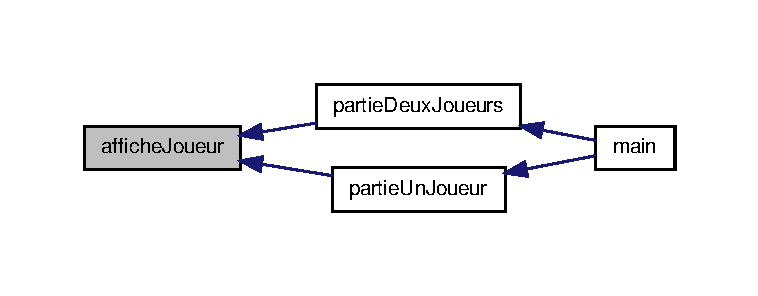
\includegraphics[width=350pt]{fonctions_affichage_8c_a6cede375026585c570c284965c06f83a_icgraph}
\end{center}
\end{figure}


\hypertarget{fonctions_affichage_8c_a805c8a6f72037e8a2d3649e1ff874fa0}{\index{fonctions\-Affichage.\-c@{fonctions\-Affichage.\-c}!affiche\-Menu\-Miniature@{affiche\-Menu\-Miniature}}
\index{affiche\-Menu\-Miniature@{affiche\-Menu\-Miniature}!fonctionsAffichage.c@{fonctions\-Affichage.\-c}}
\subsubsection[{affiche\-Menu\-Miniature}]{\setlength{\rightskip}{0pt plus 5cm}void {\bf affiche\-Menu\-Miniature} (
\begin{DoxyParamCaption}
\item[{\-S\-D\-L\-\_\-\-Surface $\ast$}]{ecran, }
\item[{\-S\-D\-L\-\_\-\-Surface $\ast$}]{tab\-Menu\-Miniature\mbox{[}$\,$\mbox{]}, }
\item[{\-S\-D\-L\-\_\-\-Rect}]{pos\-Tab\-Menu\-Miniature\mbox{[}$\,$\mbox{]}}
\end{DoxyParamCaption}
)}}\label{fonctions_affichage_8c_a805c8a6f72037e8a2d3649e1ff874fa0}


affiche le menu miniature situé en bas de la fenêtre 


\begin{DoxyParams}{\-Paramètres}
{\em ecran} & la surface \-S\-D\-L où afficher le menu miniature \\
\hline
{\em tab\-Menu\-Miniature\mbox{[}$\,$\mbox{]}} & tableau contenant les élément du menu miniature \\
\hline
{\em postab\-Menu\-Miniature\mbox{[}$\,$\mbox{]}} & tableau contenant la position des élément du menu miniature \\
\hline
\end{DoxyParams}


\-Voici le graphe des appelants de cette fonction \-:
\nopagebreak
\begin{figure}[H]
\begin{center}
\leavevmode
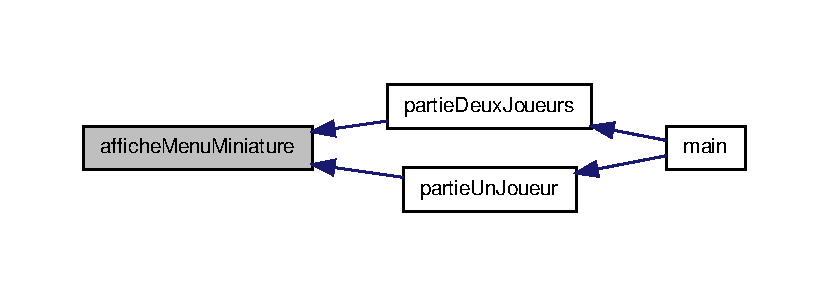
\includegraphics[width=350pt]{fonctions_affichage_8c_a805c8a6f72037e8a2d3649e1ff874fa0_icgraph}
\end{center}
\end{figure}


\hypertarget{fonctions_affichage_8c_a830a6d65d1a989f174c3bcde5ae69151}{\index{fonctions\-Affichage.\-c@{fonctions\-Affichage.\-c}!affiche\-Propos@{affiche\-Propos}}
\index{affiche\-Propos@{affiche\-Propos}!fonctionsAffichage.c@{fonctions\-Affichage.\-c}}
\subsubsection[{affiche\-Propos}]{\setlength{\rightskip}{0pt plus 5cm}short {\bf affiche\-Propos} (
\begin{DoxyParamCaption}
\item[{\-S\-D\-L\-\_\-\-Surface $\ast$}]{ecran}
\end{DoxyParamCaption}
)}}\label{fonctions_affichage_8c_a830a6d65d1a989f174c3bcde5ae69151}


\-Affiche les information sur le jeu. 


\begin{DoxyParams}{\-Paramètres}
{\em ecran} & la surface \-S\-D\-L où afficher les informations\\
\hline
\end{DoxyParams}
\begin{DoxyReturn}{\-Renvoie}
retourne \-E\-X\-I\-T\-\_\-\-S\-U\-C\-C\-E\-S\-S pour verifier si la fonction c'est exécuté normalement 
\end{DoxyReturn}


\-Voici le graphe d'appel pour cette fonction \-:
\nopagebreak
\begin{figure}[H]
\begin{center}
\leavevmode
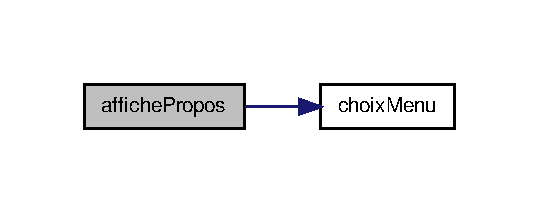
\includegraphics[width=258pt]{fonctions_affichage_8c_a830a6d65d1a989f174c3bcde5ae69151_cgraph}
\end{center}
\end{figure}




\-Voici le graphe des appelants de cette fonction \-:
\nopagebreak
\begin{figure}[H]
\begin{center}
\leavevmode
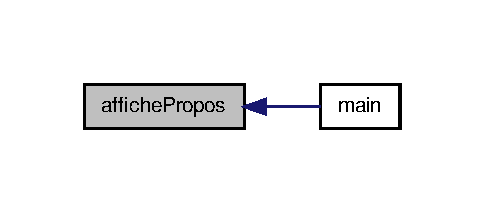
\includegraphics[width=232pt]{fonctions_affichage_8c_a830a6d65d1a989f174c3bcde5ae69151_icgraph}
\end{center}
\end{figure}


\hypertarget{fonctions_affichage_8c_a6a74e3ea603ed4022ce59f1e57dbb6dd}{\index{fonctions\-Affichage.\-c@{fonctions\-Affichage.\-c}!affiche\-Regles@{affiche\-Regles}}
\index{affiche\-Regles@{affiche\-Regles}!fonctionsAffichage.c@{fonctions\-Affichage.\-c}}
\subsubsection[{affiche\-Regles}]{\setlength{\rightskip}{0pt plus 5cm}void {\bf affiche\-Regles} (
\begin{DoxyParamCaption}
\item[{\-S\-D\-L\-\_\-\-Surface $\ast$}]{ecran}
\end{DoxyParamCaption}
)}}\label{fonctions_affichage_8c_a6a74e3ea603ed4022ce59f1e57dbb6dd}


\-Affiche les rêgles du jeu. 


\begin{DoxyParams}{\-Paramètres}
{\em ecran} & la surface \-S\-D\-L où afficher les règles\\
\hline
\end{DoxyParams}
\begin{DoxyReturn}{\-Renvoie}
retourne \-E\-X\-I\-T\-\_\-\-S\-U\-C\-C\-E\-S\-S pour verifier si la fonction c'est exécuté normalement 
\end{DoxyReturn}


\-Voici le graphe d'appel pour cette fonction \-:
\nopagebreak
\begin{figure}[H]
\begin{center}
\leavevmode
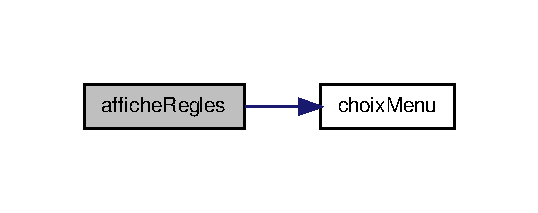
\includegraphics[width=258pt]{fonctions_affichage_8c_a6a74e3ea603ed4022ce59f1e57dbb6dd_cgraph}
\end{center}
\end{figure}




\-Voici le graphe des appelants de cette fonction \-:
\nopagebreak
\begin{figure}[H]
\begin{center}
\leavevmode
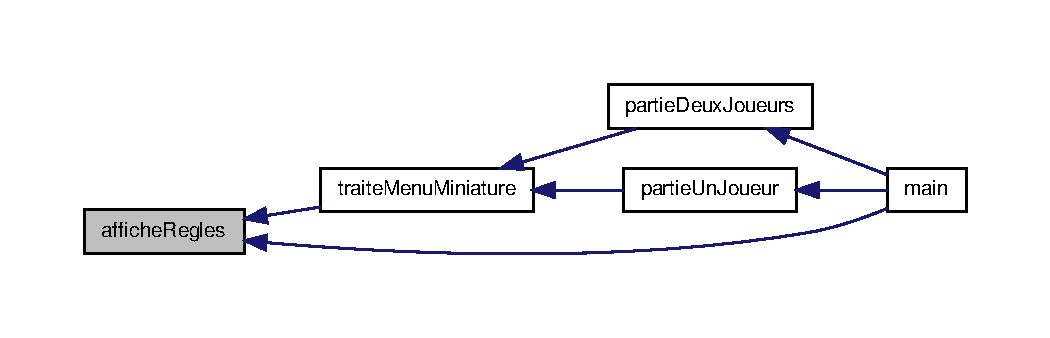
\includegraphics[width=350pt]{fonctions_affichage_8c_a6a74e3ea603ed4022ce59f1e57dbb6dd_icgraph}
\end{center}
\end{figure}


\hypertarget{fonctions_affichage_8c_aefaab0a4a9e4ccb284e6ce210fb6973b}{\index{fonctions\-Affichage.\-c@{fonctions\-Affichage.\-c}!choix\-Menu@{choix\-Menu}}
\index{choix\-Menu@{choix\-Menu}!fonctionsAffichage.c@{fonctions\-Affichage.\-c}}
\subsubsection[{choix\-Menu}]{\setlength{\rightskip}{0pt plus 5cm}short {\bf choix\-Menu} (
\begin{DoxyParamCaption}
\item[{int}]{abs\-Clic, }
\item[{int}]{ord\-Clic, }
\item[{\-S\-D\-L\-\_\-\-Rect}]{pos\-Tab\-Choix\-Menu\mbox{[}$\,$\mbox{]}}
\end{DoxyParamCaption}
)}}\label{fonctions_affichage_8c_aefaab0a4a9e4ccb284e6ce210fb6973b}


détermine si le joueur clique sur un des choix du menu 


\begin{DoxyParams}{\-Paramètres}
{\em abs\-Clic} & l'abscice du clic à traiter \\
\hline
{\em ord\-Clic} & l'ordonee du clic à traiter \\
\hline
{\em pos\-Tab\-Choix\-Menu} & \-Le tableau des position des item à traiter\\
\hline
\end{DoxyParams}
\begin{DoxyReturn}{\-Renvoie}
un nombre qui determnie un choix du menu 
\end{DoxyReturn}


\-Voici le graphe des appelants de cette fonction \-:
\nopagebreak
\begin{figure}[H]
\begin{center}
\leavevmode
\includegraphics[width=350pt]{fonctions_affichage_8c_aefaab0a4a9e4ccb284e6ce210fb6973b_icgraph}
\end{center}
\end{figure}


\hypertarget{fonctions_affichage_8c_aa0b97452ac0e386637b196b6b8105c7d}{\index{fonctions\-Affichage.\-c@{fonctions\-Affichage.\-c}!init\-Menu\-Miniature@{init\-Menu\-Miniature}}
\index{init\-Menu\-Miniature@{init\-Menu\-Miniature}!fonctionsAffichage.c@{fonctions\-Affichage.\-c}}
\subsubsection[{init\-Menu\-Miniature}]{\setlength{\rightskip}{0pt plus 5cm}void {\bf init\-Menu\-Miniature} (
\begin{DoxyParamCaption}
\item[{int}]{partie, }
\item[{\-S\-D\-L\-\_\-\-Surface $\ast$}]{tab\-Menu\-Miniature\mbox{[}$\,$\mbox{]}, }
\item[{\-T\-T\-F\-\_\-\-Font $\ast$}]{police, }
\item[{\-S\-D\-L\-\_\-\-Color}]{couleur}
\end{DoxyParamCaption}
)}}\label{fonctions_affichage_8c_aa0b97452ac0e386637b196b6b8105c7d}


initialise le menu miniature selon la partie joué 


\begin{DoxyParams}{\-Paramètres}
{\em partie} & nombre servant à savoir si on joue à 1 ou 2 joueurs \\
\hline
{\em tab\-Menu\-Miniature\mbox{[}$\,$\mbox{]}} & \-Surface contenant les item du menu \\
\hline
{\em police} & la police utilisé \\
\hline
{\em couleur} & la couleur de la police \\
\hline
\end{DoxyParams}


\-Voici le graphe des appelants de cette fonction \-:
\nopagebreak
\begin{figure}[H]
\begin{center}
\leavevmode
\includegraphics[width=350pt]{fonctions_affichage_8c_aa0b97452ac0e386637b196b6b8105c7d_icgraph}
\end{center}
\end{figure}


\hypertarget{fonctions_affichage_8c_a48262da5b852d7d777c20285f2f0b99a}{\index{fonctions\-Affichage.\-c@{fonctions\-Affichage.\-c}!traite\-Menu\-Miniature@{traite\-Menu\-Miniature}}
\index{traite\-Menu\-Miniature@{traite\-Menu\-Miniature}!fonctionsAffichage.c@{fonctions\-Affichage.\-c}}
\subsubsection[{traite\-Menu\-Miniature}]{\setlength{\rightskip}{0pt plus 5cm}short {\bf traite\-Menu\-Miniature} (
\begin{DoxyParamCaption}
\item[{int}]{abs\-Clic, }
\item[{int}]{ord\-Clic, }
\item[{\-S\-D\-L\-\_\-\-Surface $\ast$}]{ecran, }
\item[{int}]{partie}
\end{DoxyParamCaption}
)}}\label{fonctions_affichage_8c_a48262da5b852d7d777c20285f2f0b99a}


détermine si le joueur clique sur un des item du menu miniature 


\begin{DoxyParams}{\-Paramètres}
{\em abs\-Clic} & l'abscice du clic à traiter \\
\hline
{\em ord\-Clic} & l'ordonee du clic à traiter \\
\hline
{\em ecran} & la surface \-S\-D\-L où afficher les règles \\
\hline
{\em partie} & nombre servant à savoir si on joue à 1 ou 2 joueurs\\
\hline
\end{DoxyParams}
\begin{DoxyReturn}{\-Renvoie}
un nombre qui determine un choix du menu 
\end{DoxyReturn}


\-Voici le graphe d'appel pour cette fonction \-:
\nopagebreak
\begin{figure}[H]
\begin{center}
\leavevmode
\includegraphics[width=350pt]{fonctions_affichage_8c_a48262da5b852d7d777c20285f2f0b99a_cgraph}
\end{center}
\end{figure}




\-Voici le graphe des appelants de cette fonction \-:
\nopagebreak
\begin{figure}[H]
\begin{center}
\leavevmode
\includegraphics[width=350pt]{fonctions_affichage_8c_a48262da5b852d7d777c20285f2f0b99a_icgraph}
\end{center}
\end{figure}



\hypertarget{fonctions_i_a_8c}{\section{\-Référence du fichier sources/fonctions\-I\-A.c}
\label{fonctions_i_a_8c}\index{sources/fonctions\-I\-A.\-c@{sources/fonctions\-I\-A.\-c}}
}


fonctions relatives à l'inteligence artificielle  


{\ttfamily \#include \char`\"{}../headers/fonctions\-I\-A.\-h\char`\"{}}\*
\-Graphe des dépendances par inclusion de fonctions\-I\-A.\-c\-:
\nopagebreak
\begin{figure}[H]
\begin{center}
\leavevmode
\includegraphics[width=350pt]{fonctions_i_a_8c__incl}
\end{center}
\end{figure}
\subsection*{\-Fonctions}
\begin{DoxyCompactItemize}
\item 
short int \hyperlink{fonctions_i_a_8c_ae8b2b1efa750c376aeff3f38f665f76d}{evaluation\-Plateau} (\hyperlink{constantes_8h_ac19c17e9f0f0eeec3f3c11b052cfeb47}{\-Plateau} \-P)
\begin{DoxyCompactList}\small\item\em fonction evaluant si le plateau est plus ou moin favorable à l'ordi \end{DoxyCompactList}\item 
short int \hyperlink{fonctions_i_a_8c_a8d45a9c590e7a75d0b34a4f61c4e9d0b}{calcul\-Gain} (\hyperlink{constantes_8h_ac19c17e9f0f0eeec3f3c11b052cfeb47}{\-Plateau} \-P, short int couleur\-Analyse)
\begin{DoxyCompactList}\small\item\em analyse le plateau pour une couleur \end{DoxyCompactList}\item 
bool \hyperlink{fonctions_i_a_8c_a395886ef8e187f1fcf83ec3dfba2caf9}{plateau\-Vide} (\hyperlink{constantes_8h_ac19c17e9f0f0eeec3f3c11b052cfeb47}{\-Plateau} \-P, int partie\-Tableau)
\begin{DoxyCompactList}\small\item\em determine si une partie de plateau est vide ou non \end{DoxyCompactList}\item 
short int \hyperlink{fonctions_i_a_8c_a1416d179ad4f5765bbb790a77052b966}{alpha\-Beta} (\hyperlink{constantes_8h_ac19c17e9f0f0eeec3f3c11b052cfeb47}{\-Plateau} \-P, short int alpha, short int beta, short int profondeur)
\begin{DoxyCompactList}\small\item\em fonction recherchant le meilleur coup possible pour l'ordinateur en optimisant les passages dans l'arbre récursif \end{DoxyCompactList}\item 
void \hyperlink{fonctions_i_a_8c_a0e4cfe307082f42b29068d14fa592ccd}{meilleur\-Coup} (\hyperlink{constantes_8h_ac19c17e9f0f0eeec3f3c11b052cfeb47}{\-Plateau} \-P, short int couleur\-Analyse, \hyperlink{struct_coup}{\-Coup} $\ast$meilleur)
\begin{DoxyCompactList}\small\item\em détermine le meilleur coups potentiel à jouer par l'ia \end{DoxyCompactList}\end{DoxyCompactItemize}


\subsection{\-Description détaillée}
fonctions relatives à l'inteligence artificielle 

\subsection{\-Documentation des fonctions}
\hypertarget{fonctions_i_a_8c_a1416d179ad4f5765bbb790a77052b966}{\index{fonctions\-I\-A.\-c@{fonctions\-I\-A.\-c}!alpha\-Beta@{alpha\-Beta}}
\index{alpha\-Beta@{alpha\-Beta}!fonctionsIA.c@{fonctions\-I\-A.\-c}}
\subsubsection[{alpha\-Beta}]{\setlength{\rightskip}{0pt plus 5cm}short int {\bf alpha\-Beta} (
\begin{DoxyParamCaption}
\item[{{\bf \-Plateau}}]{\-P, }
\item[{short int}]{alpha, }
\item[{short int}]{beta, }
\item[{short int}]{nombre\-\_\-coups}
\end{DoxyParamCaption}
)}}\label{fonctions_i_a_8c_a1416d179ad4f5765bbb790a77052b966}


fonction recherchant le meilleur coup possible pour l'ordinateur en optimisant les passages dans l'arbre récursif 


\begin{DoxyParams}{\-Paramètres}
{\em \-P} & le plateau à évaluer \\
\hline
{\em alpha} & sert à la coupure dans les noeud max \\
\hline
{\em beta} & sert à la coupure dans les noeud min \\
\hline
{\em nombre\-\_\-coups} & pour la profondeur de l'arbre\\
\hline
\end{DoxyParams}
\begin{DoxyReturn}{\-Renvoie}
retourne le meilleur coup possible pour l'ordi 
\end{DoxyReturn}


\-Voici le graphe d'appel pour cette fonction \-:
\nopagebreak
\begin{figure}[H]
\begin{center}
\leavevmode
\includegraphics[width=350pt]{fonctions_i_a_8c_a1416d179ad4f5765bbb790a77052b966_cgraph}
\end{center}
\end{figure}




\-Voici le graphe des appelants de cette fonction \-:
\nopagebreak
\begin{figure}[H]
\begin{center}
\leavevmode
\includegraphics[width=350pt]{fonctions_i_a_8c_a1416d179ad4f5765bbb790a77052b966_icgraph}
\end{center}
\end{figure}


\hypertarget{fonctions_i_a_8c_a8d45a9c590e7a75d0b34a4f61c4e9d0b}{\index{fonctions\-I\-A.\-c@{fonctions\-I\-A.\-c}!calcul\-Gain@{calcul\-Gain}}
\index{calcul\-Gain@{calcul\-Gain}!fonctionsIA.c@{fonctions\-I\-A.\-c}}
\subsubsection[{calcul\-Gain}]{\setlength{\rightskip}{0pt plus 5cm}short int {\bf calcul\-Gain} (
\begin{DoxyParamCaption}
\item[{{\bf \-Plateau}}]{\-P, }
\item[{short int}]{couleur\-Analyse}
\end{DoxyParamCaption}
)}}\label{fonctions_i_a_8c_a8d45a9c590e7a75d0b34a4f61c4e9d0b}


analyse le plateau pour une couleur 

short int \hyperlink{fonctions_i_a_8h_a8d45a9c590e7a75d0b34a4f61c4e9d0b}{calcul\-Gain(\-Plateau P, short int couleur\-Analyse)} 
\begin{DoxyParams}{\-Paramètres}
{\em \-P} & le plateau à évaluer \\
\hline
{\em couleur\-Analyse} & represente la couleur à analyser \\
\hline
\end{DoxyParams}


\-Voici le graphe des appelants de cette fonction \-:
\nopagebreak
\begin{figure}[H]
\begin{center}
\leavevmode
\includegraphics[width=350pt]{fonctions_i_a_8c_a8d45a9c590e7a75d0b34a4f61c4e9d0b_icgraph}
\end{center}
\end{figure}


\hypertarget{fonctions_i_a_8c_ae8b2b1efa750c376aeff3f38f665f76d}{\index{fonctions\-I\-A.\-c@{fonctions\-I\-A.\-c}!evaluation\-Plateau@{evaluation\-Plateau}}
\index{evaluation\-Plateau@{evaluation\-Plateau}!fonctionsIA.c@{fonctions\-I\-A.\-c}}
\subsubsection[{evaluation\-Plateau}]{\setlength{\rightskip}{0pt plus 5cm}short int {\bf evaluation\-Plateau} (
\begin{DoxyParamCaption}
\item[{{\bf \-Plateau}}]{\-P}
\end{DoxyParamCaption}
)}}\label{fonctions_i_a_8c_ae8b2b1efa750c376aeff3f38f665f76d}


fonction evaluant si le plateau est plus ou moin favorable à l'ordi 


\begin{DoxyParams}{\-Paramètres}
{\em \-P} & le plateau à évaluer\\
\hline
\end{DoxyParams}
\begin{DoxyReturn}{\-Renvoie}
un nombre qui représente le gain 
\end{DoxyReturn}


\-Voici le graphe d'appel pour cette fonction \-:
\nopagebreak
\begin{figure}[H]
\begin{center}
\leavevmode
\includegraphics[width=278pt]{fonctions_i_a_8c_ae8b2b1efa750c376aeff3f38f665f76d_cgraph}
\end{center}
\end{figure}




\-Voici le graphe des appelants de cette fonction \-:
\nopagebreak
\begin{figure}[H]
\begin{center}
\leavevmode
\includegraphics[width=350pt]{fonctions_i_a_8c_ae8b2b1efa750c376aeff3f38f665f76d_icgraph}
\end{center}
\end{figure}


\hypertarget{fonctions_i_a_8c_a0e4cfe307082f42b29068d14fa592ccd}{\index{fonctions\-I\-A.\-c@{fonctions\-I\-A.\-c}!meilleur\-Coup@{meilleur\-Coup}}
\index{meilleur\-Coup@{meilleur\-Coup}!fonctionsIA.c@{fonctions\-I\-A.\-c}}
\subsubsection[{meilleur\-Coup}]{\setlength{\rightskip}{0pt plus 5cm}void {\bf meilleur\-Coup} (
\begin{DoxyParamCaption}
\item[{{\bf \-Plateau}}]{\-P, }
\item[{short int}]{couleur\-Analyse, }
\item[{{\bf \-Coup} $\ast$}]{meilleur}
\end{DoxyParamCaption}
)}}\label{fonctions_i_a_8c_a0e4cfe307082f42b29068d14fa592ccd}


détermine le meilleur coups potentiel à jouer par l'ia 


\begin{DoxyParams}{\-Paramètres}
{\em \-P} & le plateau à évaluer \\
\hline
{\em couleur\-Analyse} & la couleur que l'on anamyse \\
\hline
{\em meilleur} & le meileur coup possible \\
\hline
\end{DoxyParams}


\-Voici le graphe des appelants de cette fonction \-:
\nopagebreak
\begin{figure}[H]
\begin{center}
\leavevmode
\includegraphics[width=350pt]{fonctions_i_a_8c_a0e4cfe307082f42b29068d14fa592ccd_icgraph}
\end{center}
\end{figure}


\hypertarget{fonctions_i_a_8c_a395886ef8e187f1fcf83ec3dfba2caf9}{\index{fonctions\-I\-A.\-c@{fonctions\-I\-A.\-c}!plateau\-Vide@{plateau\-Vide}}
\index{plateau\-Vide@{plateau\-Vide}!fonctionsIA.c@{fonctions\-I\-A.\-c}}
\subsubsection[{plateau\-Vide}]{\setlength{\rightskip}{0pt plus 5cm}bool {\bf plateau\-Vide} (
\begin{DoxyParamCaption}
\item[{{\bf \-Plateau}}]{\-P, }
\item[{int}]{partie\-Tableau}
\end{DoxyParamCaption}
)}}\label{fonctions_i_a_8c_a395886ef8e187f1fcf83ec3dfba2caf9}


determine si une partie de plateau est vide ou non 


\begin{DoxyParams}{\-Paramètres}
{\em \-P} & le plateau à évaluer \\
\hline
{\em partie\-Tableau} & nombre representant la partie du tablea \\
\hline
\end{DoxyParams}


\-Voici le graphe d'appel pour cette fonction \-:
\nopagebreak
\begin{figure}[H]
\begin{center}
\leavevmode
\includegraphics[width=148pt]{fonctions_i_a_8c_a395886ef8e187f1fcf83ec3dfba2caf9_cgraph}
\end{center}
\end{figure}




\-Voici le graphe des appelants de cette fonction \-:
\nopagebreak
\begin{figure}[H]
\begin{center}
\leavevmode
\includegraphics[width=252pt]{fonctions_i_a_8c_a395886ef8e187f1fcf83ec3dfba2caf9_icgraph}
\end{center}
\end{figure}



\hypertarget{fonctions_plateau_8c}{\section{\-Référence du fichier sources/fonctions\-Plateau.c}
\label{fonctions_plateau_8c}\index{sources/fonctions\-Plateau.\-c@{sources/fonctions\-Plateau.\-c}}
}


fonctions relatives au plateau  


{\ttfamily \#include \char`\"{}../headers/fonctions\-Plateau.\-h\char`\"{}}\*
\-Graphe des dépendances par inclusion de fonctions\-Plateau.\-c\-:
\nopagebreak
\begin{figure}[H]
\begin{center}
\leavevmode
\includegraphics[width=350pt]{fonctions_plateau_8c__incl}
\end{center}
\end{figure}
\subsection*{\-Fonctions}
\begin{DoxyCompactItemize}
\item 
void \hyperlink{fonctions_plateau_8c_aab348cdede8cfa4104aefc0dace18e05}{\-Update\-Events} (\hyperlink{struct_input}{\-Input} $\ast$in)
\begin{DoxyCompactList}\small\item\em gestion des events selon les entrées saisis \end{DoxyCompactList}\item 
void \hyperlink{fonctions_plateau_8c_af8c205efcbda1635fd2c62ce57b535b4}{init\-Plateau} (\hyperlink{constantes_8h_ac19c17e9f0f0eeec3f3c11b052cfeb47}{\-Plateau} \-P)
\begin{DoxyCompactList}\small\item\em initialisation du plateau de cases vides \end{DoxyCompactList}\item 
void \hyperlink{fonctions_plateau_8c_ae4dba04b9a0d5d145bafae6da91baca7}{affiche\-Plateau} (\-S\-D\-L\-\_\-\-Surface $\ast$ecran, \hyperlink{constantes_8h_ac19c17e9f0f0eeec3f3c11b052cfeb47}{\-Plateau} \-P, \-S\-D\-L\-\_\-\-Surface $\ast$tab\-Emplacement\-Bille\mbox{[}$\,$\mbox{]})
\begin{DoxyCompactList}\small\item\em affichage du plateau dans la fenetre \end{DoxyCompactList}\item 
bool \hyperlink{fonctions_plateau_8c_a088863befa113f97db87b0ab58312bdf}{placer\-Bille} (\hyperlink{constantes_8h_ac19c17e9f0f0eeec3f3c11b052cfeb47}{\-Plateau} \-P, int abs\-Clic, int ord\-Clic, int nbr\-\_\-coups)
\begin{DoxyCompactList}\small\item\em placement d'une bille sur un plateau \end{DoxyCompactList}\item 
\hypertarget{fonctions_plateau_8c_ae1f612c4958da4939592b53a44e1e6f7}{int {\bfseries est\-Gagnant} (\hyperlink{constantes_8h_ac19c17e9f0f0eeec3f3c11b052cfeb47}{\-Plateau} \-P)}\label{fonctions_plateau_8c_ae1f612c4958da4939592b53a44e1e6f7}

\item 
bool \hyperlink{fonctions_plateau_8c_ac4c87ed6f29a02e05ccbc83097ff1f3c}{determiner\-Rotation} (int abs\-Clic, int ord\-Clic, \-S\-D\-L\-\_\-\-Rect tab\-Pos\-Fleche\-Rotation\mbox{[}$\,$\mbox{]}, int $\ast$\hyperlink{constantes_8h_aa65e3b592c27609a542733310b34f5d9}{sens}, int $\ast$partie\-Tableau)
\begin{DoxyCompactList}\small\item\em determiner quelle rotation il faut faire \end{DoxyCompactList}\item 
\hypertarget{fonctions_plateau_8c_a8674ce9c4c5d46b2ac20ff47d65b95f2}{void {\bfseries rotation} (\hyperlink{constantes_8h_ac19c17e9f0f0eeec3f3c11b052cfeb47}{\-Plateau} \-P, int \hyperlink{constantes_8h_aa65e3b592c27609a542733310b34f5d9}{sens}, int partie\-\_\-plateau)}\label{fonctions_plateau_8c_a8674ce9c4c5d46b2ac20ff47d65b95f2}

\end{DoxyCompactItemize}


\subsection{\-Description détaillée}
fonctions relatives au plateau 

\subsection{\-Documentation des fonctions}
\hypertarget{fonctions_plateau_8c_ae4dba04b9a0d5d145bafae6da91baca7}{\index{fonctions\-Plateau.\-c@{fonctions\-Plateau.\-c}!affiche\-Plateau@{affiche\-Plateau}}
\index{affiche\-Plateau@{affiche\-Plateau}!fonctionsPlateau.c@{fonctions\-Plateau.\-c}}
\subsubsection[{affiche\-Plateau}]{\setlength{\rightskip}{0pt plus 5cm}void {\bf affiche\-Plateau} (
\begin{DoxyParamCaption}
\item[{\-S\-D\-L\-\_\-\-Surface $\ast$}]{ecran, }
\item[{{\bf \-Plateau}}]{\-P, }
\item[{\-S\-D\-L\-\_\-\-Surface $\ast$}]{tab\-Emplacement\-Bille\mbox{[}$\,$\mbox{]}}
\end{DoxyParamCaption}
)}}\label{fonctions_plateau_8c_ae4dba04b9a0d5d145bafae6da91baca7}


affichage du plateau dans la fenetre 


\begin{DoxyParams}{\-Paramètres}
{\em ecran} & la surface \-S\-D\-L où afficher le plateau \\
\hline
{\em \-P} & le plateau à afficher \\
\hline
{\em tab\-Emplacement\-Bille\mbox{[}$\,$\mbox{]}} & tableau contenant les coordonnées de chaque bille \\
\hline
\end{DoxyParams}


\-Voici le graphe des appelants de cette fonction \-:
\nopagebreak
\begin{figure}[H]
\begin{center}
\leavevmode
\includegraphics[width=350pt]{fonctions_plateau_8c_ae4dba04b9a0d5d145bafae6da91baca7_icgraph}
\end{center}
\end{figure}


\hypertarget{fonctions_plateau_8c_ac4c87ed6f29a02e05ccbc83097ff1f3c}{\index{fonctions\-Plateau.\-c@{fonctions\-Plateau.\-c}!determiner\-Rotation@{determiner\-Rotation}}
\index{determiner\-Rotation@{determiner\-Rotation}!fonctionsPlateau.c@{fonctions\-Plateau.\-c}}
\subsubsection[{determiner\-Rotation}]{\setlength{\rightskip}{0pt plus 5cm}bool {\bf determiner\-Rotation} (
\begin{DoxyParamCaption}
\item[{int}]{abs\-Clic, }
\item[{int}]{ord\-Clic, }
\item[{\-S\-D\-L\-\_\-\-Rect}]{tab\-Pos\-Fleche\-Rotation\mbox{[}$\,$\mbox{]}, }
\item[{int $\ast$}]{sens, }
\item[{int $\ast$}]{partie\-Tableau}
\end{DoxyParamCaption}
)}}\label{fonctions_plateau_8c_ac4c87ed6f29a02e05ccbc83097ff1f3c}


determiner quelle rotation il faut faire 


\begin{DoxyParams}{\-Paramètres}
{\em abs\-Clic} & abscice de la souris \\
\hline
{\em ord\-Clic} & ordonne de la souris \\
\hline
{\em tab\-Pos\-Fleche\-Rotation\mbox{[}$\,$\mbox{]}} & pour savoir la position des flèches a l'écran \\
\hline
{\em sens} & le sens de rotation a effectuer \\
\hline
{\em partie\-Tableau} & sur quelle partie du plateau on effectue la rotation\\
\hline
\end{DoxyParams}
\begin{DoxyReturn}{\-Renvoie}
vrais si on doit faire une rotation çàd si on a cliquer sur une flêche 
\end{DoxyReturn}


\-Voici le graphe des appelants de cette fonction \-:
\nopagebreak
\begin{figure}[H]
\begin{center}
\leavevmode
\includegraphics[width=350pt]{fonctions_plateau_8c_ac4c87ed6f29a02e05ccbc83097ff1f3c_icgraph}
\end{center}
\end{figure}


\hypertarget{fonctions_plateau_8c_af8c205efcbda1635fd2c62ce57b535b4}{\index{fonctions\-Plateau.\-c@{fonctions\-Plateau.\-c}!init\-Plateau@{init\-Plateau}}
\index{init\-Plateau@{init\-Plateau}!fonctionsPlateau.c@{fonctions\-Plateau.\-c}}
\subsubsection[{init\-Plateau}]{\setlength{\rightskip}{0pt plus 5cm}void {\bf init\-Plateau} (
\begin{DoxyParamCaption}
\item[{{\bf \-Plateau}}]{\-P}
\end{DoxyParamCaption}
)}}\label{fonctions_plateau_8c_af8c205efcbda1635fd2c62ce57b535b4}


initialisation du plateau de cases vides 


\begin{DoxyParams}{\-Paramètres}
{\em \-P} & le plateau à initialiser \\
\hline
\end{DoxyParams}


\-Voici le graphe des appelants de cette fonction \-:
\nopagebreak
\begin{figure}[H]
\begin{center}
\leavevmode
\includegraphics[width=350pt]{fonctions_plateau_8c_af8c205efcbda1635fd2c62ce57b535b4_icgraph}
\end{center}
\end{figure}


\hypertarget{fonctions_plateau_8c_a088863befa113f97db87b0ab58312bdf}{\index{fonctions\-Plateau.\-c@{fonctions\-Plateau.\-c}!placer\-Bille@{placer\-Bille}}
\index{placer\-Bille@{placer\-Bille}!fonctionsPlateau.c@{fonctions\-Plateau.\-c}}
\subsubsection[{placer\-Bille}]{\setlength{\rightskip}{0pt plus 5cm}bool {\bf placer\-Bille} (
\begin{DoxyParamCaption}
\item[{{\bf \-Plateau}}]{\-P, }
\item[{int}]{abs\-Clic, }
\item[{int}]{ord\-Clic, }
\item[{int}]{nombre\-\_\-coups}
\end{DoxyParamCaption}
)}}\label{fonctions_plateau_8c_a088863befa113f97db87b0ab58312bdf}


placement d'une bille sur un plateau 


\begin{DoxyParams}{\-Paramètres}
{\em \-P} & le plateau uitilisé \\
\hline
{\em abs\-Clic} & abscice de la souris \\
\hline
{\em ord\-Clic} & ordonne de la souris \\
\hline
{\em nombre\-\_\-coups} & nombre qui sert a determiner si on place une bille noire ou blanche\\
\hline
\end{DoxyParams}
\begin{DoxyReturn}{\-Renvoie}
vrais si une bille a été placée 
\end{DoxyReturn}


\-Voici le graphe des appelants de cette fonction \-:
\nopagebreak
\begin{figure}[H]
\begin{center}
\leavevmode
\includegraphics[width=350pt]{fonctions_plateau_8c_a088863befa113f97db87b0ab58312bdf_icgraph}
\end{center}
\end{figure}


\hypertarget{fonctions_plateau_8c_aab348cdede8cfa4104aefc0dace18e05}{\index{fonctions\-Plateau.\-c@{fonctions\-Plateau.\-c}!\-Update\-Events@{\-Update\-Events}}
\index{\-Update\-Events@{\-Update\-Events}!fonctionsPlateau.c@{fonctions\-Plateau.\-c}}
\subsubsection[{\-Update\-Events}]{\setlength{\rightskip}{0pt plus 5cm}void {\bf \-Update\-Events} (
\begin{DoxyParamCaption}
\item[{{\bf \-Input} $\ast$}]{in}
\end{DoxyParamCaption}
)}}\label{fonctions_plateau_8c_aab348cdede8cfa4104aefc0dace18e05}


gestion des events selon les entrées saisis 


\begin{DoxyParams}{\-Paramètres}
{\em in} & les entrées saisis \\
\hline
\end{DoxyParams}


\-Voici le graphe des appelants de cette fonction \-:
\nopagebreak
\begin{figure}[H]
\begin{center}
\leavevmode
\includegraphics[width=350pt]{fonctions_plateau_8c_aab348cdede8cfa4104aefc0dace18e05_icgraph}
\end{center}
\end{figure}



\hypertarget{main_8c}{\section{\-Référence du fichier sources/main.c}
\label{main_8c}\index{sources/main.\-c@{sources/main.\-c}}
}


fonction principale du jeu  


{\ttfamily \#include \char`\"{}../headers/fonctions\-Affichage.\-h\char`\"{}}\*
\-Graphe des dépendances par inclusion de main.\-c\-:
\nopagebreak
\begin{figure}[H]
\begin{center}
\leavevmode
\includegraphics[width=350pt]{main_8c__incl}
\end{center}
\end{figure}
\subsection*{\-Fonctions}
\begin{DoxyCompactItemize}
\item 
int \hyperlink{main_8c_a3c04138a5bfe5d72780bb7e82a18e627}{main} (int argc, char $\ast$$\ast$argv)
\begin{DoxyCompactList}\small\item\em premier fonction utilisée au lancement du programme \end{DoxyCompactList}\end{DoxyCompactItemize}


\subsection{\-Description détaillée}
fonction principale du jeu 

\subsection{\-Documentation des fonctions}
\hypertarget{main_8c_a3c04138a5bfe5d72780bb7e82a18e627}{\index{main.\-c@{main.\-c}!main@{main}}
\index{main@{main}!main.c@{main.\-c}}
\subsubsection[{main}]{\setlength{\rightskip}{0pt plus 5cm}int {\bf main} (
\begin{DoxyParamCaption}
\item[{int}]{argc, }
\item[{char $\ast$$\ast$}]{argv}
\end{DoxyParamCaption}
)}}\label{main_8c_a3c04138a5bfe5d72780bb7e82a18e627}


premier fonction utilisée au lancement du programme 


\begin{DoxyParams}{\-Paramètres}
{\em argc} & nombre de chaine contenue dans argv \\
\hline
{\em argv} & argument pour lancer le programme\\
\hline
\end{DoxyParams}
\begin{DoxyReturn}{\-Renvoie}
0 si le programme c'est bien exécutée 
\end{DoxyReturn}


\-Voici le graphe d'appel pour cette fonction \-:
\nopagebreak
\begin{figure}[H]
\begin{center}
\leavevmode
\includegraphics[width=350pt]{main_8c_a3c04138a5bfe5d72780bb7e82a18e627_cgraph}
\end{center}
\end{figure}



\hypertarget{partie_deux_joueurs_8c}{\section{\-Référence du fichier sources/partie\-Deux\-Joueurs.c}
\label{partie_deux_joueurs_8c}\index{sources/partie\-Deux\-Joueurs.\-c@{sources/partie\-Deux\-Joueurs.\-c}}
}


fonctions gérant le mode 2 joueurs  


{\ttfamily \#include \char`\"{}../headers/partie\-Deux\-Joueurs.\-h\char`\"{}}\*
{\ttfamily \#include \char`\"{}../headers/fonctions\-Plateau.\-h\char`\"{}}\*
\-Graphe des dépendances par inclusion de partie\-Deux\-Joueurs.\-c\-:
\nopagebreak
\begin{figure}[H]
\begin{center}
\leavevmode
\includegraphics[width=350pt]{partie_deux_joueurs_8c__incl}
\end{center}
\end{figure}
\subsection*{\-Fonctions}
\begin{DoxyCompactItemize}
\item 
int \hyperlink{partie_deux_joueurs_8c_a374909eadd0b6ee203667f93f32342ec}{partie\-Deux\-Joueurs} (\-S\-D\-L\-\_\-\-Surface $\ast$ecran)
\begin{DoxyCompactList}\small\item\em permet de jouer contre un joueur \end{DoxyCompactList}\end{DoxyCompactItemize}


\subsection{\-Description détaillée}
fonctions gérant le mode 2 joueurs 

\subsection{\-Documentation des fonctions}
\hypertarget{partie_deux_joueurs_8c_a374909eadd0b6ee203667f93f32342ec}{\index{partie\-Deux\-Joueurs.\-c@{partie\-Deux\-Joueurs.\-c}!partie\-Deux\-Joueurs@{partie\-Deux\-Joueurs}}
\index{partie\-Deux\-Joueurs@{partie\-Deux\-Joueurs}!partieDeuxJoueurs.c@{partie\-Deux\-Joueurs.\-c}}
\subsubsection[{partie\-Deux\-Joueurs}]{\setlength{\rightskip}{0pt plus 5cm}int {\bf partie\-Deux\-Joueurs} (
\begin{DoxyParamCaption}
\item[{\-S\-D\-L\-\_\-\-Surface $\ast$}]{ecran}
\end{DoxyParamCaption}
)}}\label{partie_deux_joueurs_8c_a374909eadd0b6ee203667f93f32342ec}


permet de jouer contre un joueur 


\begin{DoxyParams}{\-Paramètres}
{\em ecran} & affiche le jeu\\
\hline
\end{DoxyParams}
\begin{DoxyReturn}{\-Renvoie}
un nombre qui determine les actions de fin de jeu 
\end{DoxyReturn}


\-Voici le graphe d'appel pour cette fonction \-:
\nopagebreak
\begin{figure}[H]
\begin{center}
\leavevmode
\includegraphics[width=350pt]{partie_deux_joueurs_8c_a374909eadd0b6ee203667f93f32342ec_cgraph}
\end{center}
\end{figure}




\-Voici le graphe des appelants de cette fonction \-:
\nopagebreak
\begin{figure}[H]
\begin{center}
\leavevmode
\includegraphics[width=252pt]{partie_deux_joueurs_8c_a374909eadd0b6ee203667f93f32342ec_icgraph}
\end{center}
\end{figure}



\hypertarget{partie_un_joueur_8c}{\section{\-Référence du fichier sources/partie\-Un\-Joueur.c}
\label{partie_un_joueur_8c}\index{sources/partie\-Un\-Joueur.\-c@{sources/partie\-Un\-Joueur.\-c}}
}


fonctions gérant le mode 1 joueur  


{\ttfamily \#include \char`\"{}../headers/partie\-Un\-Joueur.\-h\char`\"{}}\*
{\ttfamily \#include \char`\"{}../headers/fonctions\-Plateau.\-h\char`\"{}}\*
\-Graphe des dépendances par inclusion de partie\-Un\-Joueur.\-c\-:
\nopagebreak
\begin{figure}[H]
\begin{center}
\leavevmode
\includegraphics[width=350pt]{partie_un_joueur_8c__incl}
\end{center}
\end{figure}
\subsection*{\-Fonctions}
\begin{DoxyCompactItemize}
\item 
int \hyperlink{partie_un_joueur_8c_a4abb180c273289e30fd8dd09696265f8}{partie\-Un\-Joueur} (\-S\-D\-L\-\_\-\-Surface $\ast$ecran)
\begin{DoxyCompactList}\small\item\em permet de jouer contre l'ordinateur \end{DoxyCompactList}\end{DoxyCompactItemize}


\subsection{\-Description détaillée}
fonctions gérant le mode 1 joueur 

\subsection{\-Documentation des fonctions}
\hypertarget{partie_un_joueur_8c_a4abb180c273289e30fd8dd09696265f8}{\index{partie\-Un\-Joueur.\-c@{partie\-Un\-Joueur.\-c}!partie\-Un\-Joueur@{partie\-Un\-Joueur}}
\index{partie\-Un\-Joueur@{partie\-Un\-Joueur}!partieUnJoueur.c@{partie\-Un\-Joueur.\-c}}
\subsubsection[{partie\-Un\-Joueur}]{\setlength{\rightskip}{0pt plus 5cm}int {\bf partie\-Un\-Joueur} (
\begin{DoxyParamCaption}
\item[{\-S\-D\-L\-\_\-\-Surface $\ast$}]{ecran}
\end{DoxyParamCaption}
)}}\label{partie_un_joueur_8c_a4abb180c273289e30fd8dd09696265f8}


permet de jouer contre l'ordinateur 


\begin{DoxyParams}{\-Paramètres}
{\em ecran} & affiche le jeu\\
\hline
\end{DoxyParams}
\begin{DoxyReturn}{\-Renvoie}
un nombre qui determine les actions de fin de jeu 
\end{DoxyReturn}


\-Voici le graphe d'appel pour cette fonction \-:
\nopagebreak
\begin{figure}[H]
\begin{center}
\leavevmode
\includegraphics[width=350pt]{partie_un_joueur_8c_a4abb180c273289e30fd8dd09696265f8_cgraph}
\end{center}
\end{figure}




\-Voici le graphe des appelants de cette fonction \-:
\nopagebreak
\begin{figure}[H]
\begin{center}
\leavevmode
\includegraphics[width=238pt]{partie_un_joueur_8c_a4abb180c273289e30fd8dd09696265f8_icgraph}
\end{center}
\end{figure}



\printindex
\end{document}
